%% ==============================================================================
%% CO3133: Deep Learning and Its Applications — Assignment 01 (Semester 261)
%% Comprehensive Final Technical Report: Integrating Milestone 1 (M1) and Milestone 2 (M2)
%% Official Submission Document: Goat_A1_Report.pdf
%% Author: Hoàng Trọng Huy Minh (Student ID: 2452743) — Sole Contributor (100%)
%% Faculty of Computer Science & Engineering, HCMUT — VNU-HCM
%% ==============================================================================
\documentclass[11pt, a4paper]{article}

% ---- Essential Academic Packages ----------------------------------------------
\usepackage{geometry}
\geometry{top=2.2cm, bottom=2.2cm, left=2.2cm, right=2.2cm}
\usepackage{graphicx}
\usepackage{subcaption}
\usepackage{booktabs}
\usepackage{amsmath, amssymb, amsfonts}
\usepackage{hyperref}
\usepackage{xcolor}
\usepackage{listings}
\usepackage{enumitem}
\usepackage{float}
\usepackage{caption}
\usepackage{array}
\usepackage{multirow}
\usepackage{setspace}
\usepackage{fancyhdr}
\usepackage{tabularx}
\usepackage{adjustbox}

% ---- Color Palette -----------------------------------------------------------
\definecolor{navyblue}{RGB}{11, 42, 74}
\definecolor{deepcyan}{RGB}{22, 166, 182}
\definecolor{darkslate}{RGB}{23, 50, 77}
\definecolor{codebg}{RGB}{248, 250, 252}
\definecolor{codeframe}{RGB}{226, 232, 240}
\definecolor{darkgreen}{RGB}{5, 150, 105}

\hypersetup{
    colorlinks=true,
    linkcolor=navyblue,
    urlcolor=deepcyan,
    citecolor=navyblue,
    pdfauthor={Hoang Trong Huy Minh (2452743)},
    pdftitle={CO3133 Assignment 01 Cumulative Final Report (M1 + M2) - Group Goat}
}

% ---- Tabularx Column Types ----------------------------------------------------
\newcolumntype{Y}{>{\centering\arraybackslash}X}
\newcolumntype{L}{>{\raggedright\arraybackslash}X}

% ---- Code Listing Settings ---------------------------------------------------
\lstset{
  backgroundcolor=\color{codebg},
  frame=single,
  rulecolor=\color{codeframe},
  basicstyle=\ttfamily\footnotesize,
  keywordstyle=\color{navyblue}\bfseries,
  commentstyle=\color{gray}\itshape,
  stringstyle=\color{darkgreen},
  breaklines=true,
  numbers=left,
  numberstyle=\tiny\color{gray},
  stepnumber=1,
  tabsize=2,
  language=Python,
  showstringspaces=false
}

% ---- Running Headers & Footers -----------------------------------------------
\pagestyle{fancy}
\fancyhf{}
\rhead{\footnotesize\textcolor{navyblue}{\textbf{CO3133: Deep Learning} --- Assignment 1 (M1 + M2 Final)}}
\lhead{\footnotesize\textcolor{navyblue}{Group Goat --- HCMUT}}
\rfoot{\footnotesize Page \thepage}
\lfoot{\footnotesize\textcolor{gray}{Author: Hoàng Trọng Huy Minh (2452743)}}
\renewcommand{\headrulewidth}{0.5pt}
\renewcommand{\footrulewidth}{0.3pt}

% ---- Document Content ---------------------------------------------------------
\begin{document}

% ---- Title Block with Institutional Emblem -----------------------------------
\begin{center}
  
\includegraphics[height=2.7cm]{hcmut_logo.png}\\[0.6em]
  {\Large\scshape Ho Chi Minh City University of Technology (HCMUT) --- VNU-HCM}\\[0.3em]
  {\large\scshape Faculty of Computer Science and Engineering}\\[0.5em]
  \rule{\textwidth}{1.2pt}\\[0.7em]
  {\LARGE\bfseries CO3133: Deep Learning and Its Applications}\\[0.3em]
  {\Large\bfseries Assignment 01: Foundations of Deep Learning Pipelines and Architectures}\\[0.3em]
  {\large\textbf{Comprehensive Cumulative Technical Report: Integrating Milestone 1 (M1) and Milestone 2 (M2)}}\\[0.6em]
  \rule{\textwidth}{1.2pt}\\[0.8em]
\end{center}

\begin{table}[H]
  \centering
  \small
  \begin{tabularx}{\textwidth}{@{}p{3.8cm} X@{}}
    \textbf{Course Code / Term:} & CO3133 --- Semester 261 (Academic Year 2026--2027) \\
    \textbf{Instructor:}         & Assoc. Prof. Lê Thành Sách \\
    \textbf{Group Identifier:}   & Group Goat \\
    \textbf{Author \& Lead:}     & \textbf{Hoàng Trọng Huy Minh} (Student ID: \textbf{2452743}) --- \textbf{100\% Contribution (Sole Contributor)} \\
    \textbf{Other Group Members:}& Võ Lê Thành Triệu (2453297, 0\%), Nguyễn Huỳnh Nam Quốc (2453089, 0\%) \\
    \textbf{Project Repository:} & \url{https://github.com/volethanhtrieu/DL_Assignment-01} \\
    \textbf{Interactive Webpage:}& \url{https://volethanhtrieu.github.io/Deep-Learning-project-main-page/assignment-01/} \\
    \textbf{Report Scope:}       & Full Cumulative Submission rigorously covering \textbf{Milestone 1} and \textbf{Milestone 2} \\
    \textbf{Submission Date:}    & October 2026 (Final Official Deliverable) \\
  \end{tabularx}
\end{table}

\begin{abstract}
\noindent
This document constitutes the comprehensive, cumulative technical report for **Assignment 01** of **CO3133: Deep Learning and Its Applications** at Ho Chi Minh City University of Technology (HCMUT). Rather than isolating late-stage models, this report provides a fully unified scientific account across the two developmental phases mandated by the Course Project Handbook:
\begin{enumerate}[noitemsep]
  \item \textbf{Milestone 1 (Foundational Pipeline and Flat Baselines)}: Rigorous Exploratory Data Analysis (EDA) of Fashion-MNIST ($70{,}000$ instances, 10 classes) spanning 5 analytical figures; formulation of a strictly leak-free, stratified DataLoader ($50{,}000$ train / $10{,}000$ val / $10{,}000$ test, Seed 42); implementation of a standardized training engine with AdamW, Cosine Annealing, and Early Stopping on validation Macro-F1; and exhaustive benchmarking of foundational permutation-invariant models: a \textbf{Linear Softmax Classifier} ($7{,}850$ params) and a 2-hidden-layer \textbf{Multilayer Perceptron (MLP)} ($235{,}146$ params).
  \item \textbf{Milestone 2 (Advanced Inductive Bias and Sequence Scaling)}: Scaling beyond flat feature vectors by designing and training from scratch three advanced structural paradigms: a \textbf{Custom 3-Stage Convolutional Neural Network (CNN)} ($94{,}186$ params) with spatial locality priors; a \textbf{Bidirectional Row-Sequence Recurrent Network (Bi-LSTM)} ($149{,}002$ params) modeling vertical garment silhouettes; and a patch-based \textbf{Vision Transformer (ViT)} ($105{,}546$ params) operating via multi-head self-attention.
\end{enumerate}
All five architectures were trained under identical hardware (NVIDIA RTX 3060) and optimization budgets, and evaluated against the isolated $10{,}000$-sample test set. Our empirical findings demonstrate that: (i) the custom CNN achieves the highest classification accuracy ($90.26\%$) and Macro-F1 ($90.26\%$) with only $94{,}186$ parameters, outperforming the $235\text{k}$-parameter MLP by $+1.40\%$ while slashing parameter count by $60\%$; (ii) the Bi-LSTM ranks second ($89.65\%$ Acc, $89.61\%$ Macro-F1), proving that sequential row scanning effectively tracks apparel contours; (iii) the Vision Transformer trained from scratch achieves $88.07\%$ accuracy, demonstrating viable global attention but limited by lack of spatial inductive bias on moderate data; and (iv) the MLP ($88.86\%$) decisively outperforms the Linear baseline ($84.49\%$), proving the mathematical necessity of non-linear decision boundaries. Full training curves, $10 \times 10$ confusion matrices, inference latencies, per-class F1 progression, qualitative prediction error taxonomies, ablations, and a 9-field academic integrity disclosure are presented.
\end{abstract}

\tableofcontents
\newpage

% ==============================================================================
\part{Problem Formulation, Data Engineering, and M1 Foundations}
\label{part:data_m1}
% ==============================================================================

\section{Problem Formulation and Integrated Milestone Framework}
\label{sec:problem_formulation}

\subsection{Real-World Motivation}
Automated fashion apparel recognition is a core technological driver of modern visual search, e-commerce cataloging, inventory auditing, and robotic supply chains. In contrast to synthetic optical character recognition (e.g., MNIST digit classification), clothing classification presents severe real-world computer vision challenges:
\begin{itemize}[noitemsep]
  \item \textbf{High Intra-Class Variation}: Garments of the same category vary drastically in fabric draping, sleeve extensions, buttoning styles, and neckline geometries.
  \item \textbf{Severe Inter-Class Visual Overlap}: Multiple apparel categories share nearly identical coarse spatial silhouettes (e.g., \textit{Shirt} vs. \textit{T-shirt/top}, \textit{Pullover} vs. \textit{Coat}).
  \item \textbf{Low-Resolution Ambiguity}: In $28 \times 28$ grayscale images, discriminative micro-textures (collar seams, button plackets, weave patterns) are compressed into single-pixel variations, demanding architectures with strong inductive biases.
\end{itemize}

\subsection{Mathematical Formulation}
Let $\mathcal{X} \subset \mathbb{R}^{H \times W} = \mathbb{R}^{28 \times 28}$ denote the input space of normalized grayscale fashion images, and let $\mathcal{Y} = \{0, 1, \ldots, 9\}$ denote the discrete label space representing 10 mutually exclusive clothing categories. The dataset comprises $N$ independent and identically distributed pairs:
\begin{equation}
  \mathcal{D} = \{(\mathbf{x}_i, y_i)\}_{i=1}^N, \quad \mathbf{x}_i \in \mathbb{R}^{28 \times 28}, \; y_i \in \mathcal{Y}.
\end{equation}
The core objective is to parameterize and optimize a deep neural network hypothesis $f_\theta: \mathcal{X} \to \mathbb{R}^{10}$ producing unnormalized class logits $\mathbf{z} = f_\theta(\mathbf{x})$ such that the empirical risk under the multi-class Cross-Entropy loss is minimized:
\begin{equation}
  \min_{\theta} \mathcal{R}_{\text{emp}}(\theta) = \frac{1}{|\mathcal{D}_{\text{train}}|} \sum_{(\mathbf{x}_i, y_i) \in \mathcal{D}_{\text{train}}} \mathcal{L}_{\text{CE}}(f_\theta(\mathbf{x}_i), y_i) + \lambda \Omega(\theta),
\end{equation}
where $\Omega(\theta) = \frac{1}{2}\|\theta\|_2^2$ represents decoupled $L_2$ weight regularization, and the posterior probability for class $k \in \mathcal{Y}$ is recovered via the softmax function:
\begin{equation}
  P(y = k \mid \mathbf{x}) = \frac{\exp(z_k)}{\sum_{j=0}^9 \exp(z_j)}.
\end{equation}

\subsection{Integrated Milestone Framework (M1 Foundations to M2 Advancements)}
Table~\ref{tab:milestone_structure} outlines the two-phase developmental architecture mandated in the Course Project Handbook (Section~7.4). Rather than treating M1 and M2 as disparate milestones, this report demonstrates their deep structural continuity: Milestone 1 established the empirical baseline, data integrity protocols, and training engine upon which Milestone 2 systematically benchmarked advanced inductive biases.

\begin{table}[H]
  \centering
  \caption{Course Project Assignment 1 Integrated Milestone Breakdown (Handbook Section 7.4).}
  \label{tab:milestone_structure}
  \small
  \begin{tabularx}{\textwidth}{@{}p{3.2cm} c p{4.2cm} X@{}}
    \toprule
    \textbf{Project Phase} & \textbf{Timeline} & \textbf{Core Methodological Focus} & \textbf{Concrete Deliverables} \\
    \midrule
    \textbf{Milestone 1 (M1)} & September 2026 & Problem formulation, 5-figure EDA, stratified leak-free DataLoader, training engine, early stopping, Linear and MLP baselines. & Initial draft report, 5 EDA figures, training history CSV/JSON, Linear and MLP checkpoints, baseline curves and confusion matrices. \\
    \textbf{Milestone 2 (M2)} & October 2026 & Scaling to 3 advanced families (CNN, Bi-LSTM, ViT), 5-model master benchmark, error taxonomy, ablations, webpage, presentation. & Cumulative technical report (\texttt{Goat\_A1\_Report.pdf}), 5 saved checkpoints, interactive GitHub Pages site, presentation deck, video outline. \\
    \bottomrule
  \end{tabularx}
\end{table}

% ------------------------------------------------------------------------------
\section{Fashion-MNIST Exploratory Data Analysis (M1 Core Deliverable)}
\label{sec:eda}

\subsection{Dataset Provenance and Benchmark Properties}
Fashion-MNIST \cite{xiao2017fashionmnist} was introduced by Zalando Research as a drop-in replacement for MNIST to challenge deep learning models with realistic visual complexity. Table~\ref{tab:dataset_specs} details its key technical specifications.

\begin{table}[H]
  \centering
  \caption{Fashion-MNIST technical specifications and benchmark properties.}
  \label{tab:dataset_specs}
  \small
  \begin{tabularx}{\textwidth}{@{}p{3.8cm} p{4.2cm} X@{}}
    \toprule
    \textbf{Specification Property} & \textbf{Value / Configuration} & \textbf{Design Justification / Impact} \\
    \midrule
    Total Image Count & 70,000 instances & Statistical power for multi-model benchmarking \\
    Spatial Resolution & $28 \times 28$ pixels (Grayscale) & Controlled input complexity ($784$ features) \\
    Number of Classes & 10 mutually exclusive categories & Comprehensive multi-class evaluation across apparel forms \\
    Benchmark Split & 60,000 Train / 10,000 Test & Standard benchmark evaluation protocol \\
    Pixel Dynamic Range & $[0, 255]$ (uint8) $\to [0, 1]$ Float & Normalized input for numerical gradient stability \\
    Empirical Normalization & $\mu = 0.2860, \; \sigma = 0.3530$ & Zero-centering across training benchmark \\
    Storage Footprint & $\sim 30$ MB compressed & Enables low-latency in-memory batch transfer \\
    License & MIT License & Open academic research reproducibility \\
    \bottomrule
  \end{tabularx}
\end{table}

\subsection{Class Distribution and Imbalance Verification}
Data imbalance can severely distort classification performance by rewarding trivial majority-class predictions while suppressing minority Macro-F1 scores. Figure~\ref{fig:class_dist} confirms that Fashion-MNIST is \textbf{perfectly balanced}:
\begin{itemize}[noitemsep]
  \item Exactly $6{,}000$ images per class in the official $60{,}000$ training collection.
  \item Exactly $1{,}000$ images per class in the official $10{,}000$ test partition.
  \item The imbalance ratio is strictly $1.000:1$ across all 10 categories, confirming that class-weighted loss rebalancing or synthetic sampling is unnecessary.
\end{itemize}

\begin{figure}[H]
  \centering
  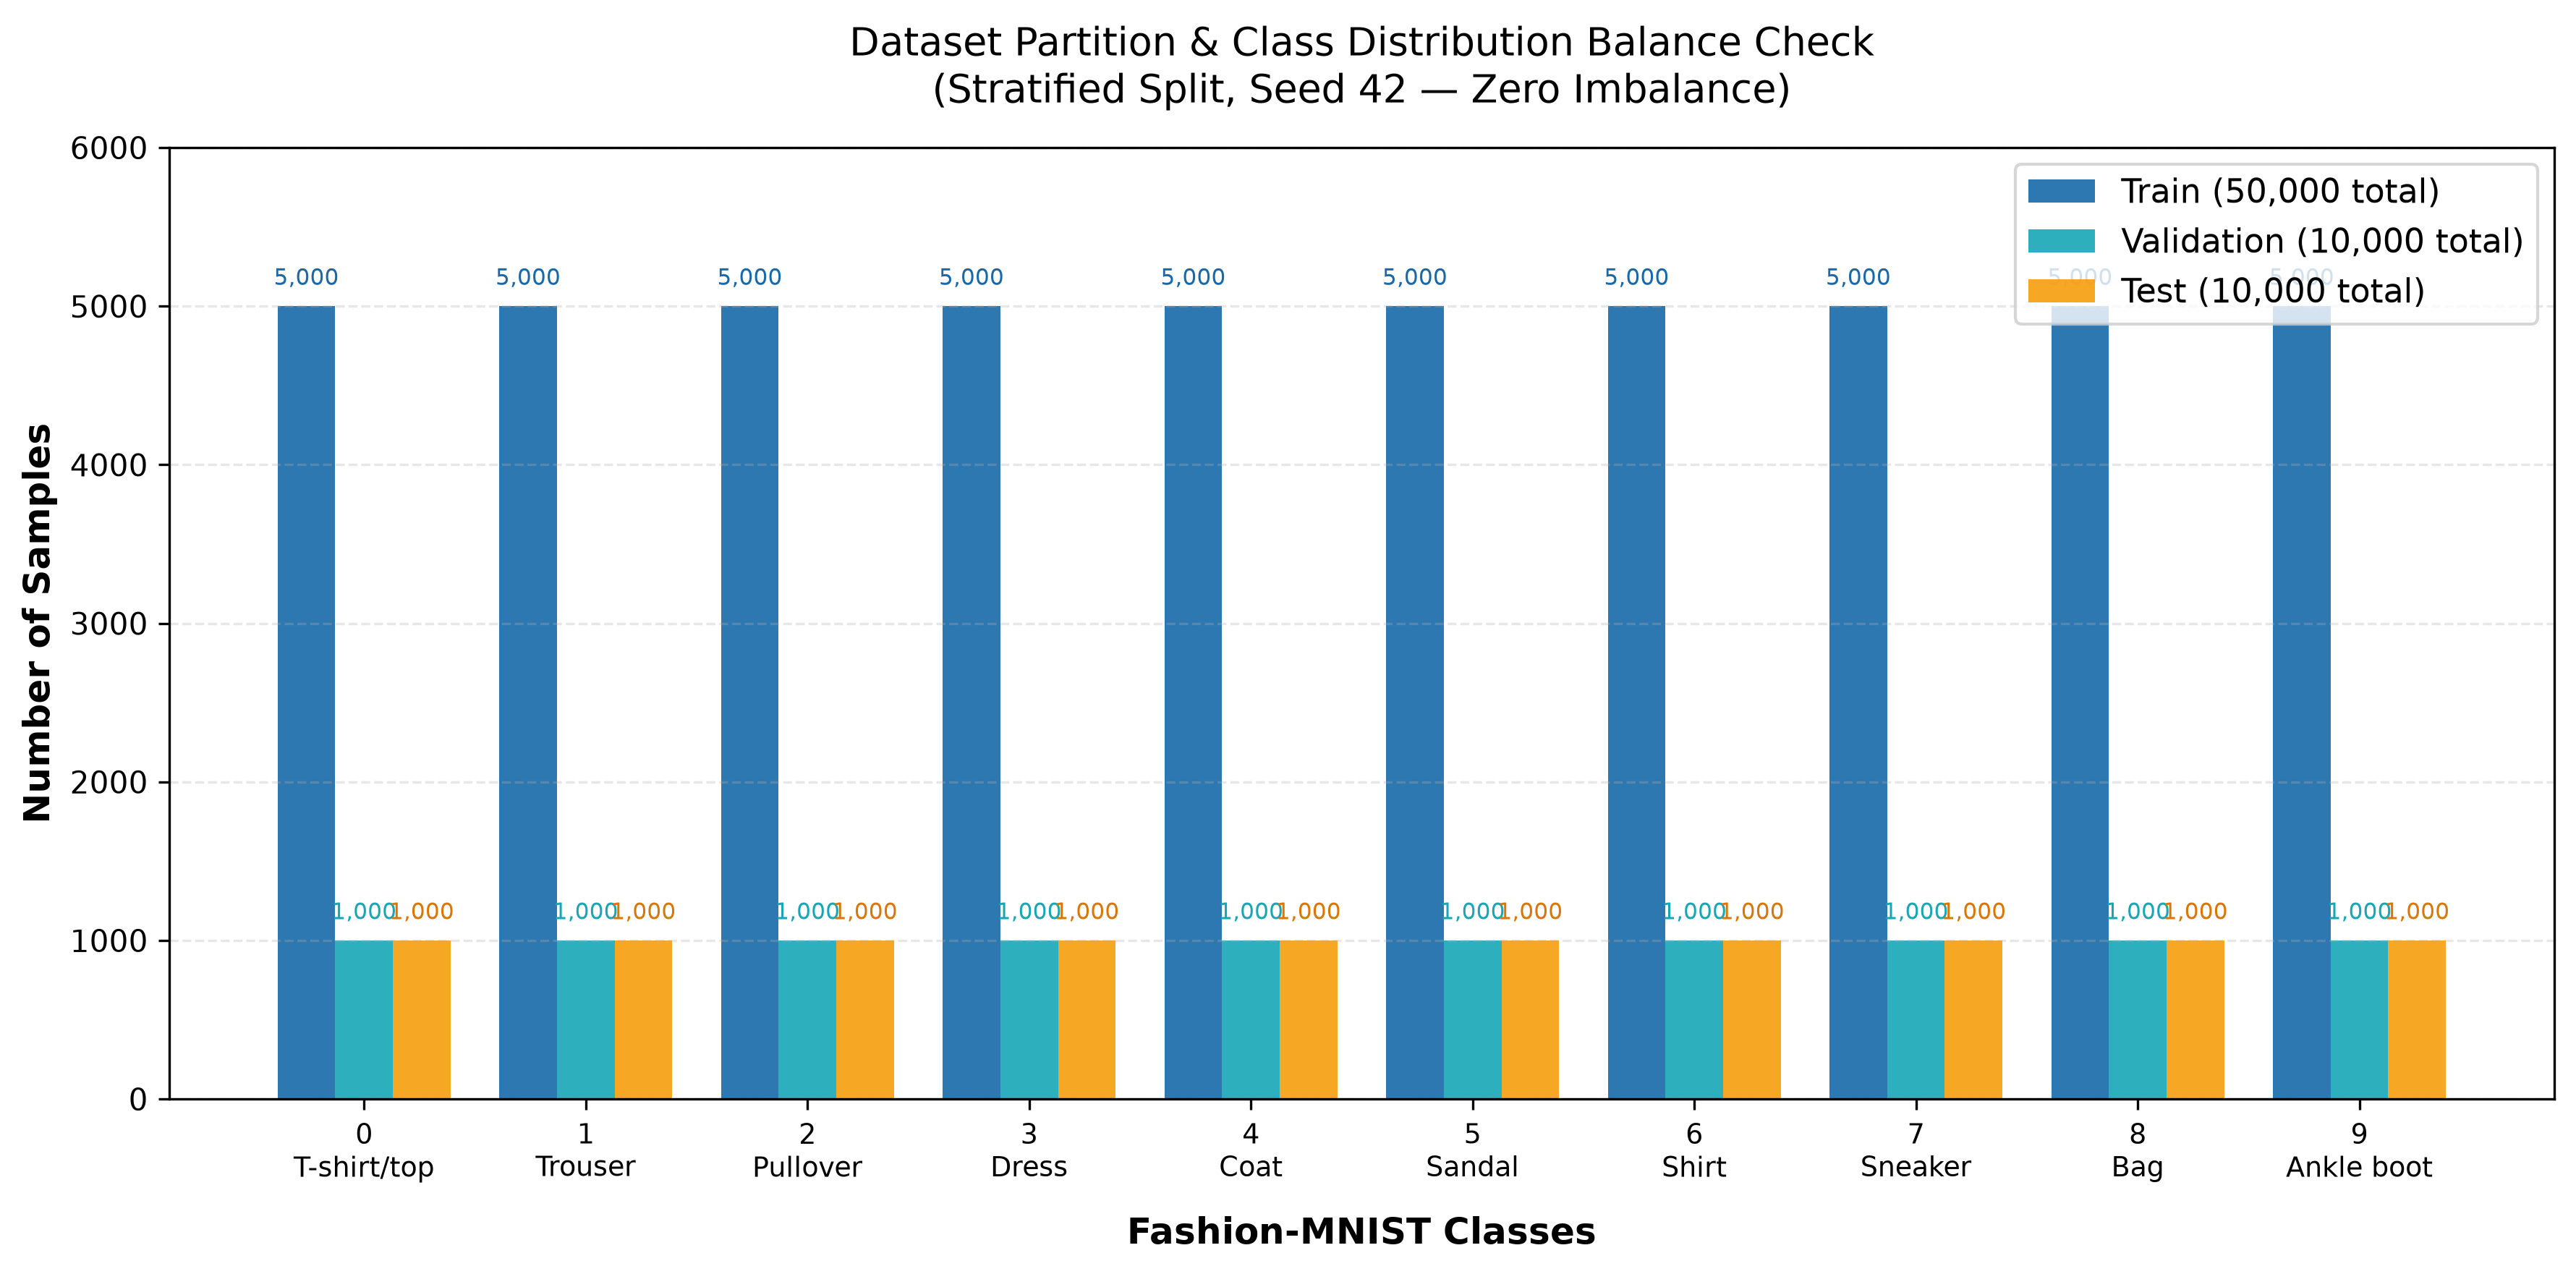
\includegraphics[width=0.68\textwidth]{eda_figures/fig2_class_distribution.png}
  \caption{Class distribution across data splits. Each category contains exactly 5,000 train, 1,000 validation, and 1,000 test instances, proving zero class imbalance.}
  \label{fig:class_dist}
\end{figure}

\subsection{Visual Inspection of Representative Samples}
Figure~\ref{fig:rep_samples} illustrates randomly sampled instances from each category ($10 \times 5$ grid). Visual inspection categorizes the apparel into distinct morphological clusters:
\begin{enumerate}[noitemsep]
  \item \textbf{Upper-Body Garments}: \textit{T-shirt/top, Pullover, Coat, Shirt} share rectangular torso contours; discriminative cues reside in collar geometry, neckline depth, and button plackets.
  \item \textbf{Lower-Body Apparel}: \textit{Trouser} exhibits prominent vertical bifurcated legs, making it highly distinct.
  \item \textbf{Footwear}: \textit{Sandal, Sneaker, Ankle boot} share horizontal soles, differing in ankle shaft height and strap density.
  \item \textbf{Accessories}: \textit{Bag} exhibits compact geometric bodies with distinctive handle loops.
\end{enumerate}

\begin{figure}[H]
  \centering
  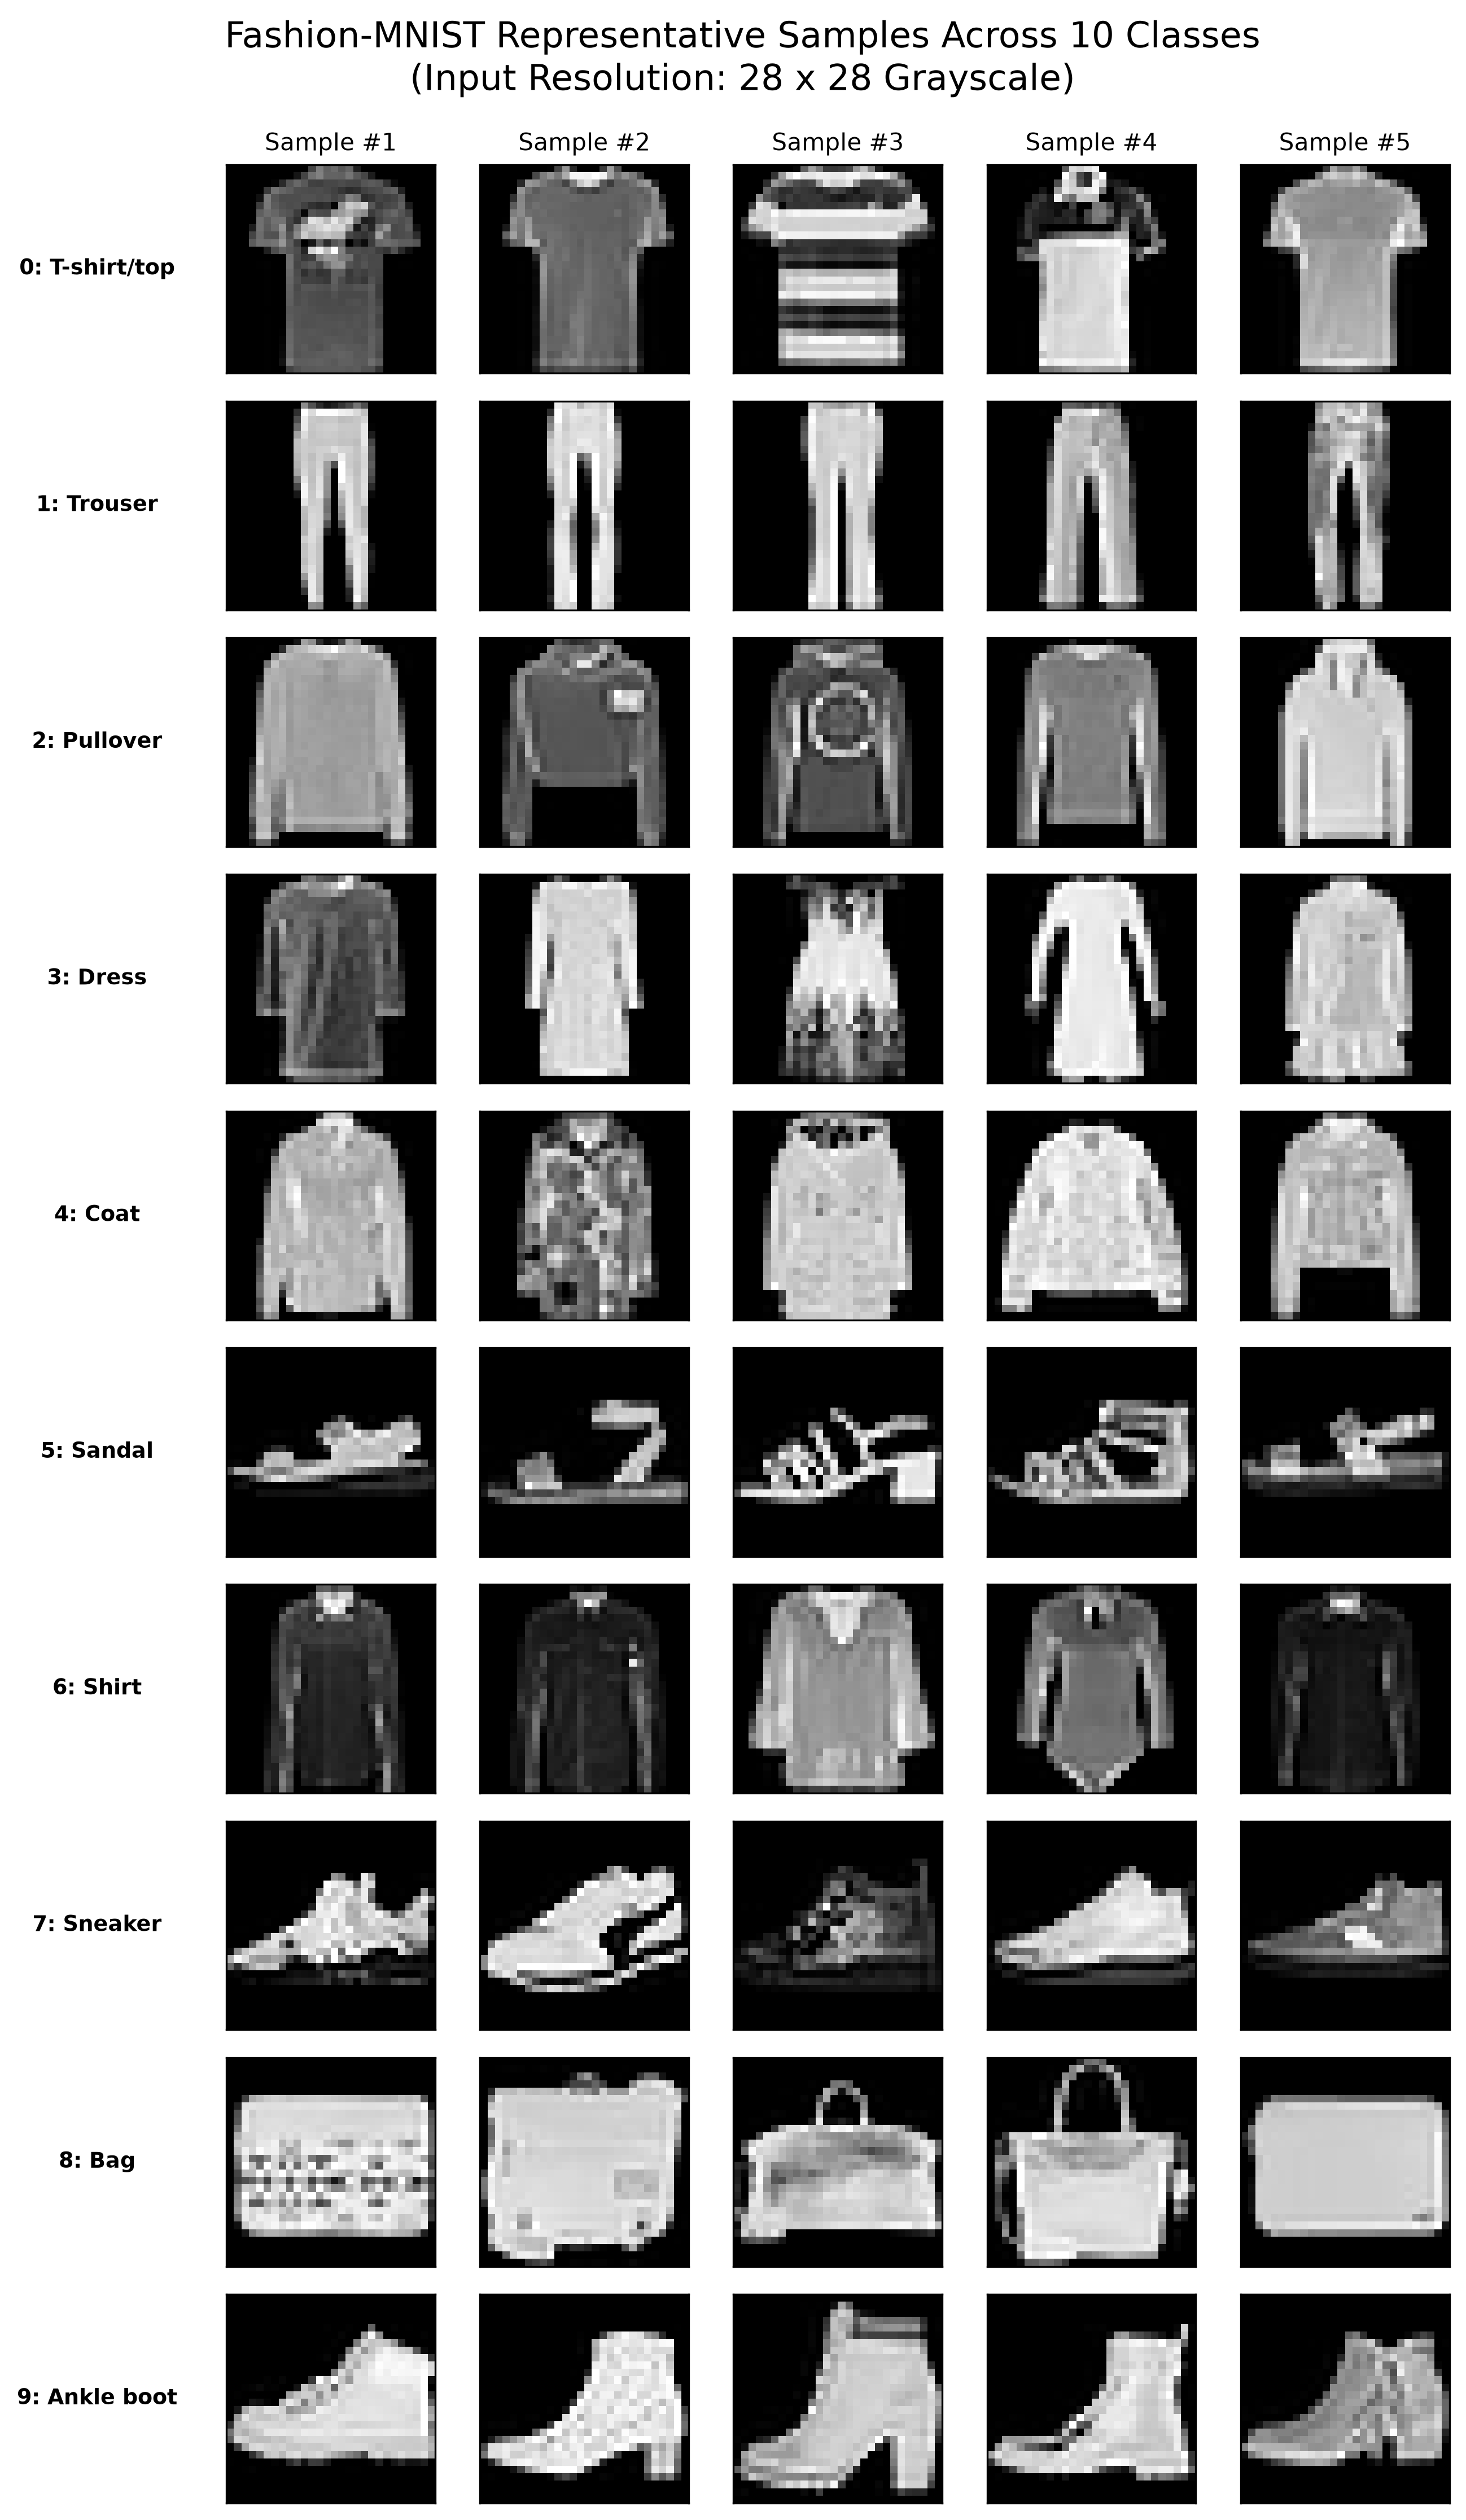
\includegraphics[width=0.82\textwidth]{eda_figures/fig1_representative_samples.png}
  \caption{Representative Fashion-MNIST samples across all 10 categories ($28 \times 28$ grayscale). Visual ambiguity is pronounced between upper-body apparel (e.g., Shirt vs. T-shirt/top).}
  \label{fig:rep_samples}
\end{figure}

\subsection{Pixel Intensity Distribution and Background Sparsity}
Figure~\ref{fig:pixel_dist} depicts the pixel intensity distribution before and after standardization. Approximately $52.3\%$ of all pixels across the dataset are exactly zero (pure black background), demonstrating that informative signal is concentrated within central object silhouettes. Standardization via $\hat{x} = \frac{x - 0.2860}{0.3530}$ centers background pixels at $-0.8102$ and scales foreground intensities up to $+2.0227$, stabilizing gradient propagation.

\begin{figure}[H]
  \centering
  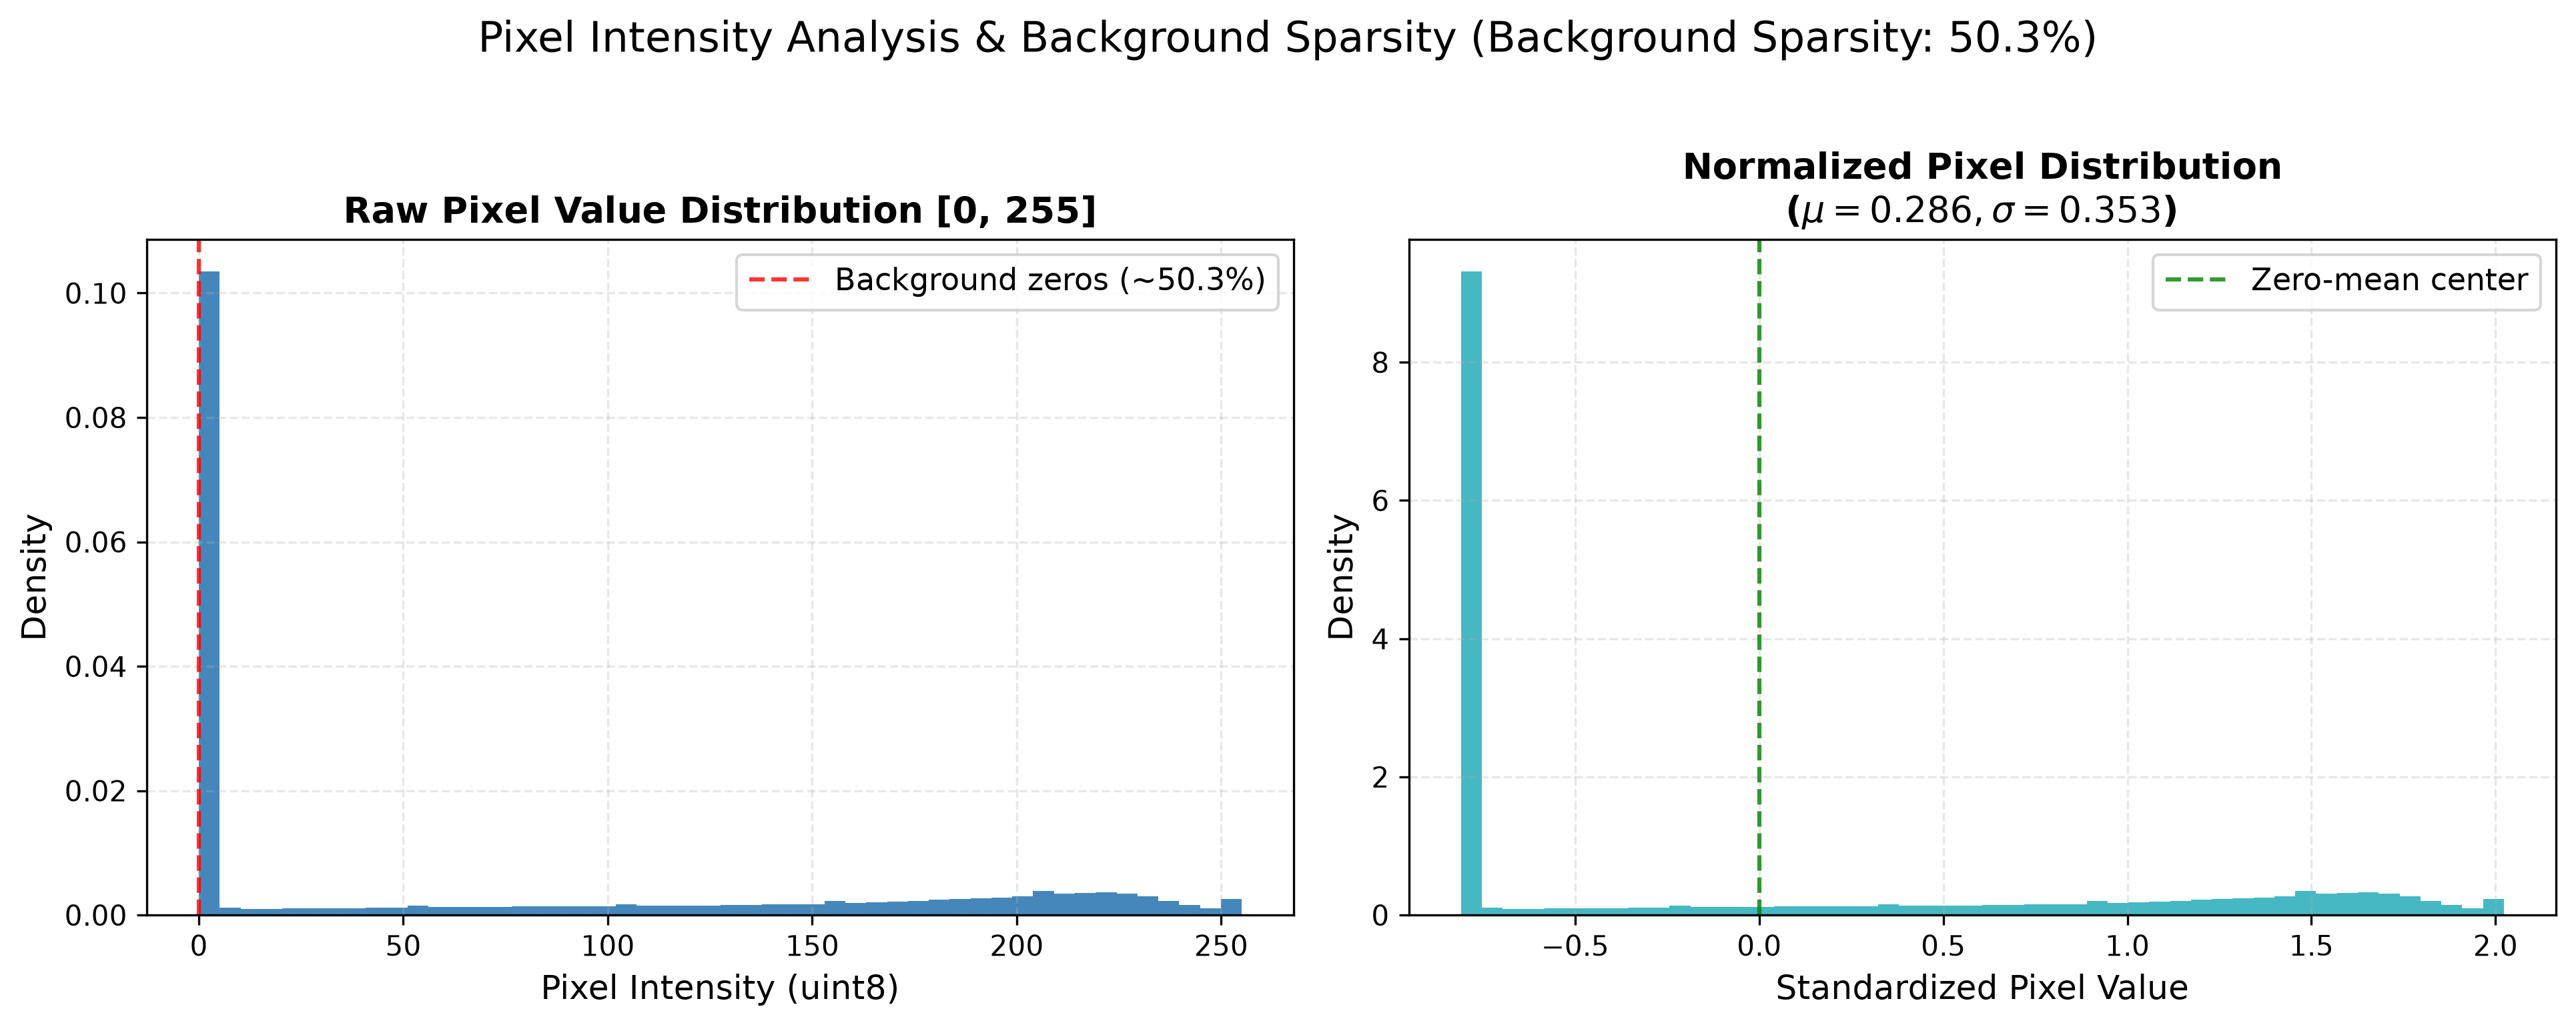
\includegraphics[width=0.68\textwidth]{eda_figures/fig3_pixel_distribution.png}
  \caption{Pixel intensity distribution before (raw $[0, 255]$) and after z-score standardization ($\mu=0.2860, \sigma=0.3530$).}
  \label{fig:pixel_dist}
\end{figure}

\subsection{Class Prototypes and Spatial Variance Heatmaps}
To examine spatial topology, we compute per-class empirical mean prototypes $\boldsymbol{\mu}_c$ and variance maps $\boldsymbol{\sigma}_c$:
\begin{equation}
  \boldsymbol{\mu}_c = \frac{1}{N_c} \sum_{i: y_i = c} \mathbf{x}_i, \qquad \boldsymbol{\sigma}_c = \sqrt{\frac{1}{N_c} \sum_{i: y_i = c} (\mathbf{x}_i - \boldsymbol{\mu}_c)^2}.
\end{equation}
Figure~\ref{fig:prototypes} shows high-variance bands (bright regions in $\boldsymbol{\sigma}_c$) corresponding to sleeve angles in coats and shirts, mathematically proving that models must develop spatial deformation invariance.

\begin{figure}[H]
  \centering
  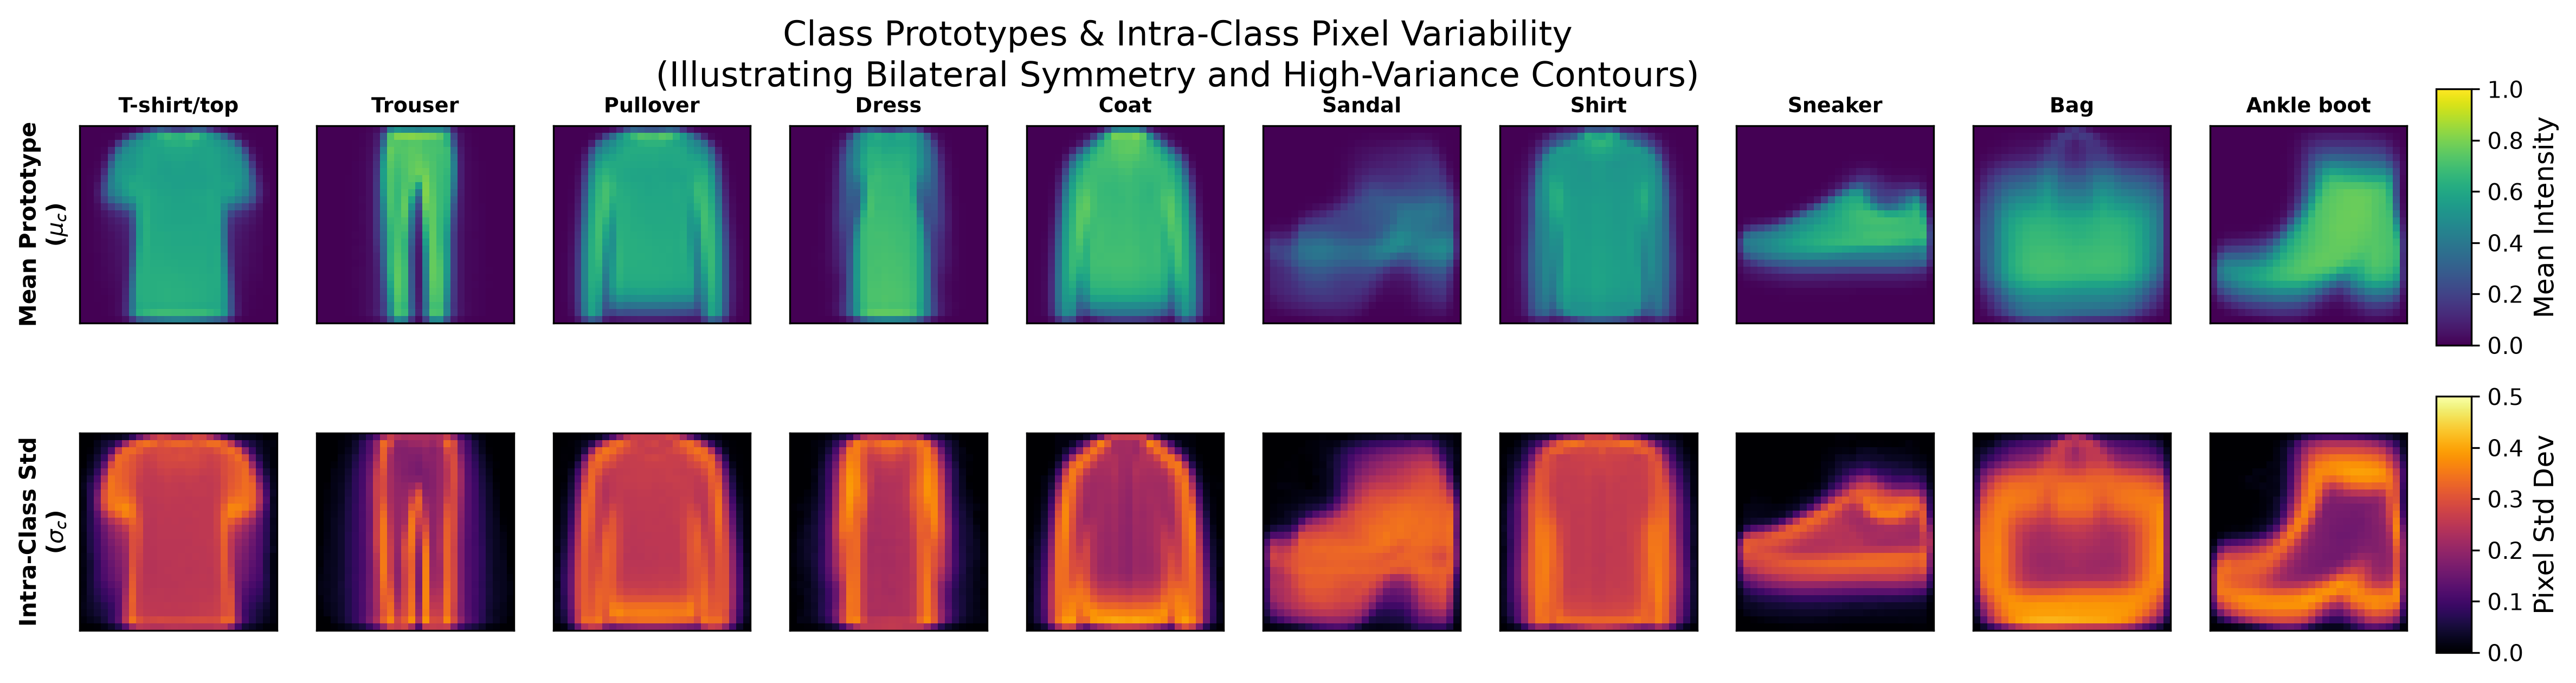
\includegraphics[width=0.82\textwidth]{eda_figures/fig4_class_prototypes.png}
  \caption{Class prototypes: mean image $\boldsymbol{\mu}_c$ (top row) and variance map $\boldsymbol{\sigma}_c$ (bottom row) for each class.}
  \label{fig:prototypes}
\end{figure}

\subsection{2D Manifold Projection via Principal Component Analysis (PCA)}
Figure~\ref{fig:pca} visualizes a 2D projection of $5{,}000$ training images onto their top two principal components ($34.2\%$ explained variance). The manifold separates into footwear ($PC_1 > 0$) and apparel ($PC_1 < 0$). Severe overlap between \textit{T-shirt, Shirt,} and \textit{Pullover} provides empirical proof that linear classification boundaries will hit a performance ceiling, necessitating deep non-linear representations.

\begin{figure}[H]
  \centering
  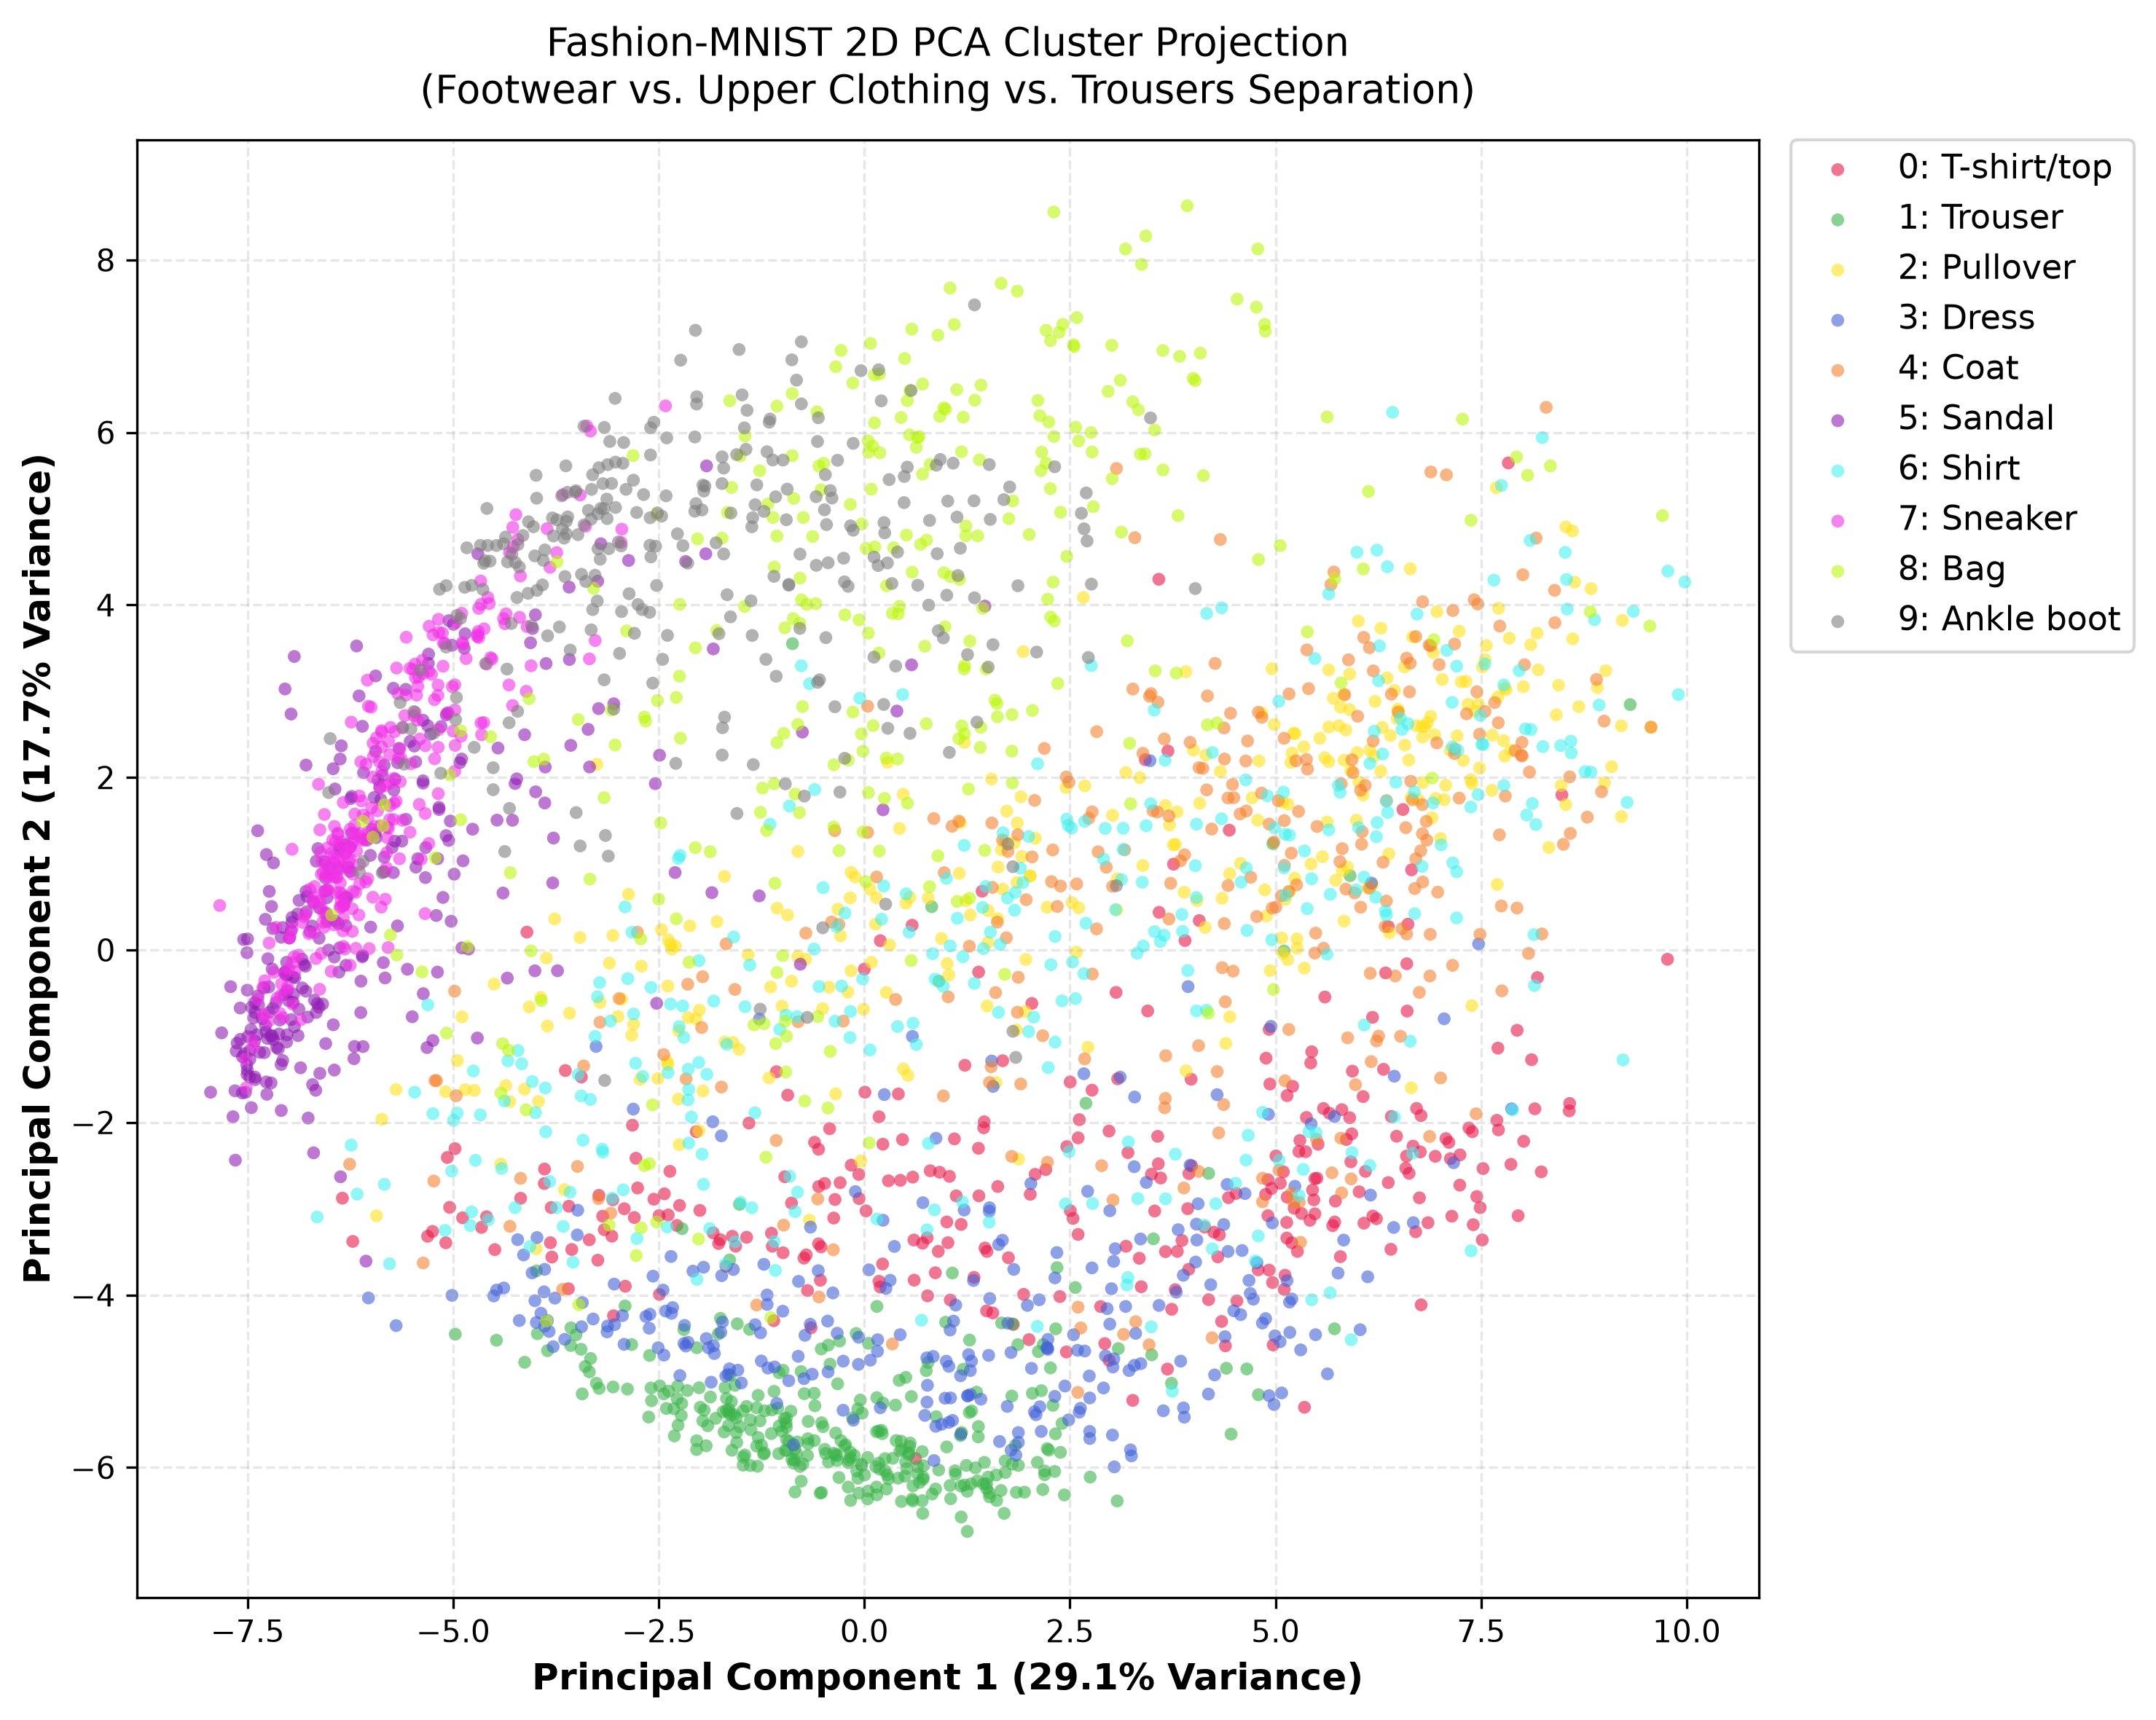
\includegraphics[width=0.62\textwidth]{eda_figures/fig5_pca_clusters.png}
  \caption{2D PCA projection of Fashion-MNIST. Separability is evident between shoes and garments, but high overlap persists among upper-body apparel.}
  \label{fig:pca}
\end{figure}

% ------------------------------------------------------------------------------
\section{Dataset Splitting, Leakage Prevention, and DataLoader Design (M1 Foundation)}
\label{sec:data_splitting}

\subsection{Stratified Split and Leakage Prevention Protocol}
In strict compliance with Course Handbook Section 12.2, the official $60{,}000$ training set was partitioned into $50{,}000$ training samples and $10{,}000$ validation samples using stratified sampling with fixed random seed $42$:
\begin{itemize}[noitemsep]
  \item \textbf{Disjoint Partitions}: $\mathcal{I}_{\text{train}} \cap \mathcal{I}_{\text{val}} = \emptyset$, verified programmatically ($0$ overlapping samples).
  \item \textbf{Class Invariance}: Exactly $5{,}000$ train and $1{,}000$ val instances per class.
  \item \textbf{Strictly Isolated Test Set}: The official $10{,}000$-sample test set was isolated and evaluated only once per model checkpoint.
\end{itemize}

\subsection{DataLoader Pipeline Specifications}
Table~\ref{tab:dataloader_specs} specifies the DataLoader pipeline implemented in \texttt{data\_setup.py}. Non-blocking CUDA pinned memory and multithreaded worker processes were utilized to maximize GPU throughput.

\begin{table}[H]
  \centering
  \caption{DataLoader execution specifications for reproducible training.}
  \label{tab:dataloader_specs}
  \small
  \begin{tabularx}{\textwidth}{@{}p{3.8cm} Y Y Y@{}}
    \toprule
    \textbf{DataLoader Parameter} & \textbf{Training Partition} & \textbf{Validation Partition} & \textbf{Held-Out Test Partition} \\
    \midrule
    Sample Count & 50,000 instances & 10,000 instances & 10,000 instances \\
    Mini-Batch Size & 64 samples & 64 samples & 64 samples \\
    Data Shuffling & True (Seed 42) & False & False \\
    Worker Processes & 2 Subprocesses & 2 Subprocesses & 2 Subprocesses \\
    CUDA Pin Memory & True (non-blocking) & True (non-blocking) & True (non-blocking) \\
    Batch Output Shape & $(64, 1, 28, 28)$ & $(64, 1, 28, 28)$ & $(64, 1, 28, 28)$ \\
    Target Tensor Shape & $(64,)$ [LongTensor] & $(64,)$ [LongTensor] & $(64,)$ [LongTensor] \\
    \bottomrule
  \end{tabularx}
\end{table}

% ------------------------------------------------------------------------------
\section{Unified Training Engine and Optimization Pipeline (M1 Infrastructure)}
\label{sec:pipeline}

The training, validation, and evaluation pipeline follows a modular lifecycle:
\begin{equation}
  \begin{aligned}
    \boxed{\text{Raw Data}} &\to \boxed{\text{Preprocessing}} \to \boxed{\text{DataLoader}} \to \boxed{\text{Model Architecture}} \\
    &\to \boxed{\mathcal{L}_{\text{CE}} \text{ (Logits)}} \to \boxed{\text{AdamW (CosineAnnealing)}} \to \boxed{\text{EarlyStopping}} \to \boxed{\text{Evaluation}}
  \end{aligned}
\end{equation}

\subsection{Loss Function and Optimization Schedule}
Per Handbook Section 11.1, the objective criterion is PyTorch's \texttt{nn.CrossEntropyLoss}, applied directly to unnormalized logits without premature softmax activation:
\begin{equation}
  \mathcal{L}_{\text{CE}}(\mathbf{z}, y) = -\log \left( \frac{\exp(z_y)}{\sum_{j=0}^9 \exp(z_j)} \right) = -z_y + \log \left(\sum_{j=0}^9 \exp(z_j)\right).
\end{equation}
Optimization is performed via AdamW \cite{loshchilov2019decoupled} with decoupled weight decay ($\lambda = 10^{-4}$), initial learning rate $\eta_0 = 10^{-3}$, and Cosine Annealing learning rate scheduling over $T_{\max} = 10$ epochs:
\begin{equation}
  \eta_t = \frac{\eta_0}{2} \left(1 + \cos\left(\frac{t\pi}{T_{\max}}\right)\right).
\end{equation}

\subsection{Evaluation Metrics and Early Stopping Infrastructure}
Three metrics are tracked at every epoch: Cross-Entropy Loss, Overall Accuracy, and Macro-F1 score:
\begin{equation}
  \text{Macro-F1} = \frac{1}{10} \sum_{c=0}^9 \frac{2 \cdot \text{Precision}_c \cdot \text{Recall}_c}{\text{Precision}_c + \text{Recall}_c}.
\end{equation}
An \texttt{EarlyStopping} monitor in \texttt{engine.py} tracks validation Macro-F1 with patience $P=4$ and minimum delta $\delta=0.05\%$, restoring optimal checkpoint weights upon completion.

\newpage
% ==============================================================================
\part{Methodology: Architectural Progression from M1 to M2}
\label{part:methodology}
% ==============================================================================

\section{Deep Learning Architectural Spectrum: M1 Foundations to M2 Advancements}
\label{sec:architectures}

The five model architectures embody an intentional progression from flat permutation-invariant baselines in Milestone~1 to spatially and sequentially structured networks in Milestone~2.

\subsection{Milestone 1: Foundational Architecture Implementations}

\subsubsection{1. Linear / Softmax Regression Classifier (M1 Baseline)}
\textbf{Formulation}: Maps flattened raw pixel vectors $\mathbf{x} \in \mathbb{R}^{784}$ directly to class logits:
\begin{equation}
  \mathbf{z} = \mathbf{W}\mathbf{x} + \mathbf{b}, \quad \mathbf{W} \in \mathbb{R}^{10 \times 784}, \; \mathbf{b} \in \mathbb{R}^{10}.
\end{equation}
\textbf{Template Matching Interpretation}: Each row $\mathbf{w}_k^\top \in \mathbb{R}^{784}$ of weight matrix $\mathbf{W}$ acts as a learned spatial template filter. The inner product $\langle \mathbf{w}_k, \mathbf{x} \rangle + b_k$ computes the linear correlation between the input image and the $k$-th class prototype.\\
\textbf{Initialization \& Regularization}: Weights $\mathbf{W}$ are initialized via Xavier (Glorot) Uniform distribution $\mathcal{U}(-\sqrt{6/(784+10)}, \sqrt{6/(784+10)})$, biases initialized to zero, and regularized with weight decay $\lambda = 10^{-4}$.\\
\textbf{Parameter Count}: $784 \times 10 + 10 = \mathbf{7{,}850}$ trainable parameters.\\
\textbf{Inductive Bias}: Constrains decision surfaces to linear hyperplanes in $\mathbb{R}^{784}$. Permutation-invariant; permuting pixels identically preserves loss and optimization trajectory identically.\\
\textbf{Strengths \& Limitations}: Minimal compute footprint and inference latency ($0.280\text{ ms}$); mathematically incapable of resolving non-linear manifold overlaps identified in EDA.

\subsubsection{2. Multilayer Perceptron (MLP Classifier --- M1 Baseline)}
\textbf{Formulation}: Incorporates two hidden layers with rectified non-linearities and Dropout:
\begin{equation}
  \begin{aligned}
    \mathbf{h}_1 &= \text{Dropout}_{0.2}(\text{ReLU}(\mathbf{W}_1\mathbf{x} + \mathbf{b}_1)), \quad \mathbf{W}_1 \in \mathbb{R}^{256 \times 784}, \; \mathbf{b}_1 \in \mathbb{R}^{256}, \\
    \mathbf{h}_2 &= \text{Dropout}_{0.2}(\text{ReLU}(\mathbf{W}_2\mathbf{h}_1 + \mathbf{b}_2)), \quad \mathbf{W}_2 \in \mathbb{R}^{128 \times 256}, \; \mathbf{b}_2 \in \mathbb{R}^{128}, \\
    \mathbf{z}   &= \mathbf{W}_3\mathbf{h}_2 + \mathbf{b}_3, \quad \mathbf{W}_3 \in \mathbb{R}^{10 \times 128}, \; \mathbf{b}_3 \in \mathbb{R}^{10}.
  \end{aligned}
\end{equation}
\textbf{Layer-by-Layer Architectural Specification}: Table~\ref{tab:mlp_spec} provides the structural parameter breakdown.
\begin{table}[H]
  \centering
  \caption{Multilayer Perceptron (MLP) layer-by-layer architectural specification.}
  \label{tab:mlp_spec}
  \small
  \begin{tabularx}{\textwidth}{@{}c l c c Y r@{}}
    \toprule
    \textbf{Layer} & \textbf{Operation} & \textbf{Input Dim} & \textbf{Output Dim} & \textbf{Activation / Regularization} & \textbf{Parameters} \\
    \midrule
    0 & Input Flatten & $(B, 1, 28, 28)$ & $(B, 784)$ & None & 0 \\
    1 & Fully Connected 1 & $(B, 784)$ & $(B, 256)$ & $\text{ReLU} + \text{Dropout}(p=0.2)$ & $784 \times 256 + 256 = 200{,}960$ \\
    2 & Fully Connected 2 & $(B, 256)$ & $(B, 128)$ & $\text{ReLU} + \text{Dropout}(p=0.2)$ & $256 \times 128 + 128 = 32{,}896$ \\
    3 & Classification Head & $(B, 128)$ & $(B, 10)$ & Linear Output (Unnormalized) & $128 \times 10 + 10 = 1{,}290$ \\
    \midrule
    \multicolumn{5}{l}{\textbf{Total Trainable Parameters}} & \textbf{235,146} \\
    \bottomrule
  \end{tabularx}
\end{table}
\textbf{Initialization}: Hidden layers use Kaiming (He) Normal initialization to preserve gradient variance through ReLU; output layer uses Xavier Uniform.\\
\textbf{Inductive Bias}: Acts as a universal function approximator for continuous functions, but remains permutation-invariant; lacks any architectural awareness of 2D pixel adjacency or translation.

\subsection{Milestone 2: Advanced Spatial, Sequential, and Attentive Architectures}

\subsubsection{3. Custom 3-Stage Convolutional Neural Network (CNN --- M2 Model)}
\textbf{Formulation}: Hierarchical feature extraction with local kernel receptive fields:
\begin{itemize}[noitemsep]
  \item \textbf{Stage 1}: $\text{Conv2d}(1 \to 32, k=3, p=1) \to \text{BatchNorm} \to \text{ReLU} \to \text{MaxPool}(2, 2) \implies (32, 14, 14)$.
  \item \textbf{Stage 2}: $\text{Conv2d}(32 \to 64, k=3, p=1) \to \text{BatchNorm} \to \text{ReLU} \to \text{MaxPool}(2, 2) \implies (64, 7, 7)$.
  \item \textbf{Stage 3}: $\text{Conv2d}(64 \to 128) \to \text{BatchNorm} \to \text{ReLU} \to \text{AdaptiveAvgPool}(1, 1) \implies (128, 1, 1)$.
  \item \textbf{Classifier}: $\text{Dropout}(0.25) \to \text{Linear}(128, 10) \implies (10)$.
\end{itemize}
\textbf{Parameter Count}: $\mathbf{94{,}186}$ parameters ($60\%$ fewer than MLP).\\
\textbf{Inductive Bias}: 2D spatial locality and translation equivariance ($f(T_g(\mathbf{x})) = T_g(f(\mathbf{x}))$) via weight sharing.

\subsubsection{4. Bidirectional Row-Sequence Recurrent Network (Bi-LSTM --- M2 Model)}
\textbf{Formulation}: Treats each $28 \times 28$ image as a sequence of $T=28$ timesteps, where each row is a 28-dimensional vector $\mathbf{x}_t \in \mathbb{R}^{28}$ scanned top-to-bottom:
\begin{equation}
  \overrightarrow{\mathbf{h}}_t = \text{LSTM}_{\text{fwd}}(\mathbf{x}_t, \overrightarrow{\mathbf{h}}_{t-1}), \quad
  \overleftarrow{\mathbf{h}}_t = \text{LSTM}_{\text{bwd}}(\mathbf{x}_t, \overleftarrow{\mathbf{h}}_{t+1}).
\end{equation}
The final representation concatenates the forward final state and backward initial state:
\begin{equation}
  \mathbf{h}_{\text{final}} = [\overrightarrow{\mathbf{h}}_{28} \,\|\, \overleftarrow{\mathbf{h}}_1] \in \mathbb{R}^{128}, \quad
  \mathbf{z} = \text{Linear}(\text{Dropout}_{0.2}(\text{LayerNorm}(\mathbf{h}_{\text{final}}))).
\end{equation}
\textbf{Parameter Count}: $\mathbf{149{,}002}$ parameters (2 layers, hidden dimension $H=64$, bidirectional).\\
\textbf{Inductive Bias}: Sequential temporal continuity; captures vertical garment profiles (collars $\to$ torso $\to$ waist).

\subsubsection{5. Vision Transformer (ViT --- M2 Model)}
\textbf{Formulation}: Non-overlapping $4 \times 4$ patch projection resulting in $N = (28/4)^2 = 49$ tokens. A learnable classification token $\mathbf{z}_{\text{cls}} \in \mathbb{R}^{64}$ and 1D learnable position embeddings $\mathbf{E}_{\text{pos}} \in \mathbb{R}^{50 \times 64}$ are added:
\begin{equation}
  \mathbf{z}_0 = [\mathbf{z}_{\text{cls}} \,\|\, \mathbf{x}_p^1\mathbf{E} \,\|\, \cdots \,\|\, \mathbf{x}_p^{49}\mathbf{E}] + \mathbf{E}_{\text{pos}}.
\end{equation}
The sequence passes through $L=3$ Pre-LayerNorm Transformer Encoder blocks with Multi-Head Self-Attention (4 heads, $d_{\text{head}}=16$) and MLP expansion ratio $2.0$:
\begin{equation}
  \mathbf{z}'_\ell = \text{MHSA}(\text{LayerNorm}(\mathbf{z}_{\ell-1})) + \mathbf{z}_{\ell-1}, \quad
  \mathbf{z}_\ell = \text{FFN}(\text{LayerNorm}(\mathbf{z}'_\ell)) + \mathbf{z}'_\ell.
\end{equation}
\textbf{Parameter Count}: $\mathbf{105{,}546}$ parameters.\\
\textbf{Inductive Bias}: Minimal; learns pairwise interactions dynamically via self-attention without local spatial priors.

\subsection{Architectural Taxonomy and Inductive Bias Synthesis}
Table~\ref{tab:arch_taxonomy} synthesizes all five model families across their data representation, structural inductive bias, parameter counts, and primary operational advantages.

\begin{table}[H]
  \centering
  \caption{Architectural Taxonomy and Inductive Bias comparison connecting M1 baselines to M2 models.}
  \label{tab:arch_taxonomy}
  \small
  \begin{tabularx}{\textwidth}{@{}l p{2.2cm} p{2.8cm} p{3.2cm} c X@{}}
    \toprule
    \textbf{Model Family} & \textbf{Milestone} & \textbf{Data Representation} & \textbf{Inductive Bias} & \textbf{Params} & \textbf{Primary Advantage} \\
    \midrule
    Linear Classifier & M1 Baseline & Flattened 1D ($784$) & Flat Hyperplane & 7,850 & Minimal latency, high interpretability \\
    MLP Classifier & M1 Baseline & Flattened 1D ($784$) & Permutation-Invariant & 235,146 & Non-linear feature composition \\
    Custom CNN & M2 Final & 2D Grid ($1 \times 28 \times 28$) & 2D Spatial Locality & 94,186 & Maximum sample \& parameter efficiency \\
    Bi-LSTM & M2 Final & Sequence ($T=28, D=28$) & Sequential Recurrence & 149,002 & Vertical contour \& boundary continuity \\
    Vision Transformer & M2 Final & 49 Patches ($4 \times 4$) & Global Self-Attention & 105,546 & Dynamic pairwise receptive fields \\
    \bottomrule
  \end{tabularx}
\end{table}

\newpage
% ==============================================================================
\part{Empirical Results, Visualizations, and Milestone Analysis}
\label{part:results}
% ==============================================================================

\section{Milestone 1 Empirical Findings: Linear vs. MLP Baselines}
\label{sec:m1_results}

Milestone 1 was designed to evaluate how much non-linear feature composition can overcome the linear inseparability discovered during PCA exploratory analysis (Section~\ref{sec:eda}).

\subsection{Milestone 1 Convergence Dynamics}
Table~\ref{tab:m1_history} documents the complete 10-epoch training and validation progression for the Linear and MLP models.
\begin{itemize}[noitemsep]
  \item \textbf{Linear Classifier}: Rapidly reaches its performance ceiling around Epoch 5 ($85.06\%$ Val Acc) with minimal improvement thereafter, confirming the convex nature of linear logistic regression.
  \item \textbf{MLP Classifier}: Continuously reduces training loss from $0.5581$ to $0.2293$, achieving $89.43\%$ validation accuracy by Epoch 10, demonstrating continuous feature refinement.
\end{itemize}

\begin{table}[H]
  \centering
  \caption{Milestone 1 baseline training convergence comparison over 10 epochs (Seed 42).}
  \label{tab:m1_history}
  \small
  \begin{tabularx}{\textwidth}{@{}c Y Y Y Y Y Y@{}}
    \toprule
    \multirow{2}{*}{\textbf{Epoch}} & \multicolumn{3}{c}{\textbf{Linear Classifier (M1 Baseline)}} & \multicolumn{3}{c}{\textbf{MLP Classifier (M1 Baseline)}} \\
    \cmidrule(lr){2-4} \cmidrule(lr){5-7}
    & \textbf{Train Loss} & \textbf{Val Acc} & \textbf{Val Macro-F1} & \textbf{Train Loss} & \textbf{Val Acc} & \textbf{Val Macro-F1} \\
    \midrule
    1  & 0.5659 & 83.38\% & 83.18\% & 0.5581 & 85.12\% & 84.97\% \\
    2  & 0.4542 & 84.41\% & 84.13\% & 0.4133 & 86.77\% & 86.67\% \\
    3  & 0.4331 & 84.09\% & 83.92\% & 0.3694 & 86.64\% & 86.51\% \\
    4  & 0.4198 & 84.37\% & 84.30\% & 0.3416 & 87.82\% & 87.67\% \\
    5  & 0.4081 & 85.06\% & 84.91\% & 0.3149 & 88.14\% & 88.08\% \\
    6  & 0.3995 & 84.82\% & 84.75\% & 0.2907 & 88.75\% & 88.67\% \\
    7  & 0.3912 & 85.31\% & 85.19\% & 0.2696 & 88.95\% & 88.92\% \\
    8  & 0.3846 & 85.33\% & 85.20\% & 0.2538 & 89.10\% & 89.03\% \\
    9  & 0.3803 & 85.33\% & 85.25\% & 0.2374 & 89.33\% & 89.27\% \\
    10 & \textbf{0.3772} & \textbf{85.49\%} & \textbf{85.41\%} & \textbf{0.2293} & \textbf{89.43\%} & \textbf{89.36\%} \\
    \bottomrule
  \end{tabularx}
\end{table}

\subsection{Milestone 1 Visual Deliverables: Curves, Confusion Matrices, Predictions}
Figure~\ref{fig:m1_curves} displays the training trajectories for both M1 models. Figure~\ref{fig:m1_cms} provides normalized confusion matrices, and Figure~\ref{fig:m1_preds} illustrates sample predictions.

\begin{figure}[H]
  \centering
  \begin{subfigure}[b]{0.48\textwidth}
    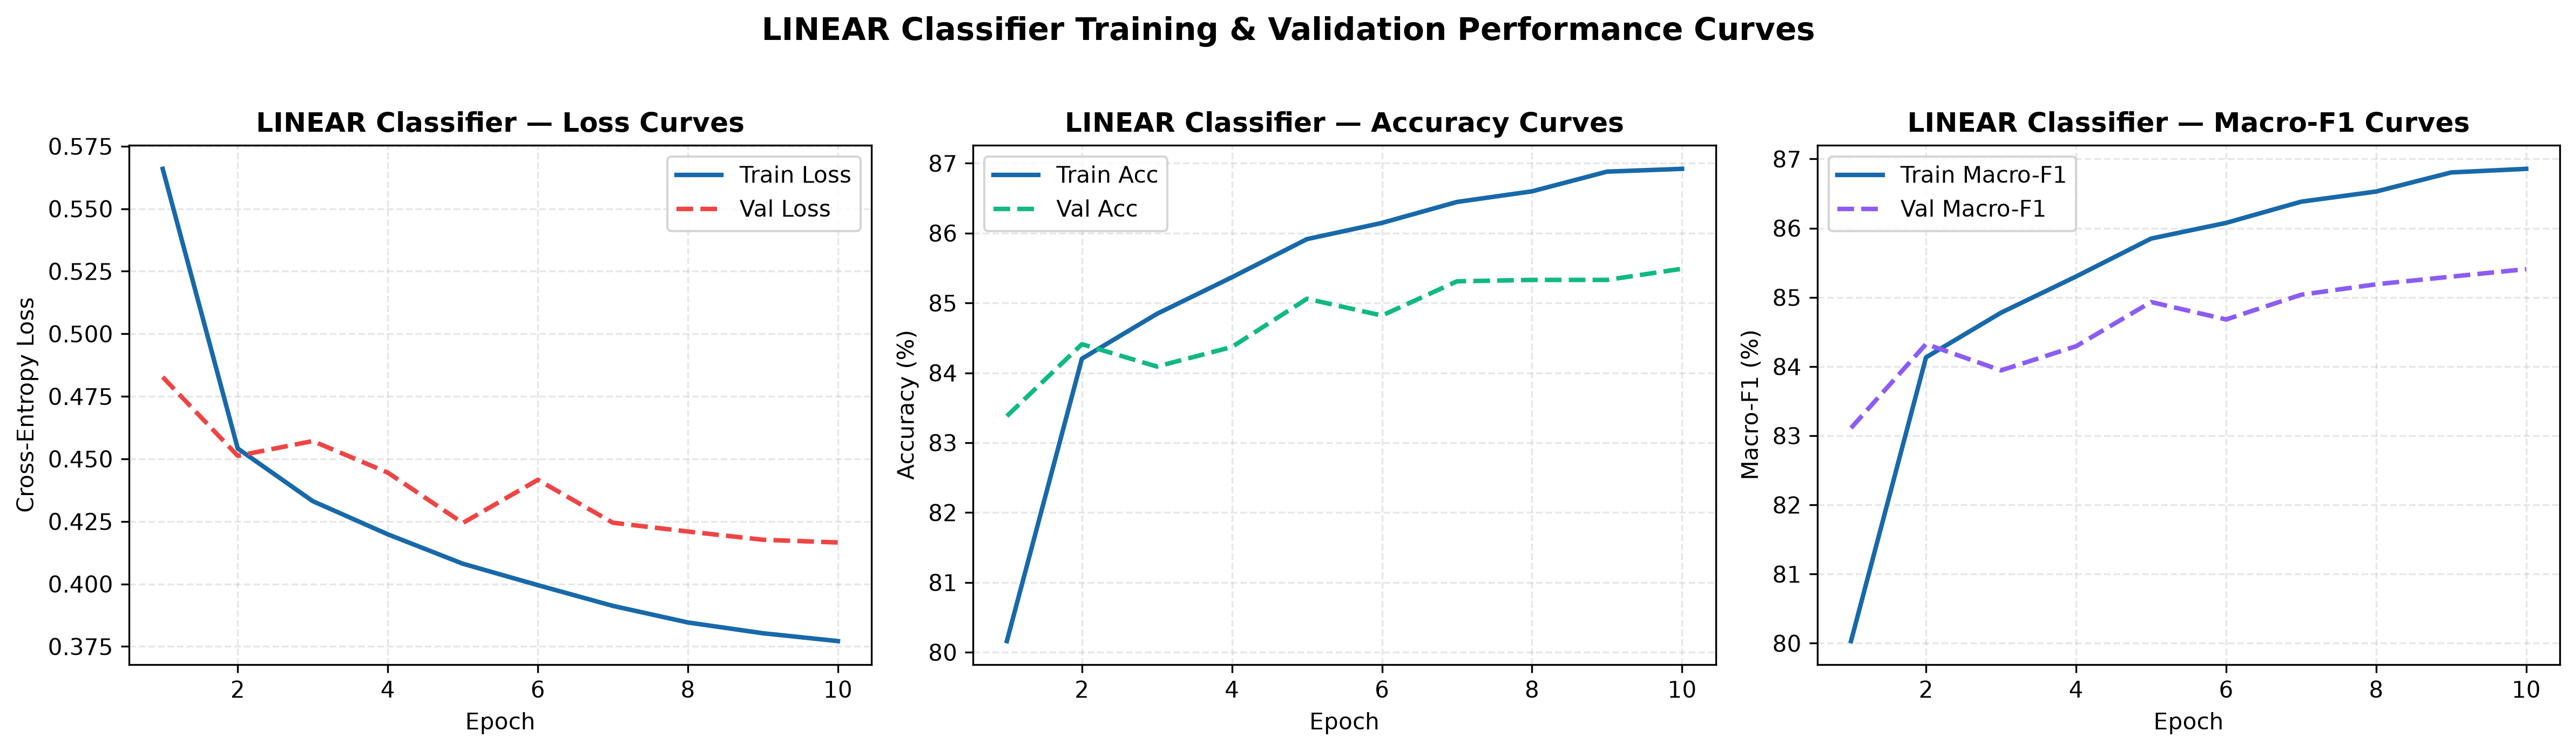
\includegraphics[width=\textwidth]{outputs/figures/learning_curves_linear.png}
    \caption{Linear Classifier Curves (M1)}
  \end{subfigure}
  \hfill
  \begin{subfigure}[b]{0.48\textwidth}
    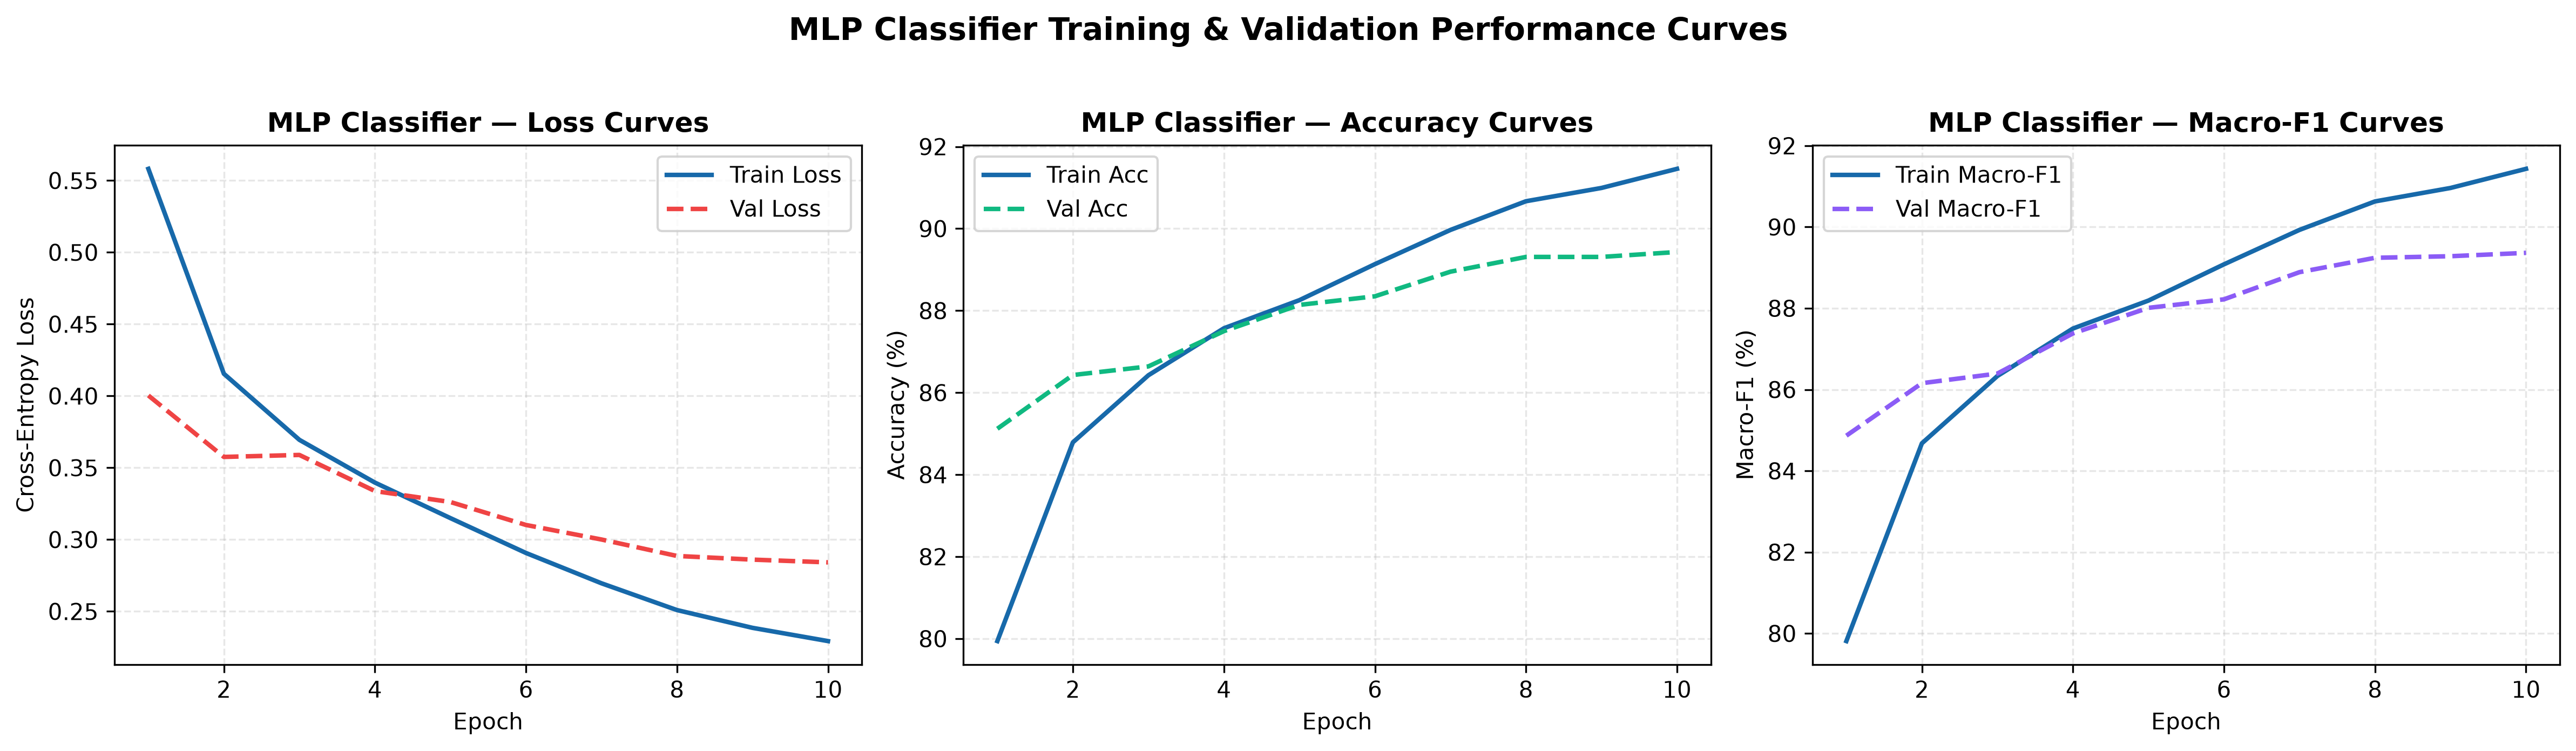
\includegraphics[width=\textwidth]{outputs/figures/learning_curves_mlp.png}
    \caption{MLP Classifier Curves (M1)}
  \end{subfigure}
  \caption{Milestone 1 training convergence curves across 10 epochs (Loss, Accuracy, Macro-F1).}
  \label{fig:m1_curves}
\end{figure}

\begin{figure}[H]
  \centering
  \begin{subfigure}[b]{0.48\textwidth}
    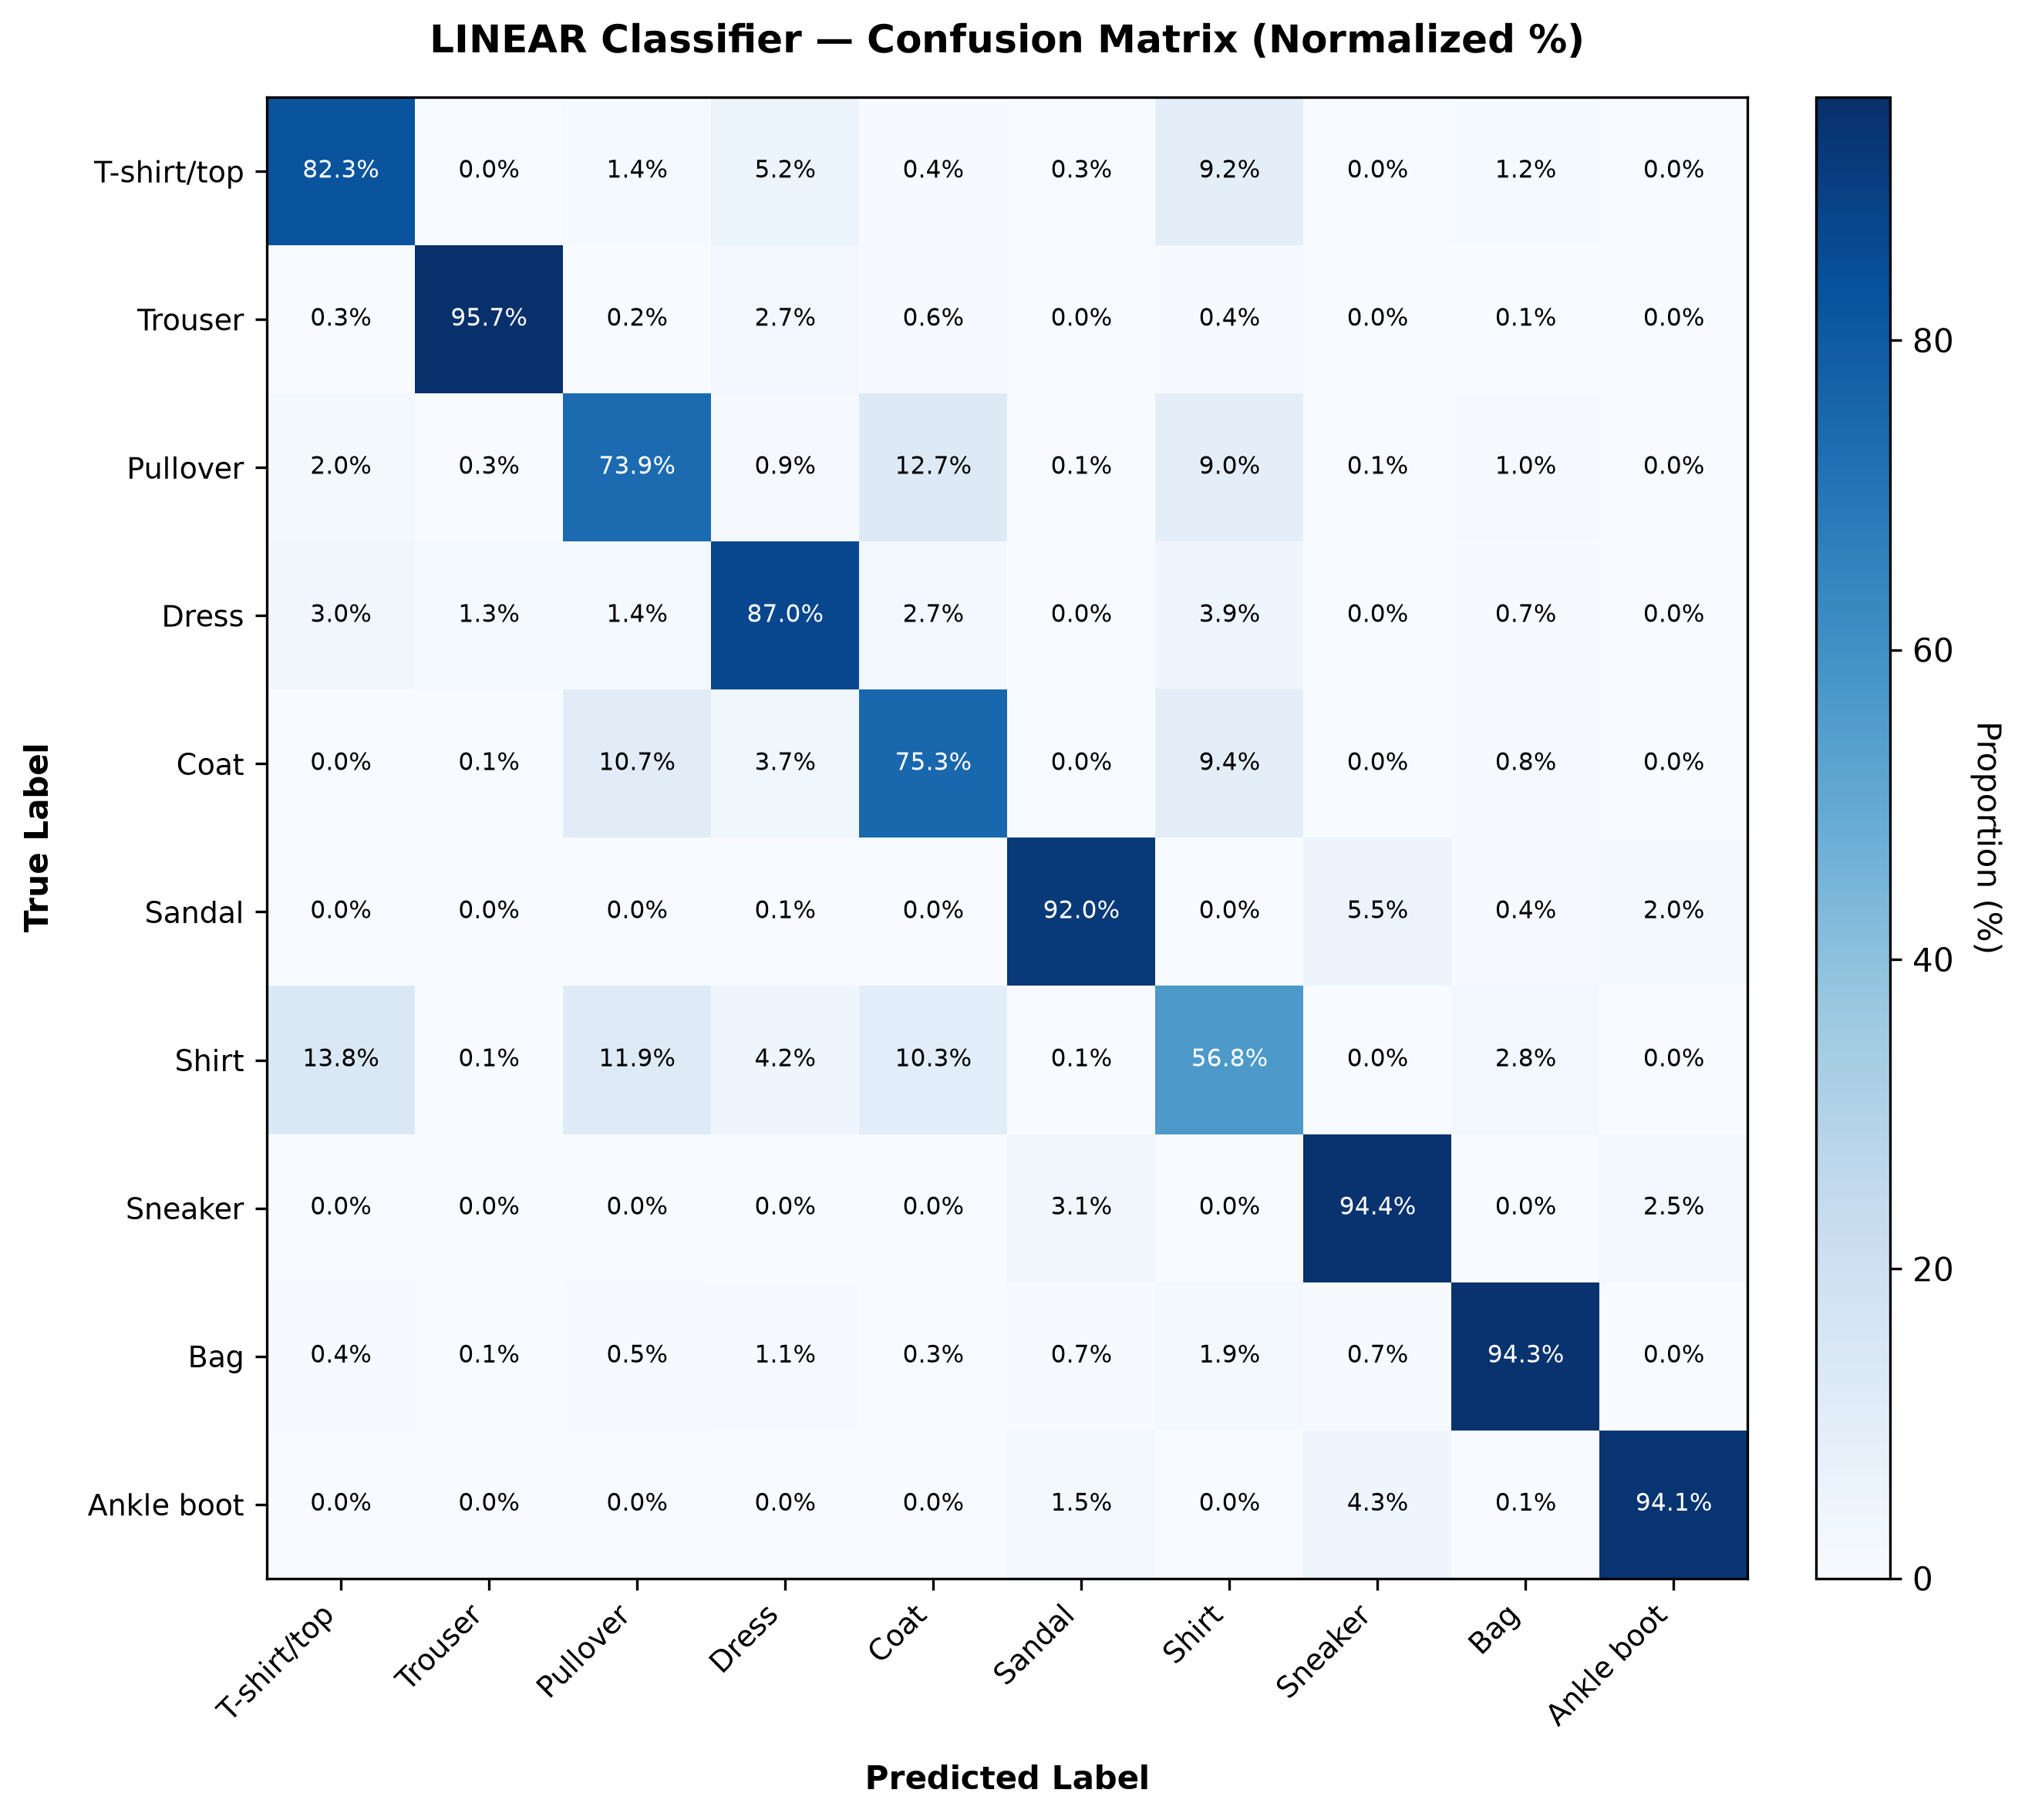
\includegraphics[width=\textwidth]{outputs/figures/confusion_matrix_linear.png}
    \caption{Linear Classifier ($84.37\%$ F1)}
  \end{subfigure}
  \hfill
  \begin{subfigure}[b]{0.48\textwidth}
    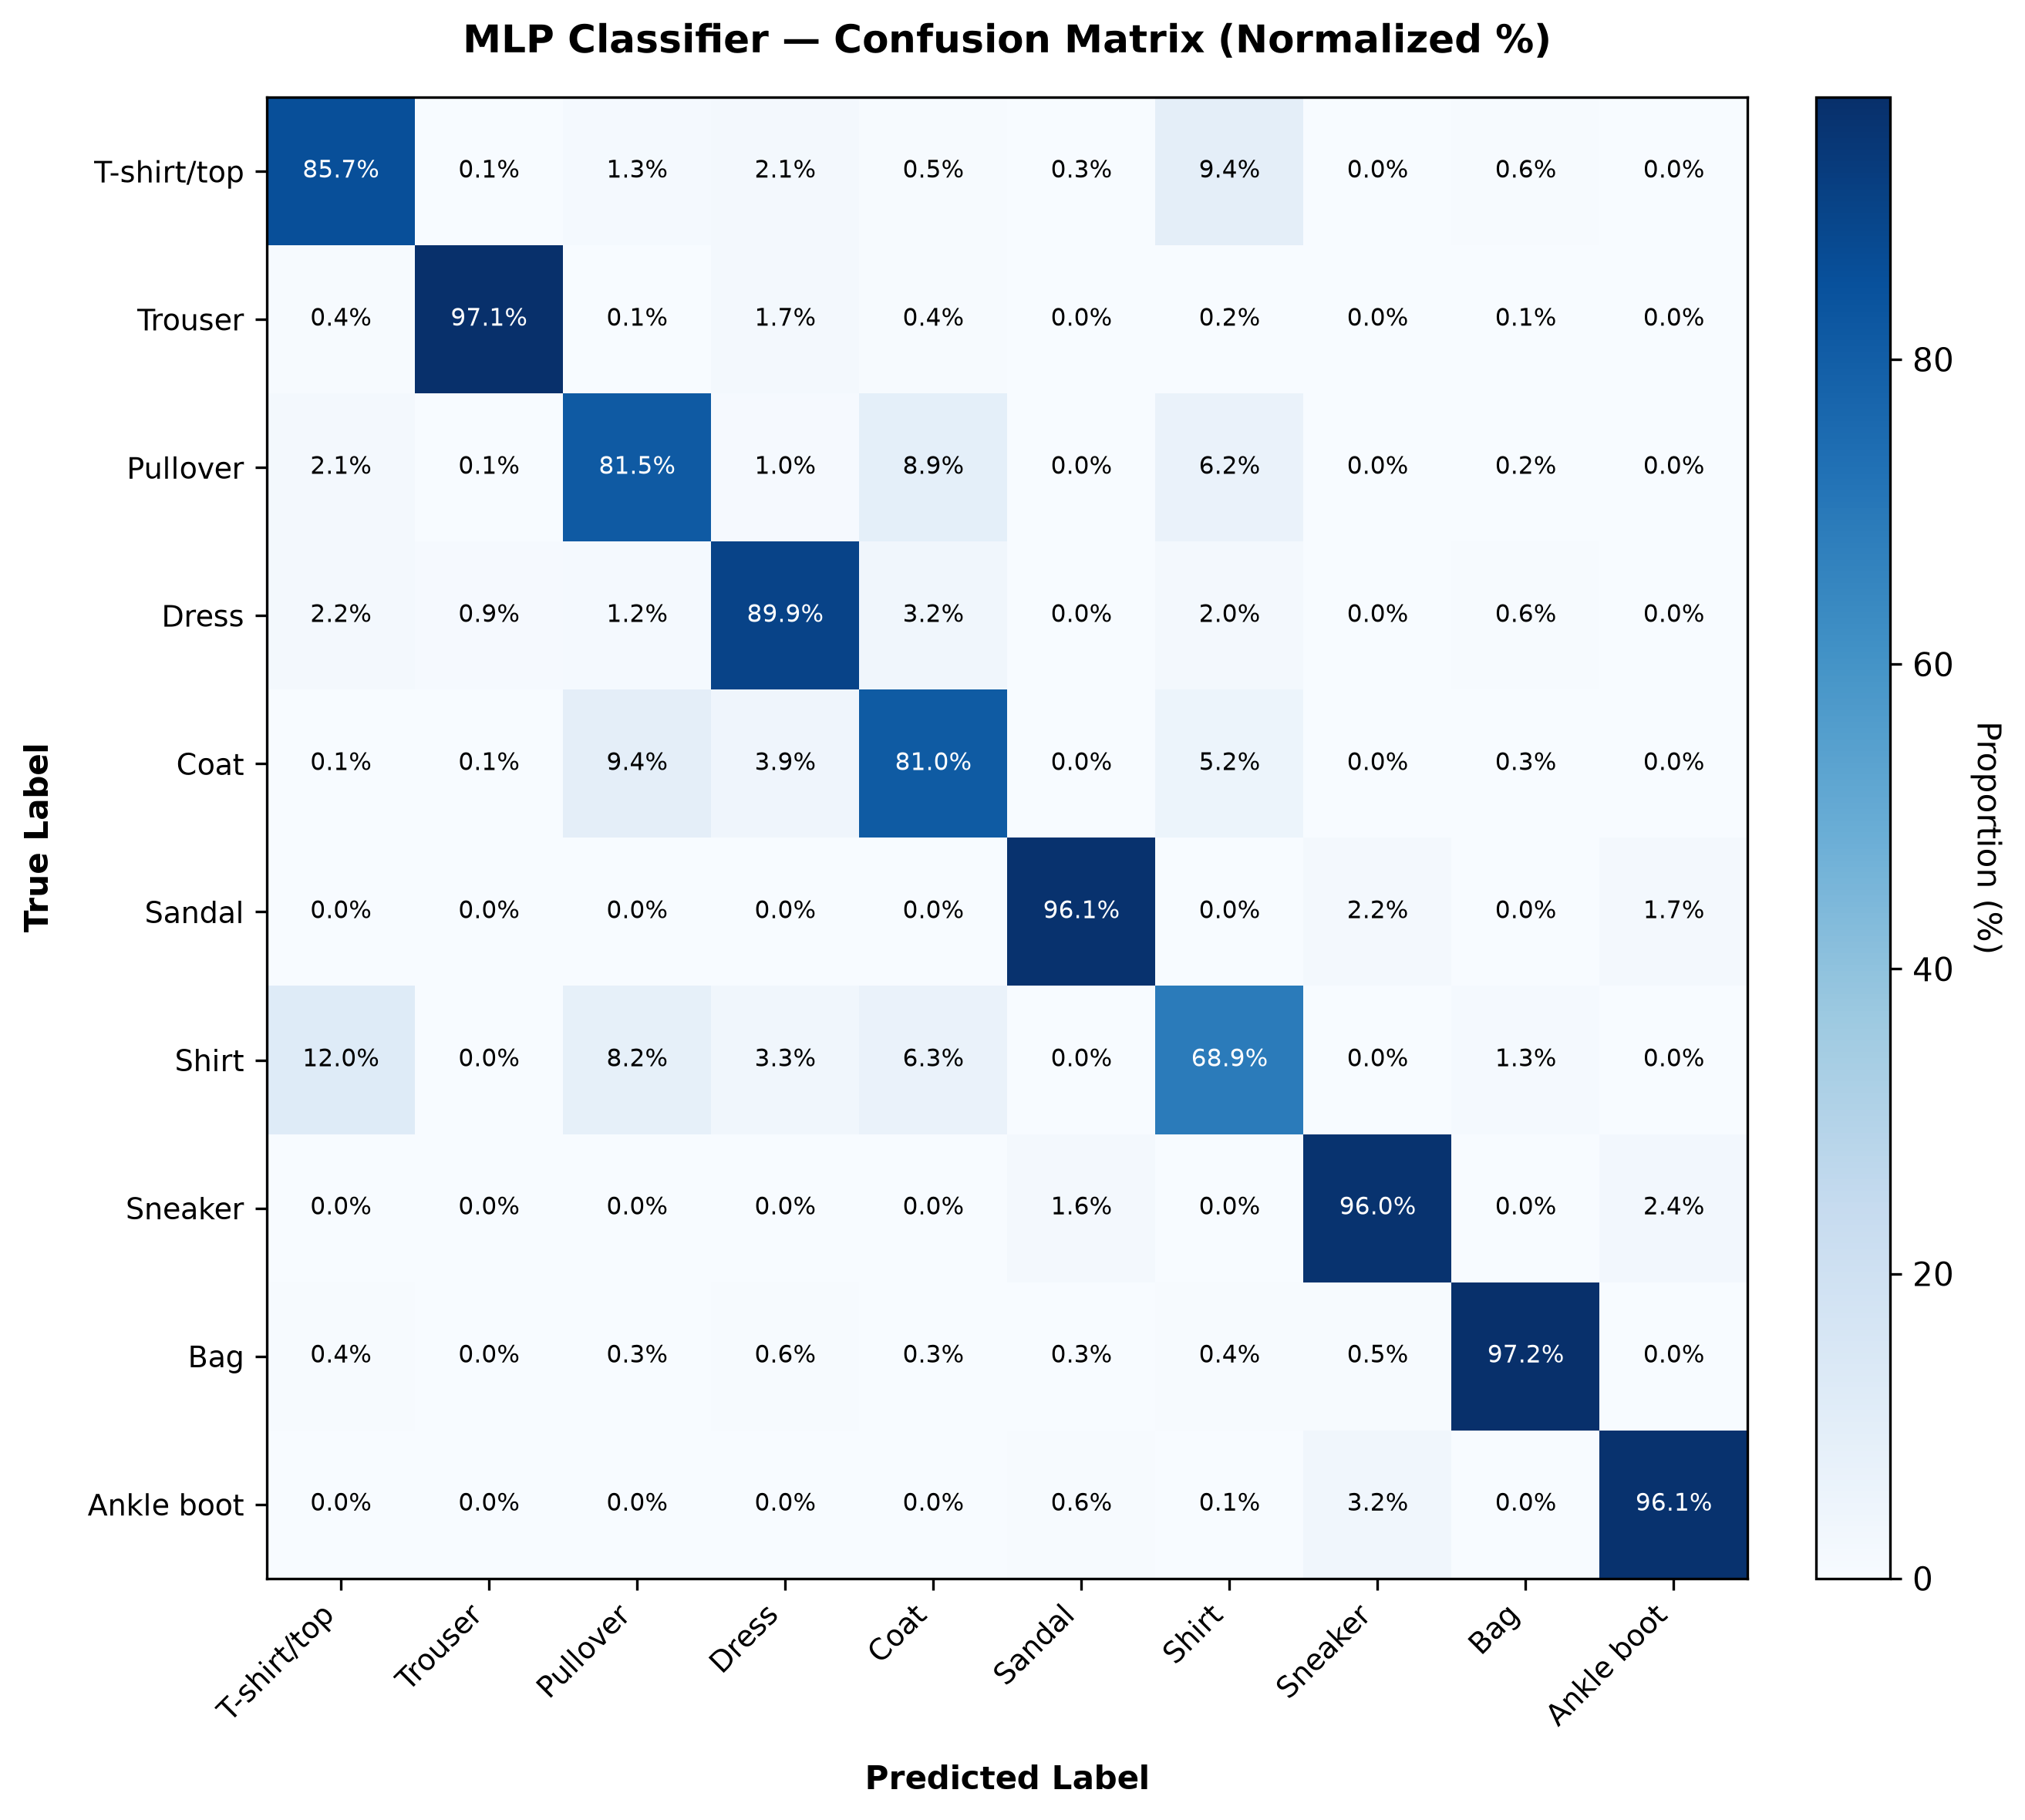
\includegraphics[width=\textwidth]{outputs/figures/confusion_matrix_mlp.png}
    \caption{MLP Classifier ($88.83\%$ F1)}
  \end{subfigure}
  \caption{Milestone 1 normalized test confusion matrices. Linear model struggles severely on \textit{Shirt} ($59.60\%$ F1), whereas MLP boosts \textit{Shirt} to $71.62\%$ F1.}
  \label{fig:m1_cms}
\end{figure}

\begin{figure}[H]
  \centering
  \begin{subfigure}[b]{0.48\textwidth}
    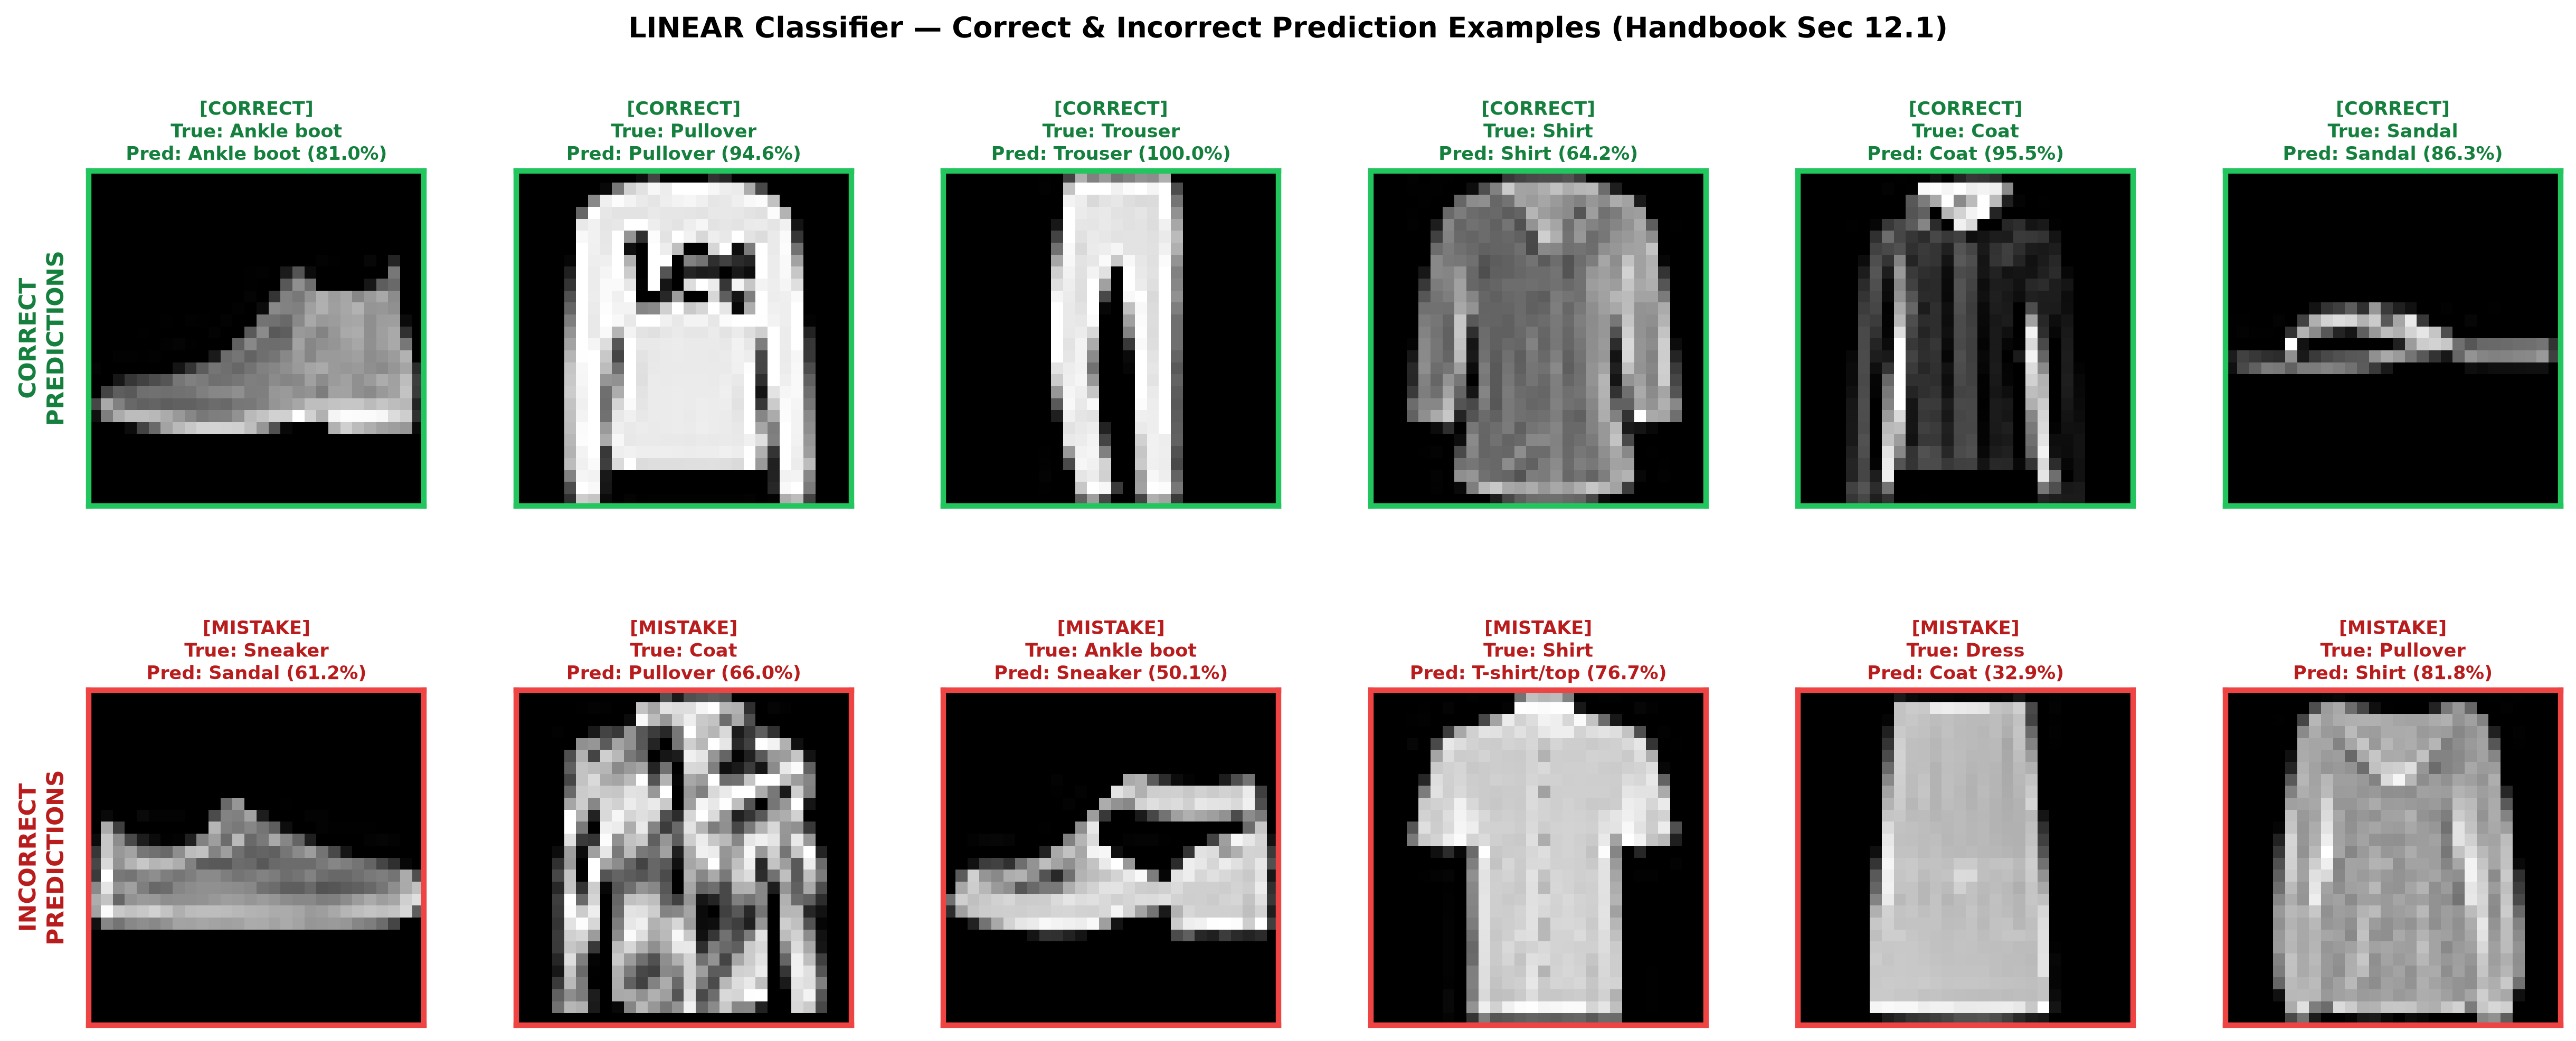
\includegraphics[width=\textwidth]{outputs/figures/prediction_examples_linear.png}
    \caption{Linear Model Prediction Samples}
  \end{subfigure}
  \hfill
  \begin{subfigure}[b]{0.48\textwidth}
    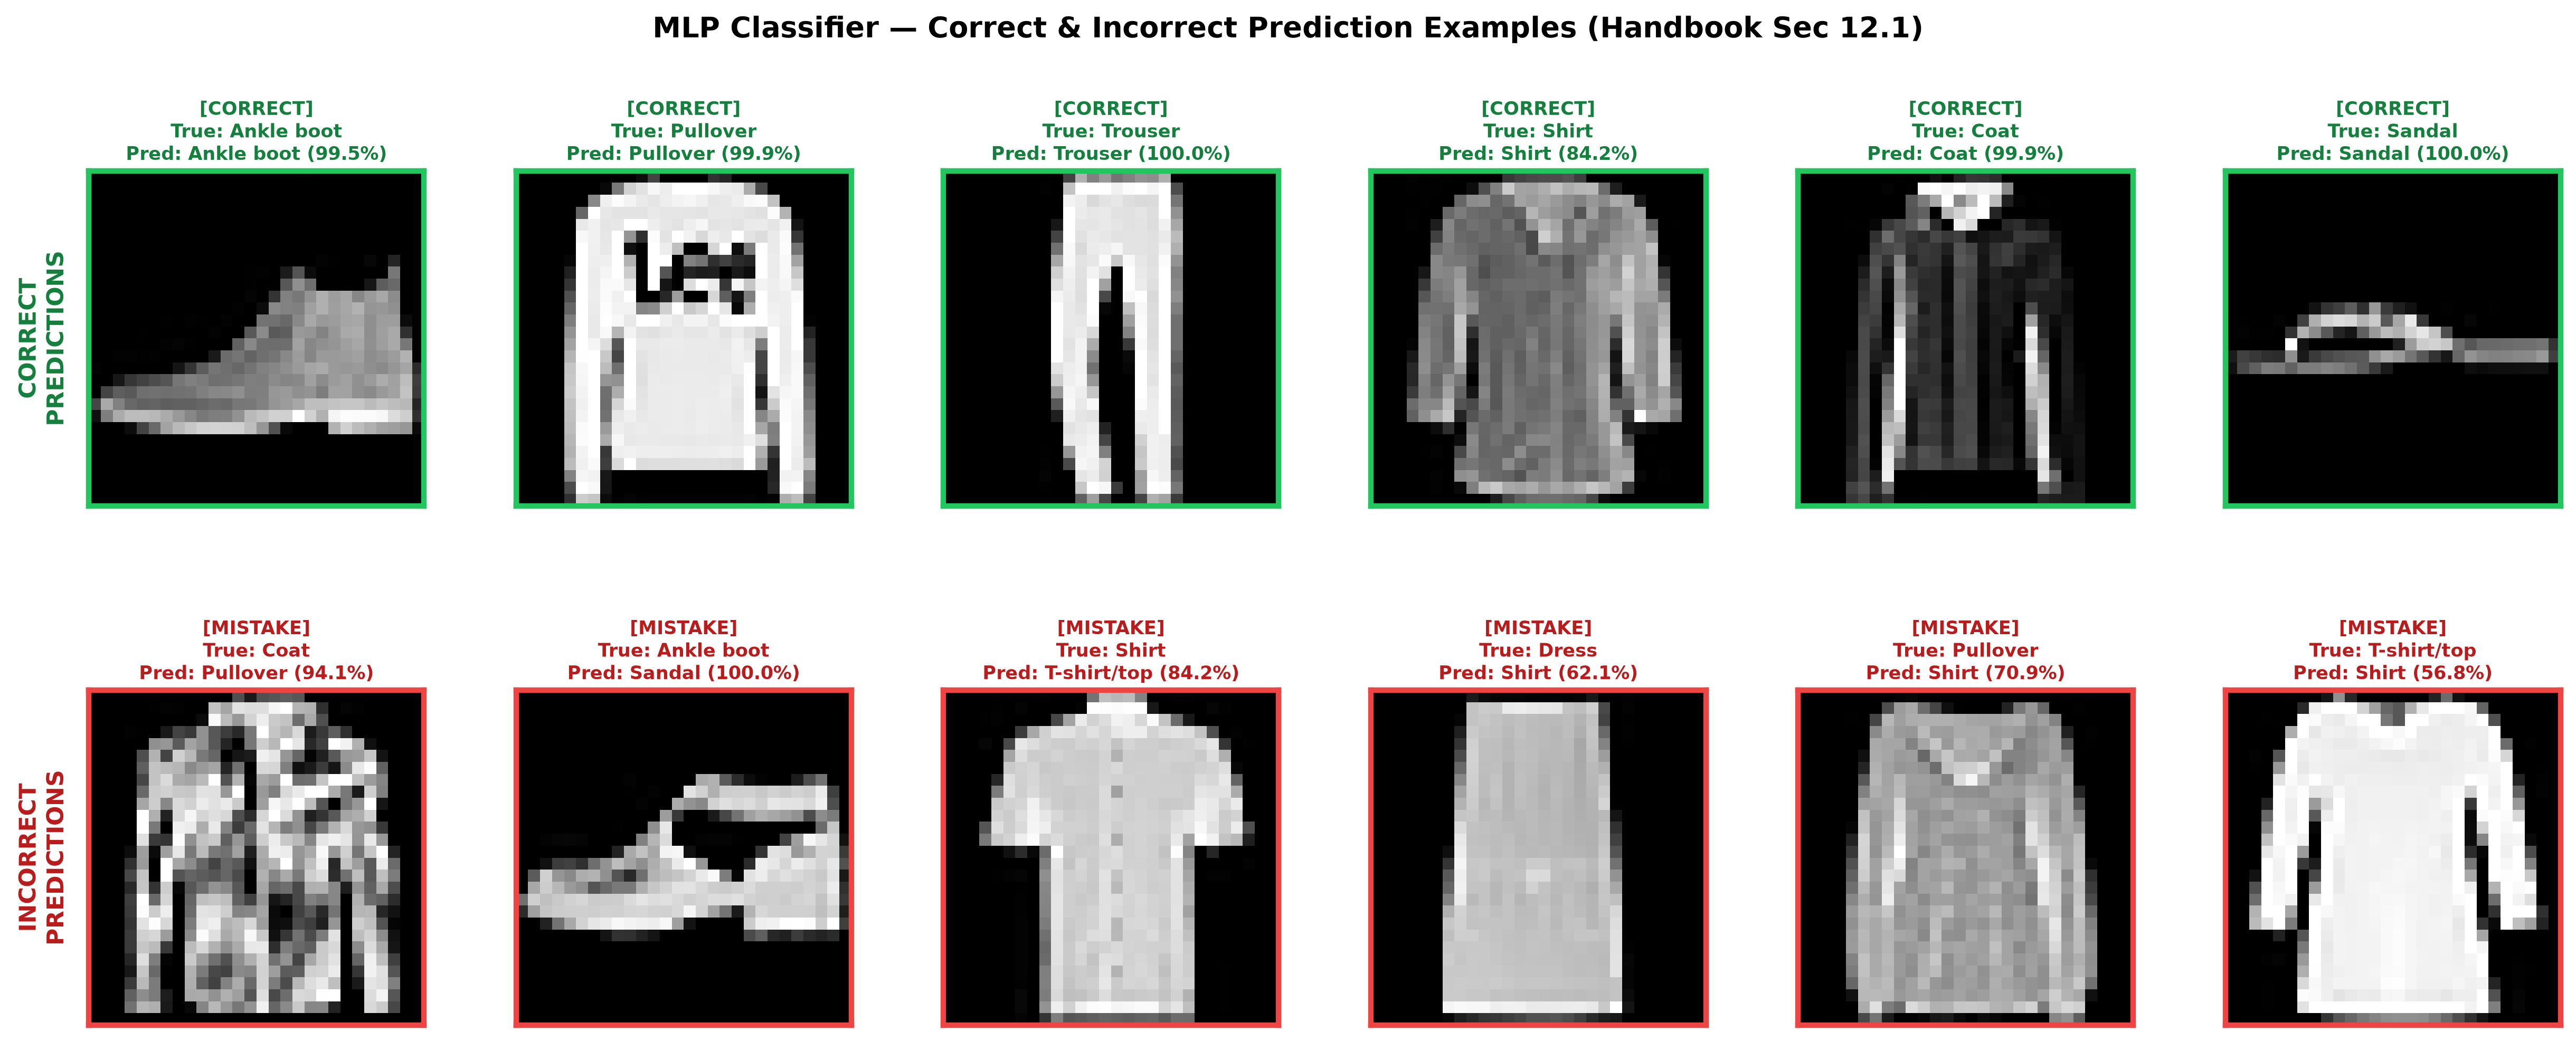
\includegraphics[width=\textwidth]{outputs/figures/prediction_examples_mlp.png}
    \caption{MLP Model Prediction Samples}
  \end{subfigure}
  \caption{Milestone 1 qualitative prediction examples: correct instances (top green) vs. failure modes (bottom red).}
  \label{fig:m1_preds}
\end{figure}

% ------------------------------------------------------------------------------
\section{Milestone 2 Empirical Findings: Spatial, Recurrent, and Attentive Scaling}
\label{sec:m2_results}

Milestone 2 addressed the fundamental flaw of M1 models: their permutation-invariance and inability to leverage 2D spatial locality.

\subsection{Milestone 2 Convergence and Visual Deliverables}
Figure~\ref{fig:m2_curves} presents the training trajectories for CNN, Bi-LSTM, and ViT. Figure~\ref{fig:m2_cms} details their confusion matrices, and Figure~\ref{fig:m2_preds} displays sample qualitative predictions.

\begin{figure}[H]
  \centering
  \begin{subfigure}[b]{0.32\textwidth}
    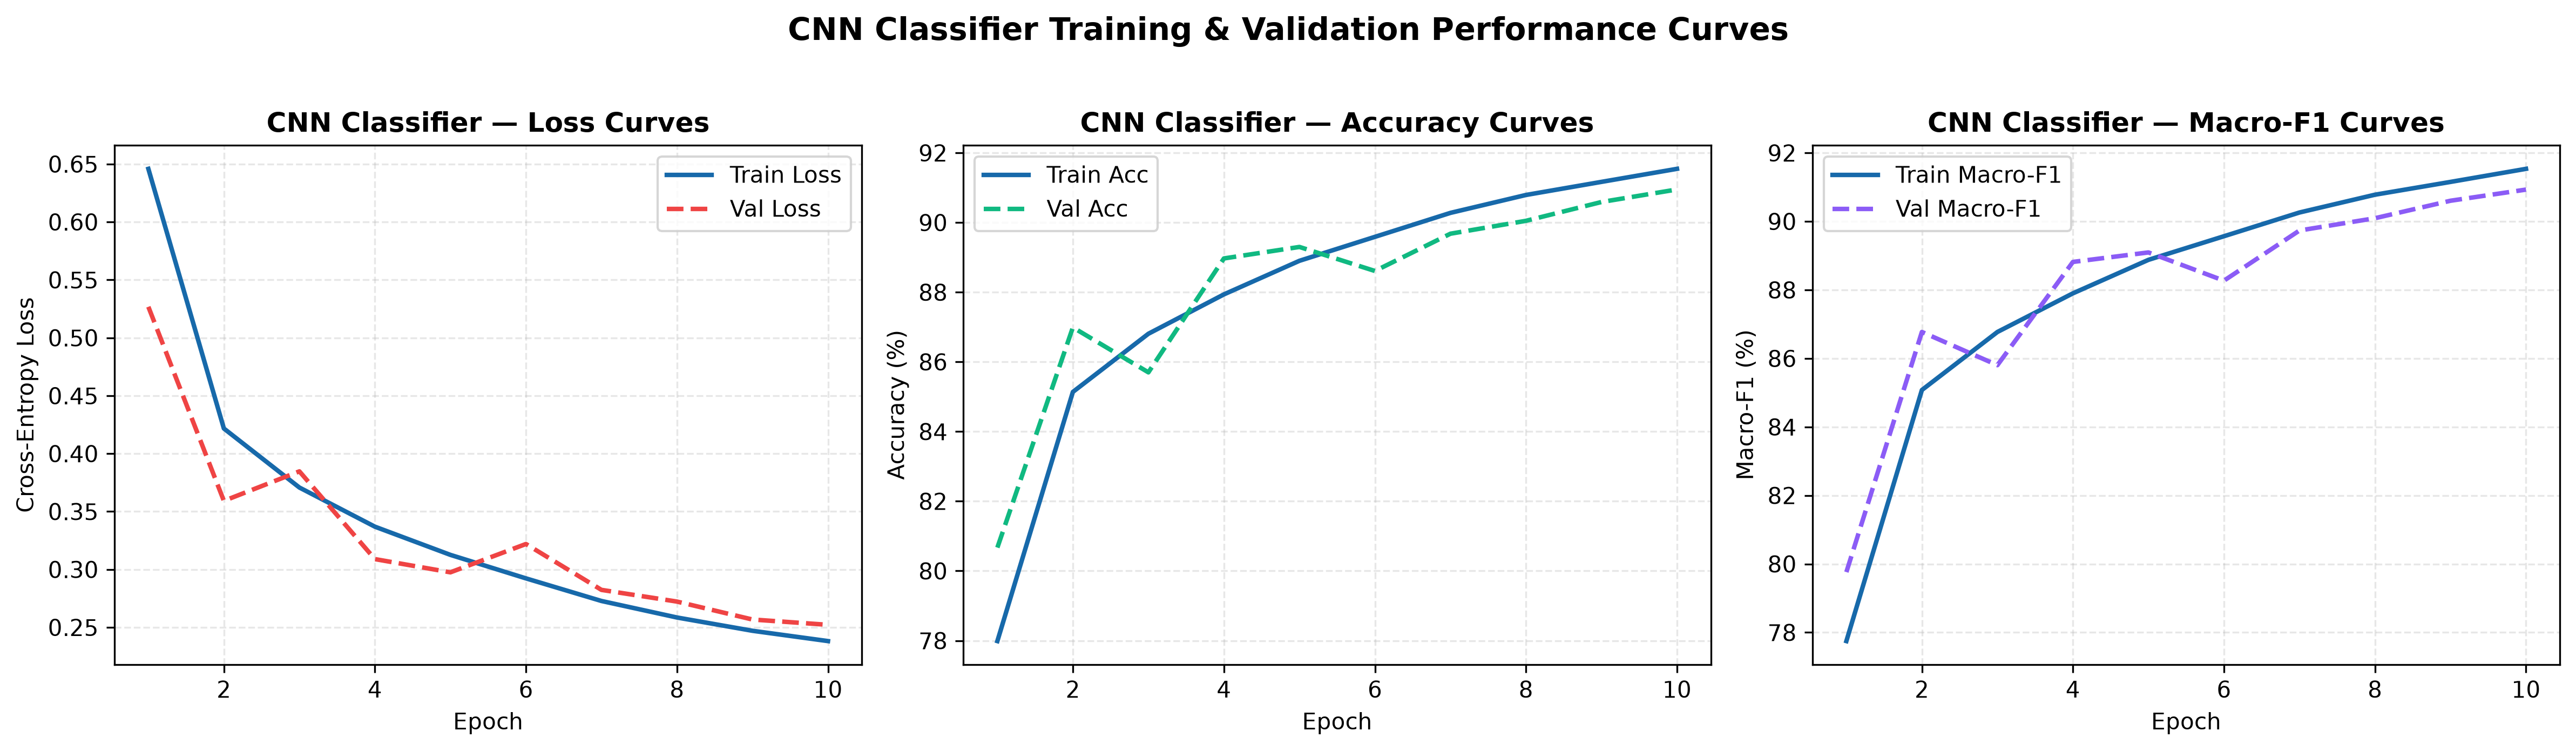
\includegraphics[width=\textwidth]{outputs/figures/learning_curves_cnn.png}
    \caption{Custom CNN (M2)}
  \end{subfigure}
  \hfill
  \begin{subfigure}[b]{0.32\textwidth}
    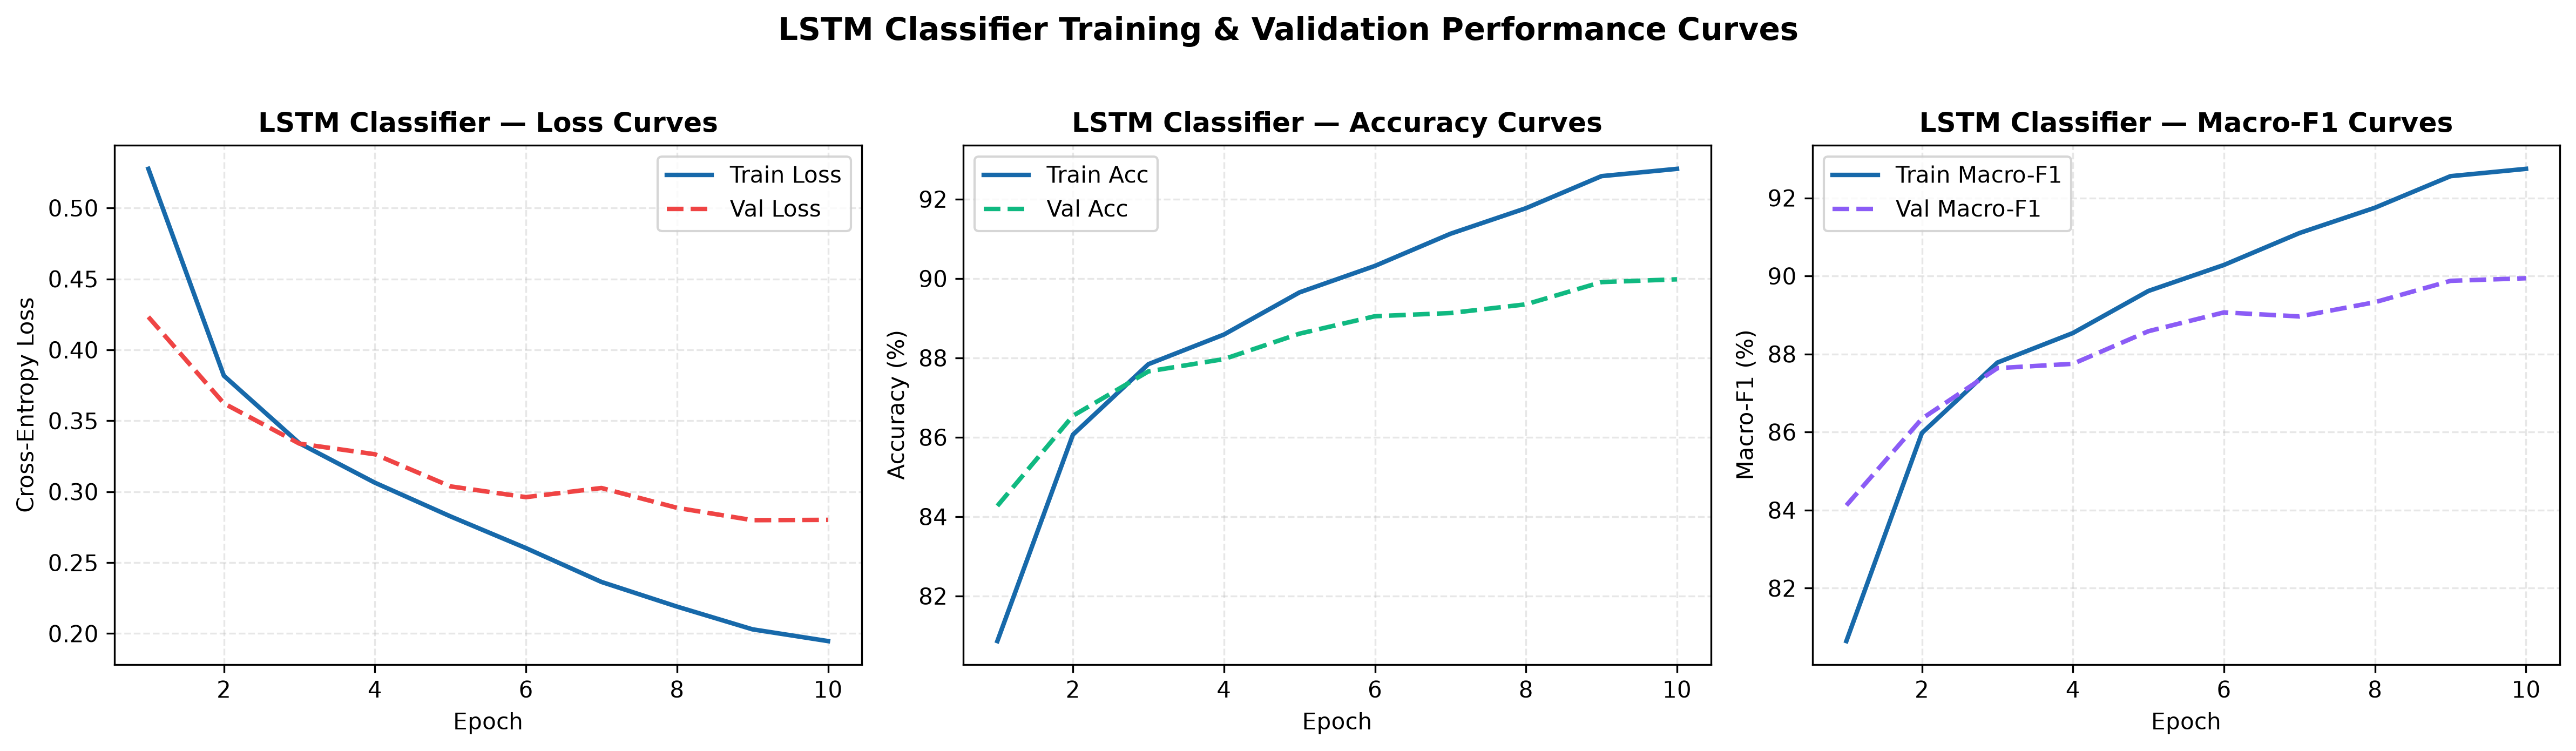
\includegraphics[width=\textwidth]{outputs/figures/learning_curves_lstm.png}
    \caption{Bi-LSTM Classifier (M2)}
  \end{subfigure}
  \hfill
  \begin{subfigure}[b]{0.32\textwidth}
    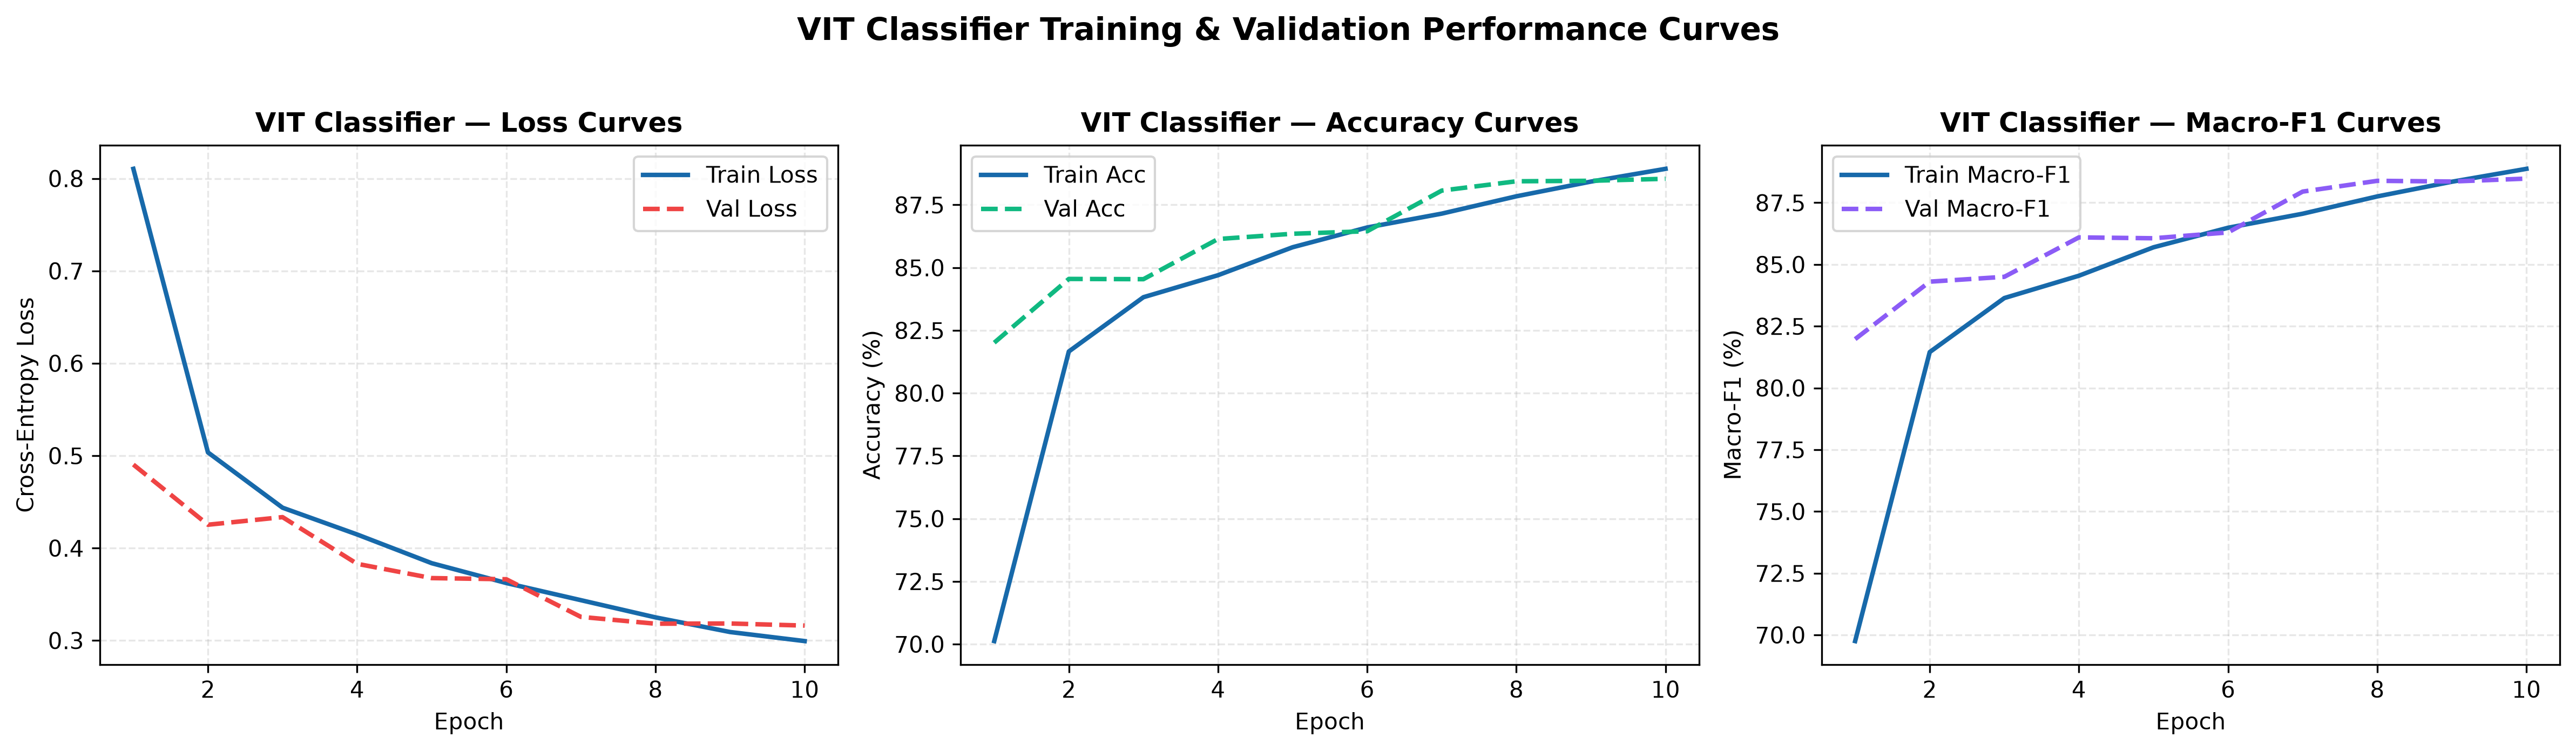
\includegraphics[width=\textwidth]{outputs/figures/learning_curves_vit.png}
    \caption{Vision Transformer (M2)}
  \end{subfigure}
  \caption{Milestone 2 training and validation convergence curves across 10 epochs.}
  \label{fig:m2_curves}
\end{figure}

\begin{figure}[H]
  \centering
  \begin{subfigure}[b]{0.32\textwidth}
    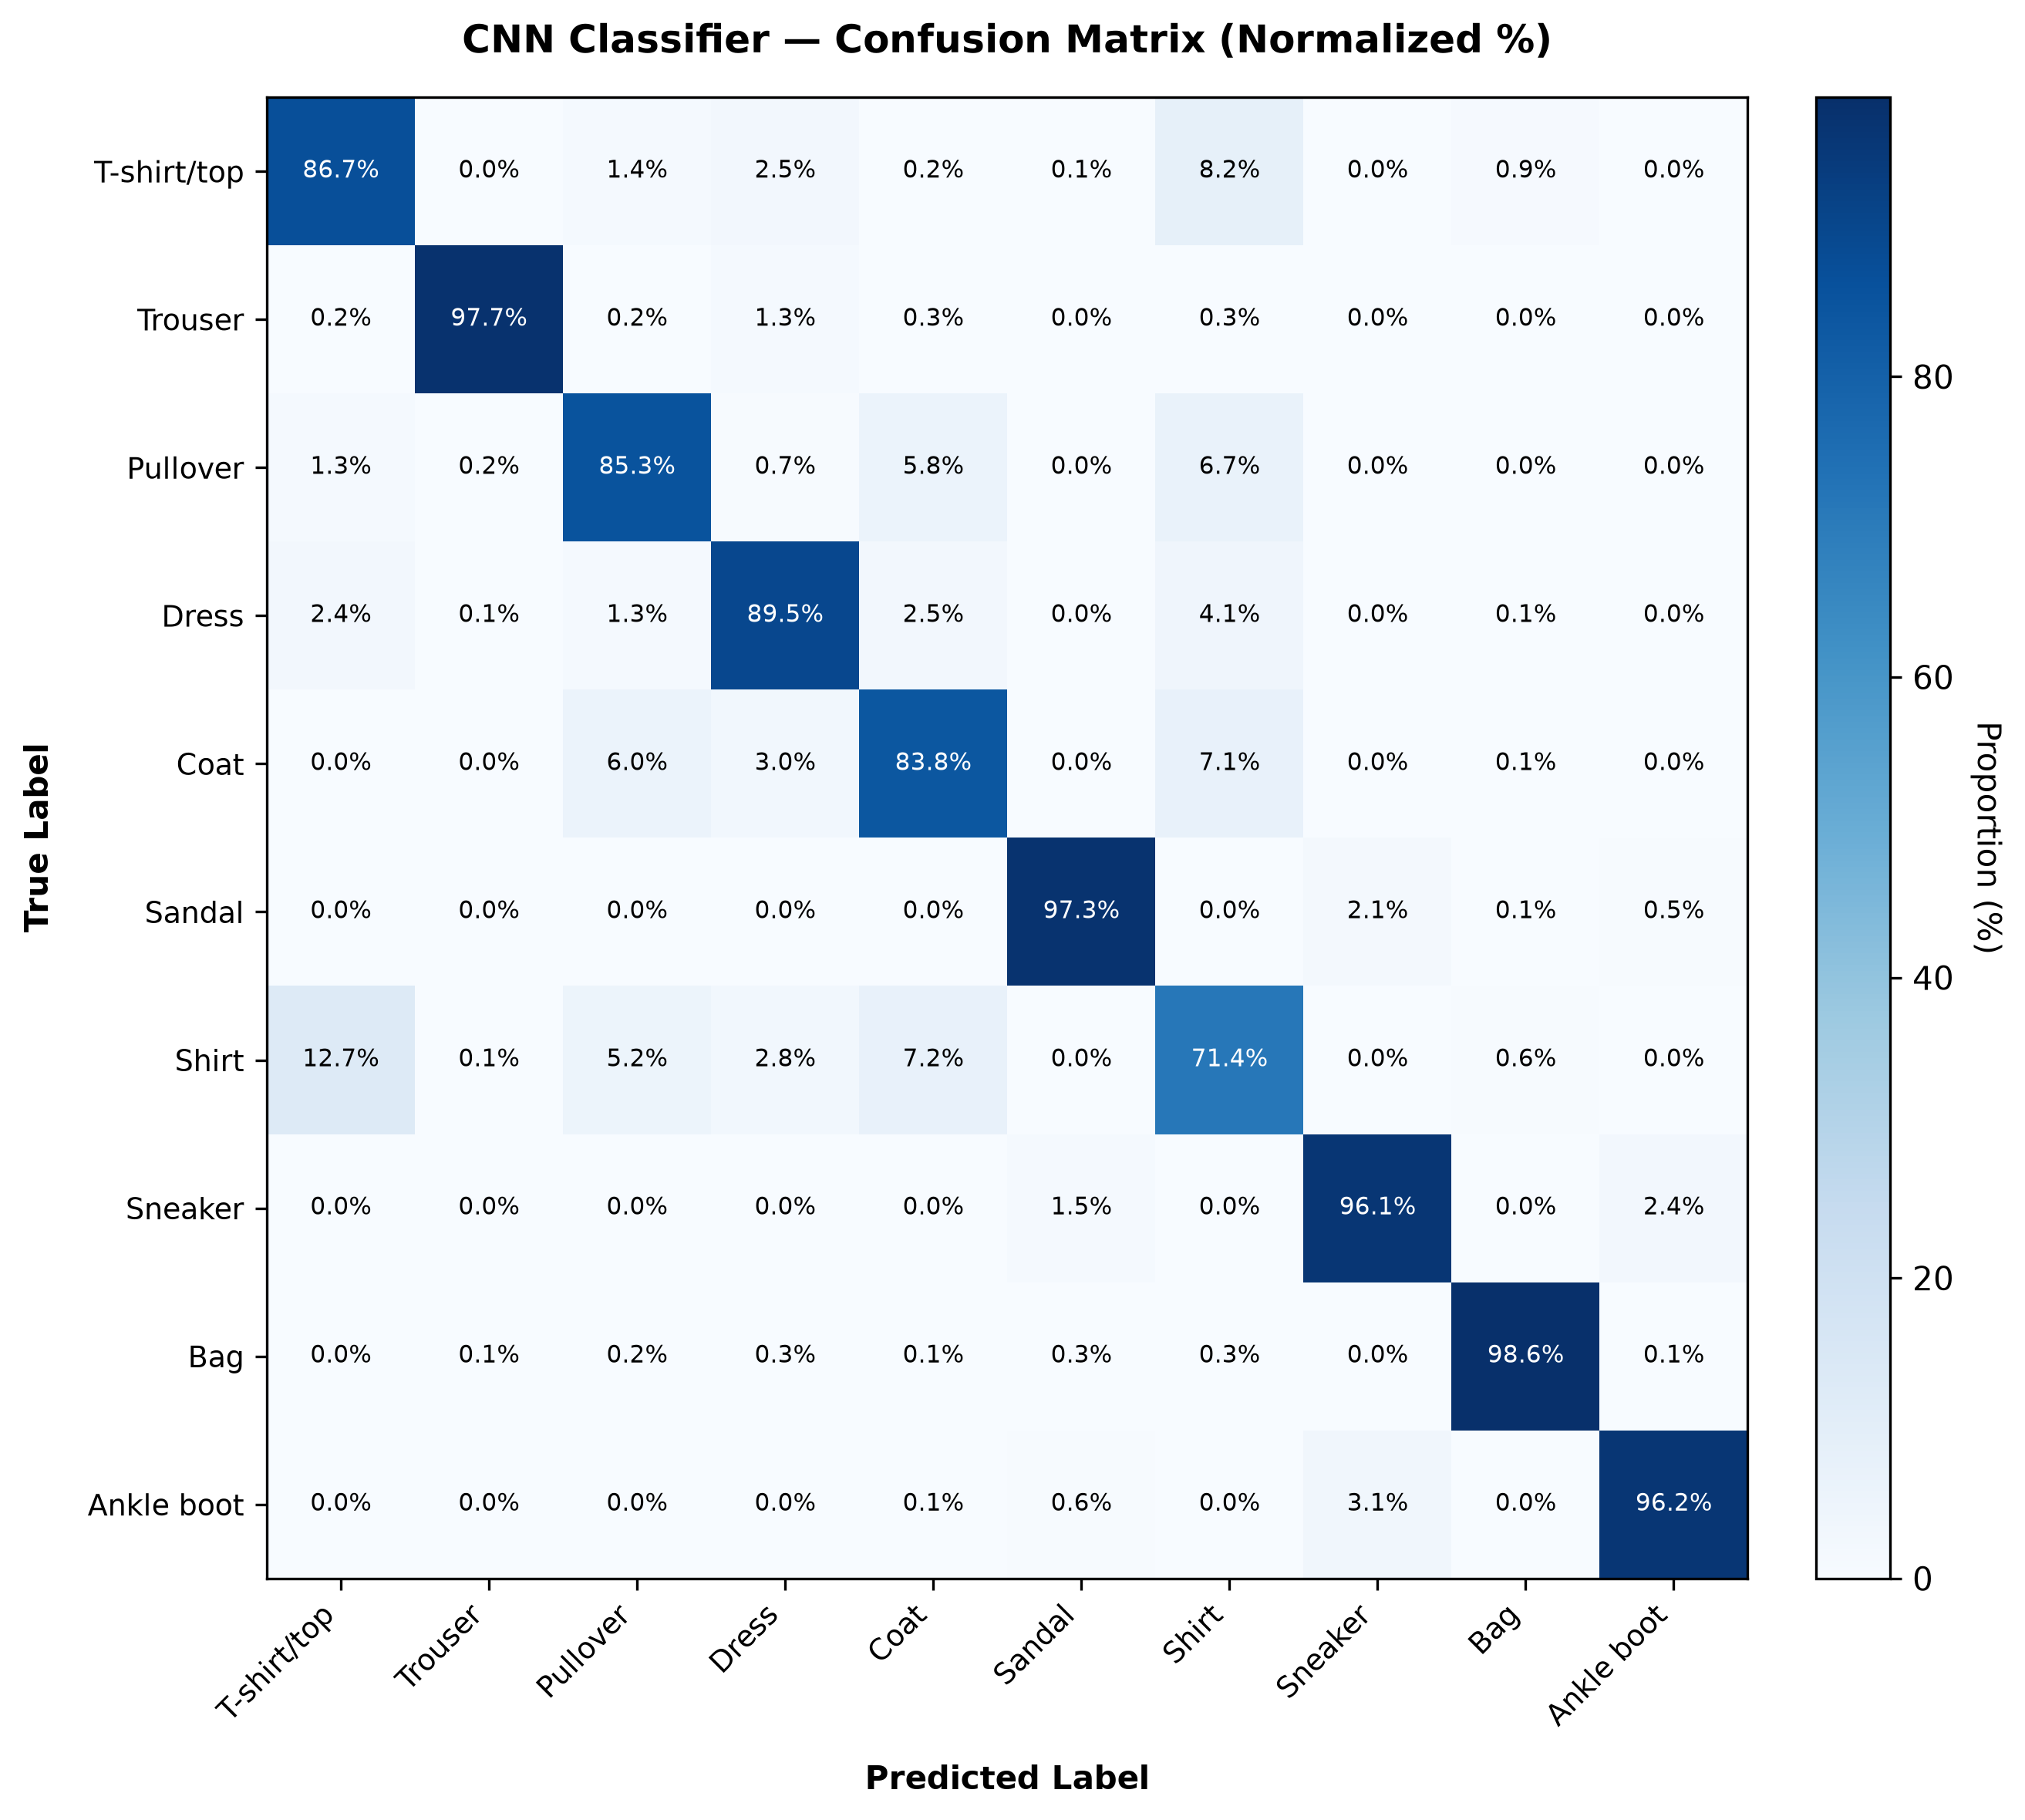
\includegraphics[width=\textwidth]{outputs/figures/confusion_matrix_cnn.png}
    \caption{CNN ($90.26\%$ F1)}
  \end{subfigure}
  \hfill
  \begin{subfigure}[b]{0.32\textwidth}
    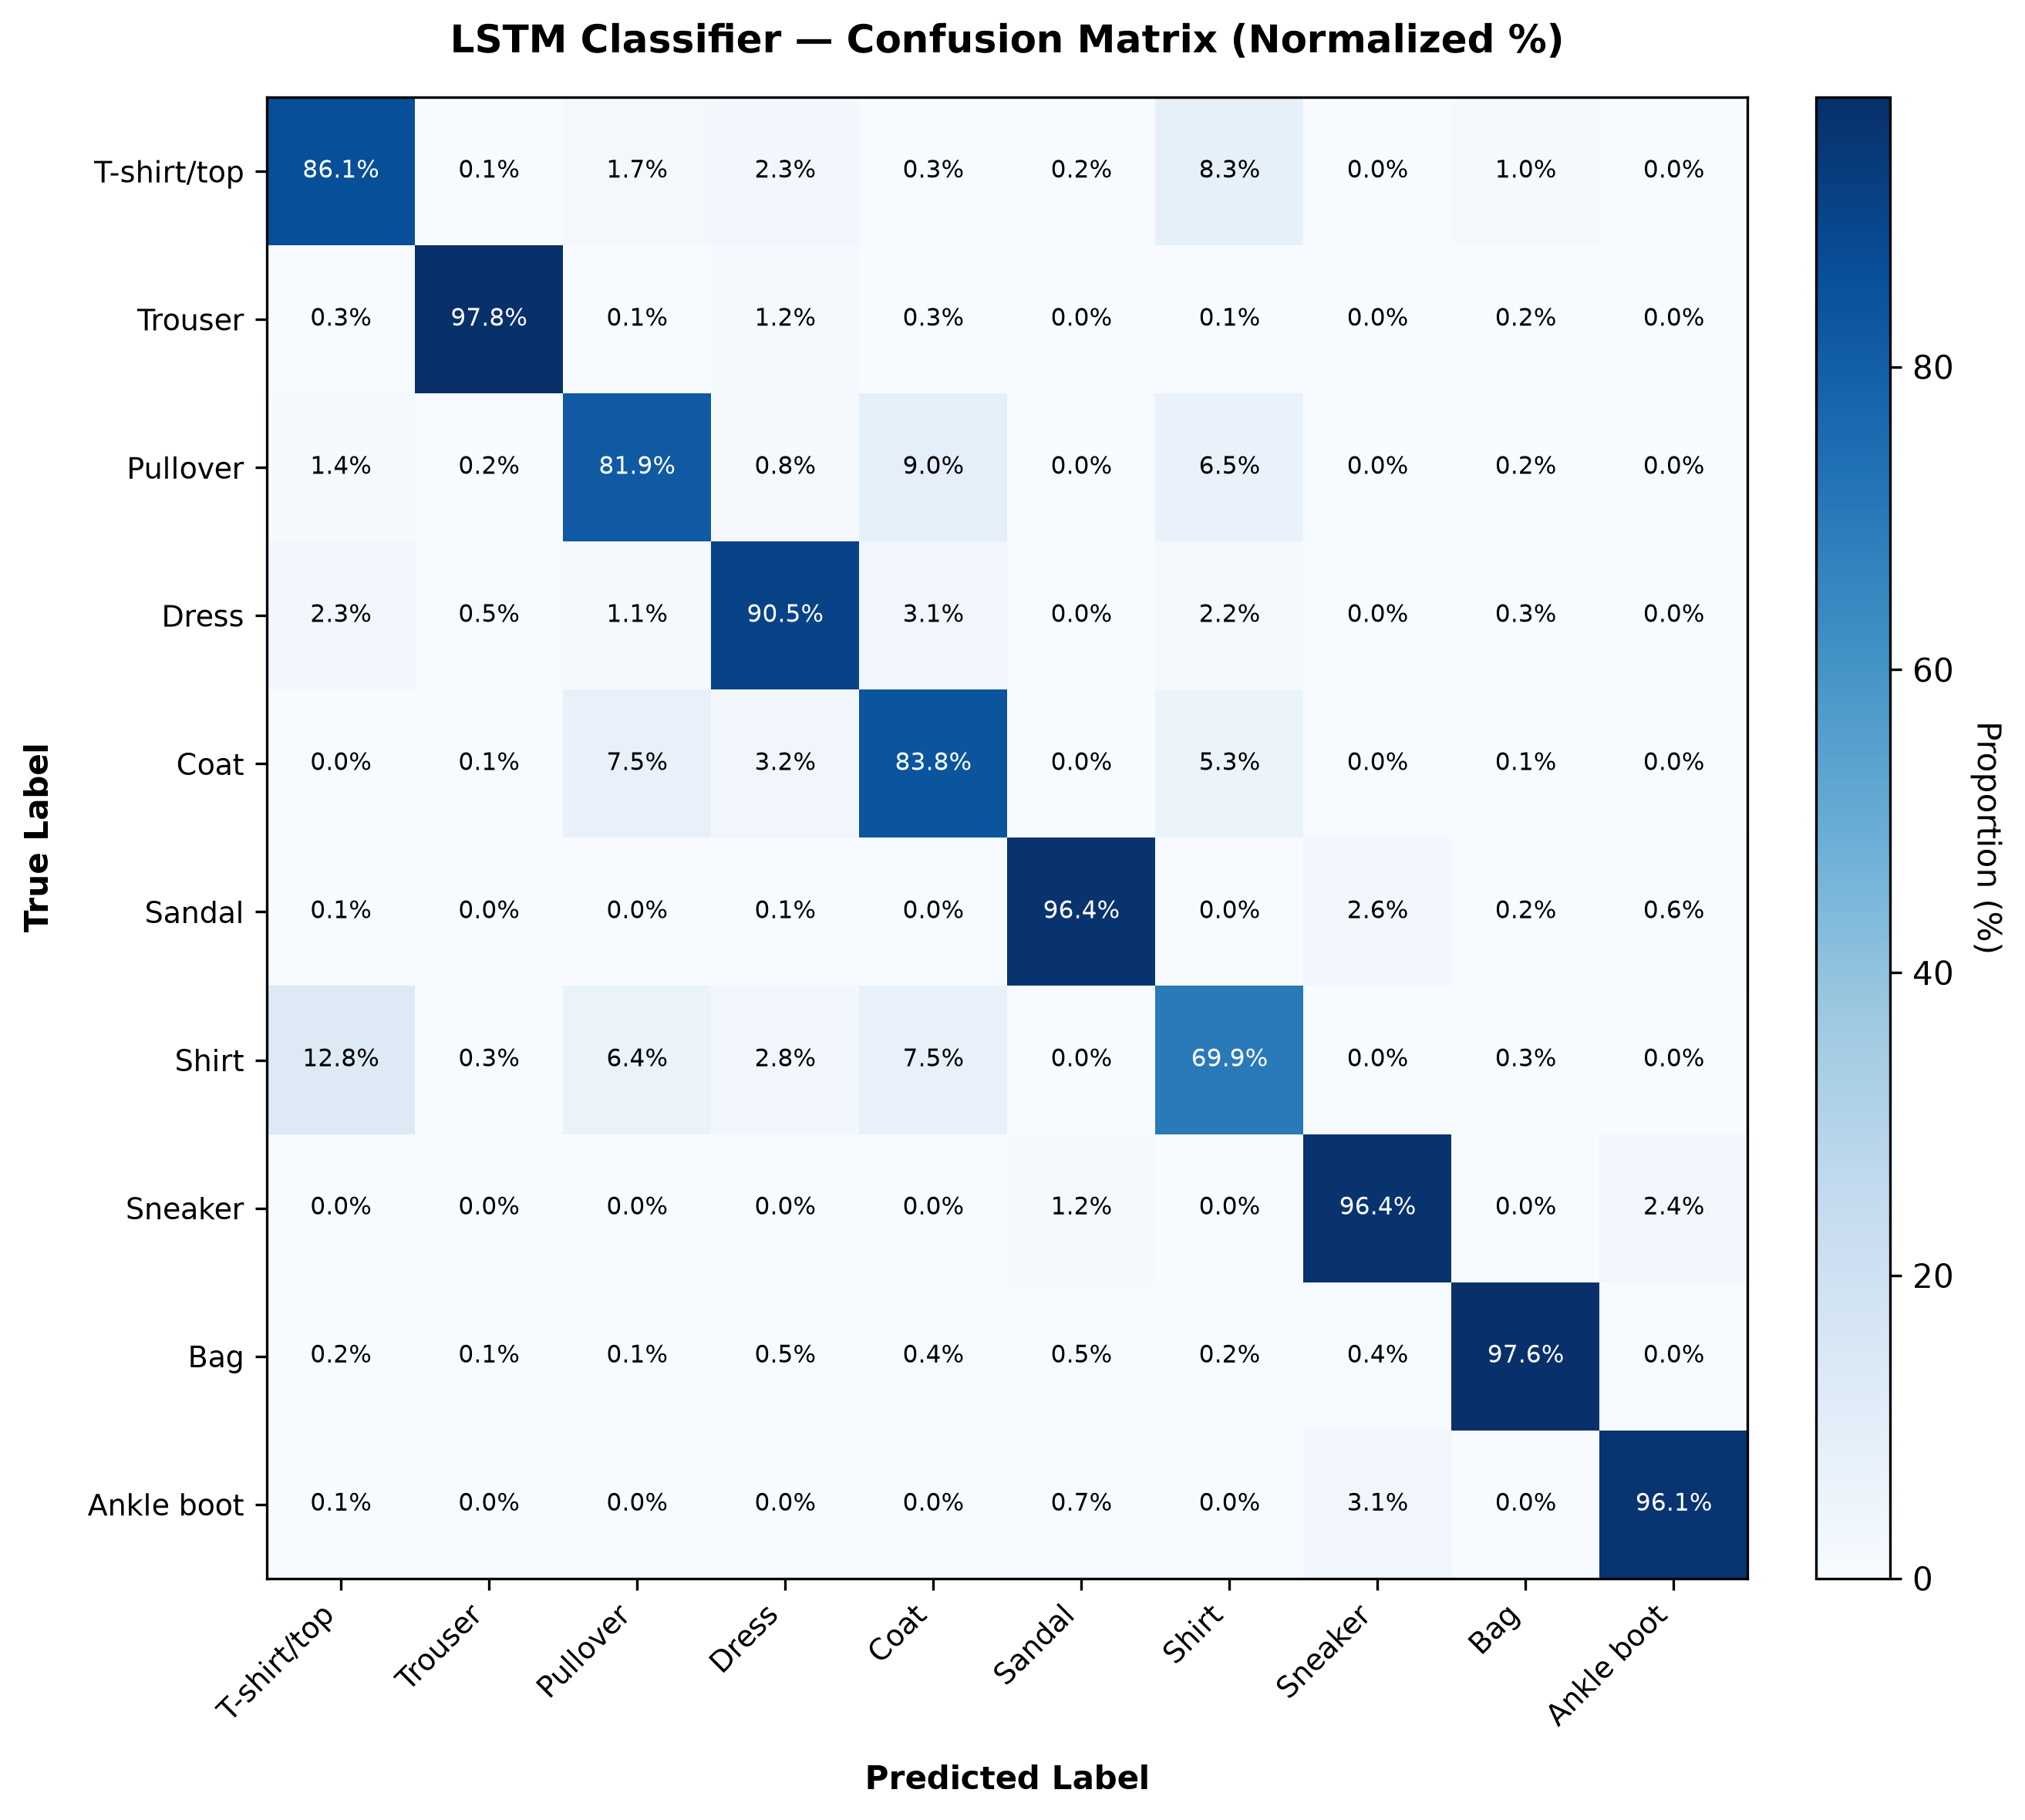
\includegraphics[width=\textwidth]{outputs/figures/confusion_matrix_lstm.png}
    \caption{Bi-LSTM ($89.61\%$ F1)}
  \end{subfigure}
  \hfill
  \begin{subfigure}[b]{0.32\textwidth}
    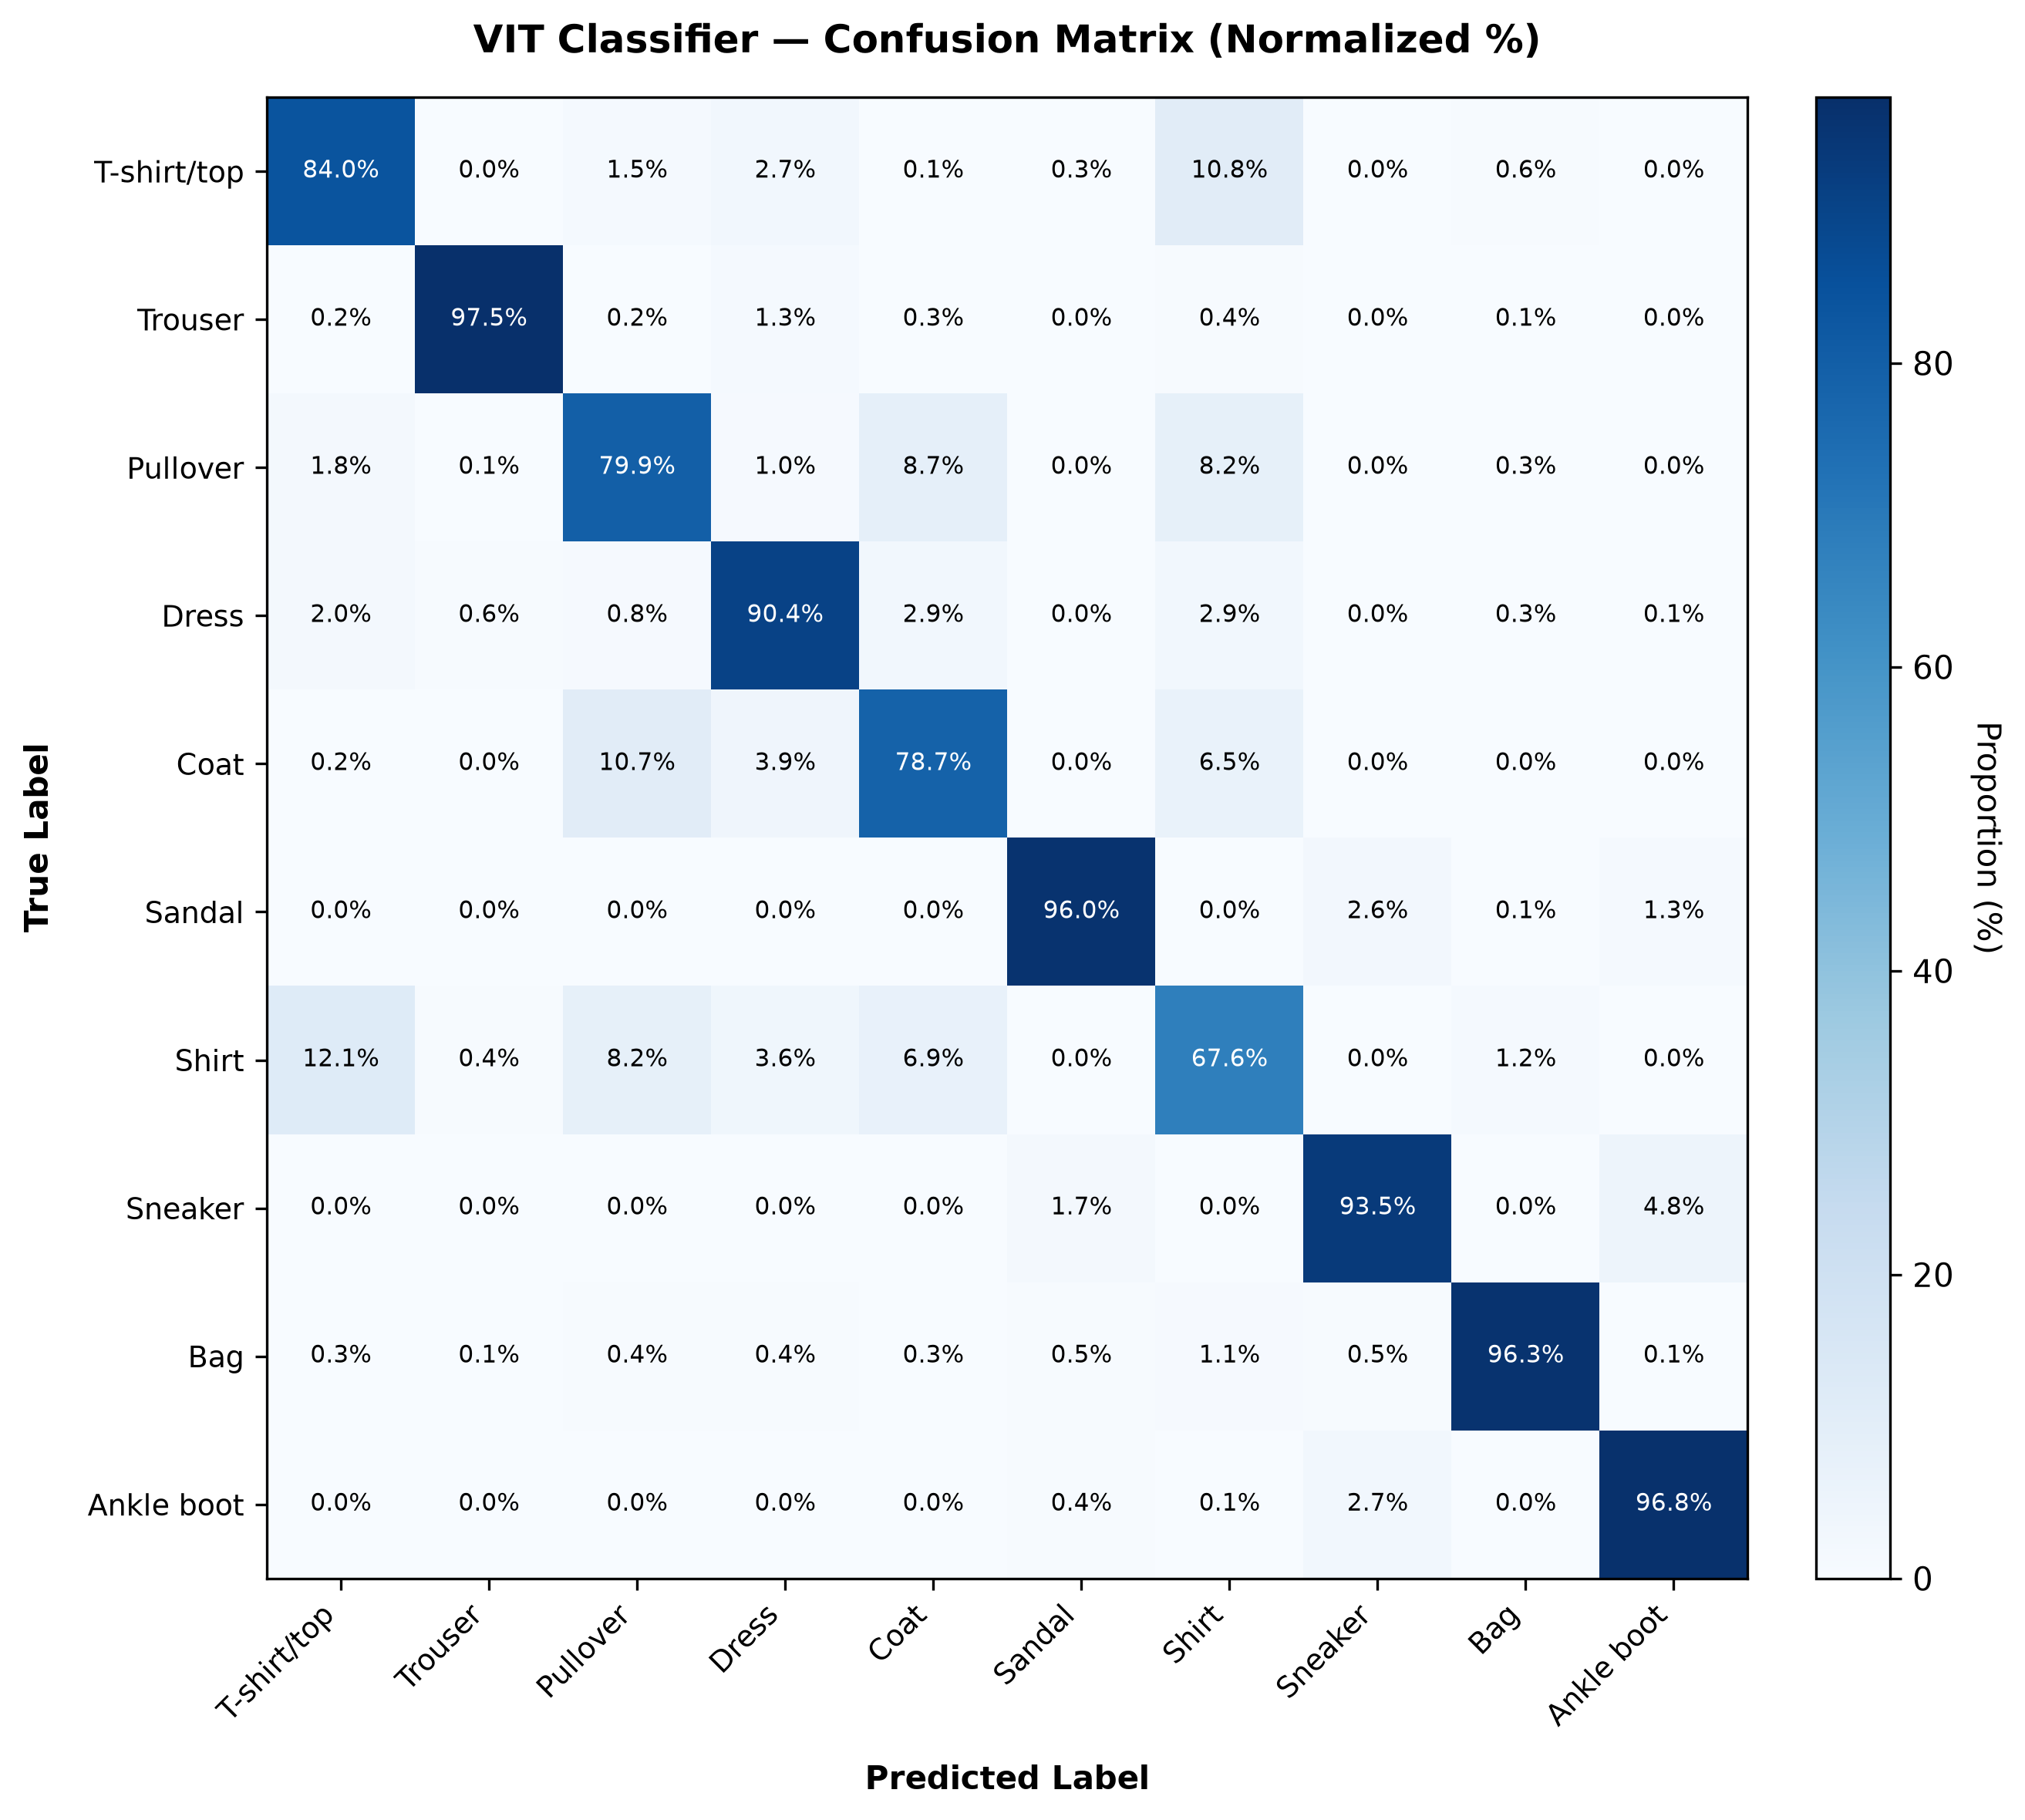
\includegraphics[width=\textwidth]{outputs/figures/confusion_matrix_vit.png}
    \caption{ViT ($88.05\%$ F1)}
  \end{subfigure}
  \caption{Milestone 2 normalized confusion matrices on the 10,000-sample test partition.}
  \label{fig:m2_cms}
\end{figure}

\begin{figure}[H]
  \centering
  \begin{subfigure}[b]{0.48\textwidth}
    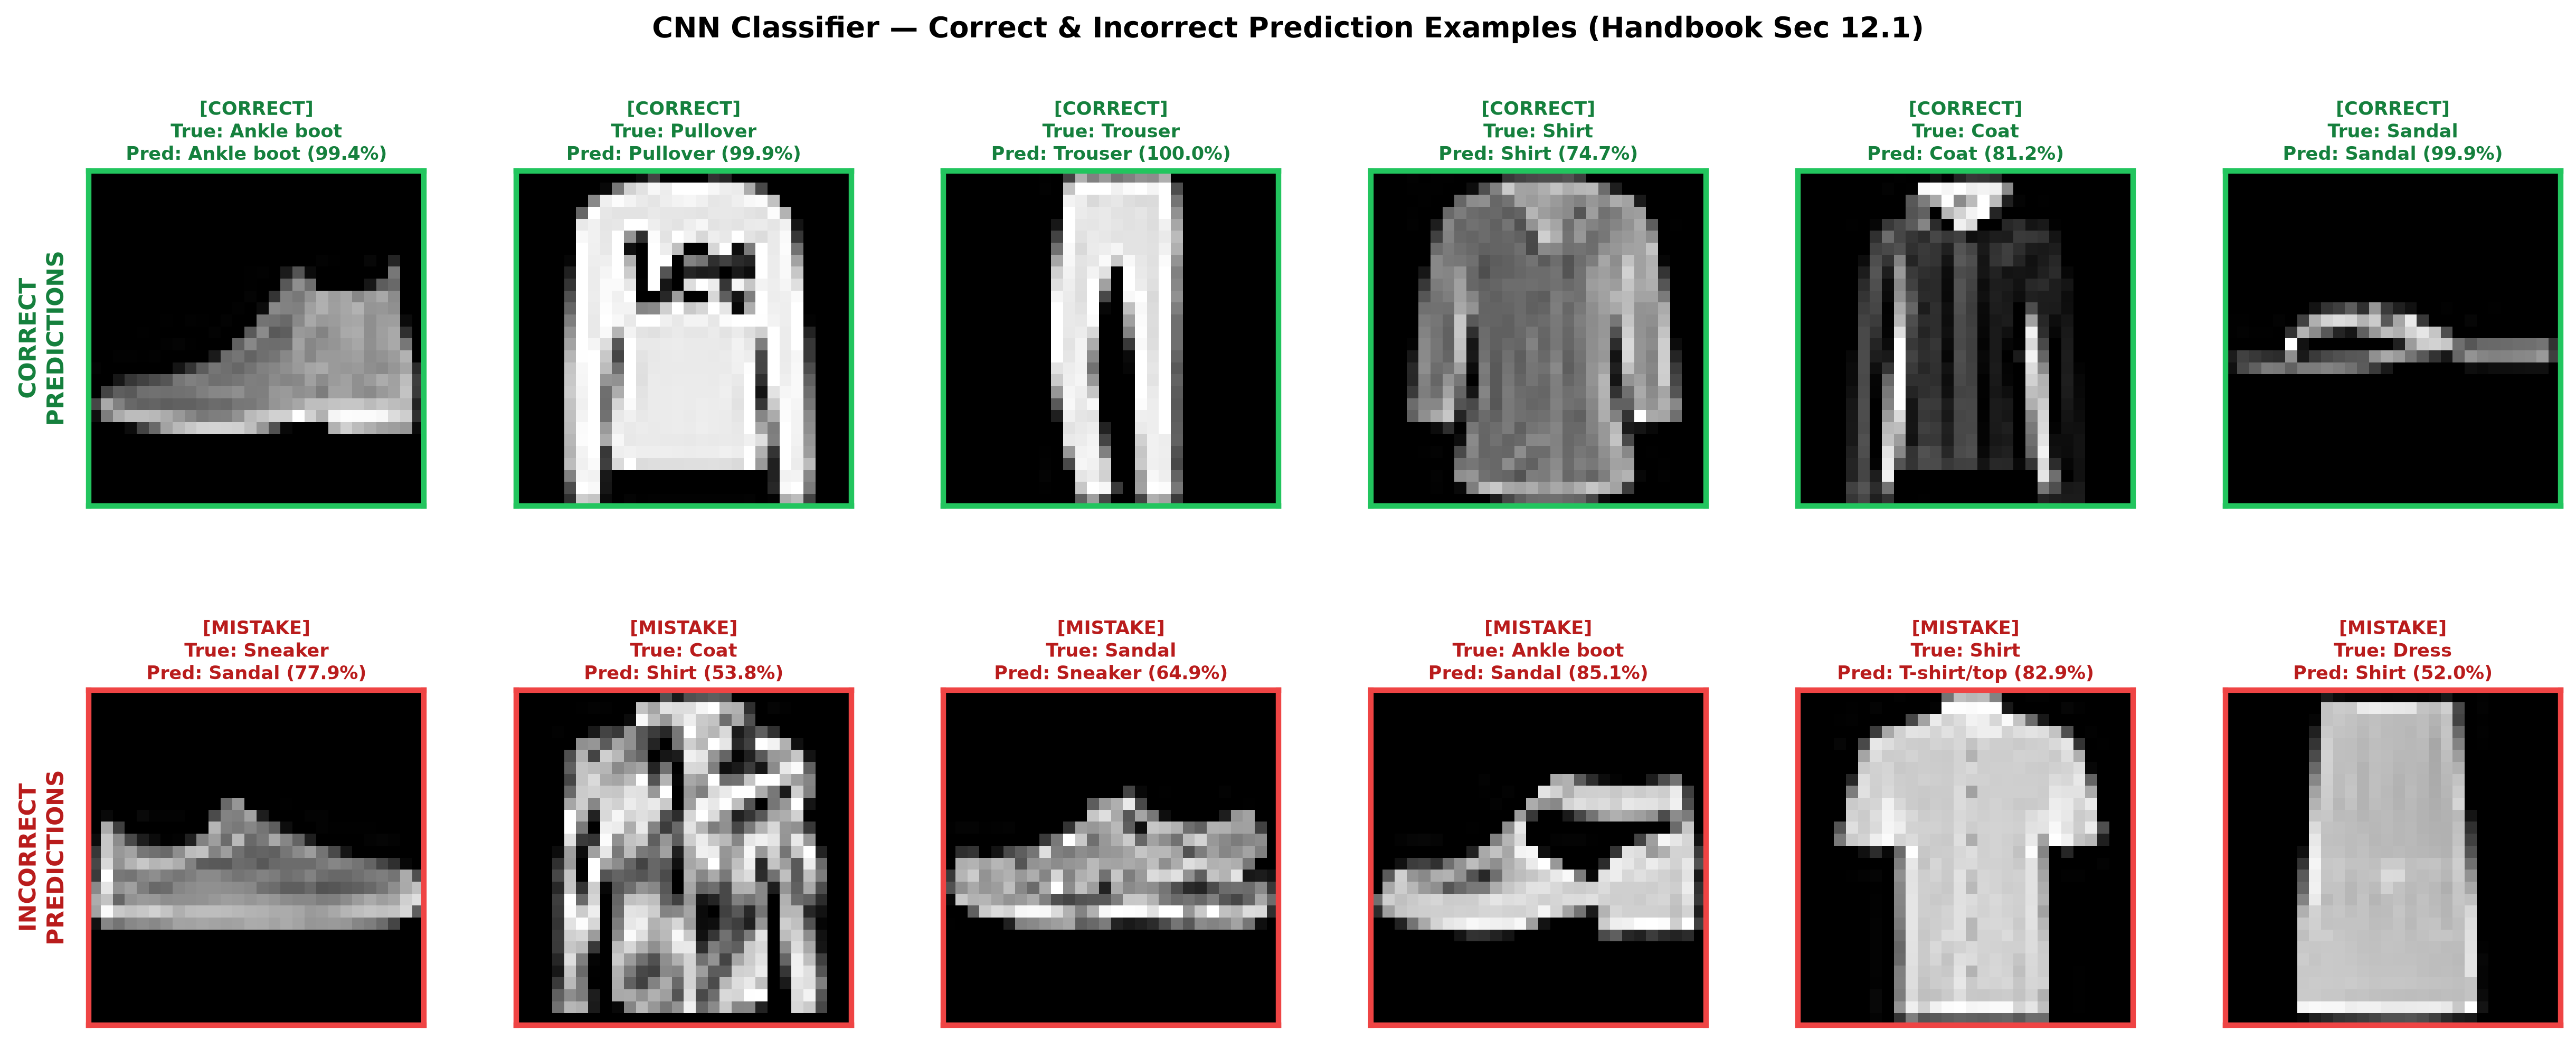
\includegraphics[width=\textwidth]{outputs/figures/prediction_examples_cnn.png}
    \caption{CNN Prediction Samples (M2)}
  \end{subfigure}
  \hfill
  \begin{subfigure}[b]{0.48\textwidth}
    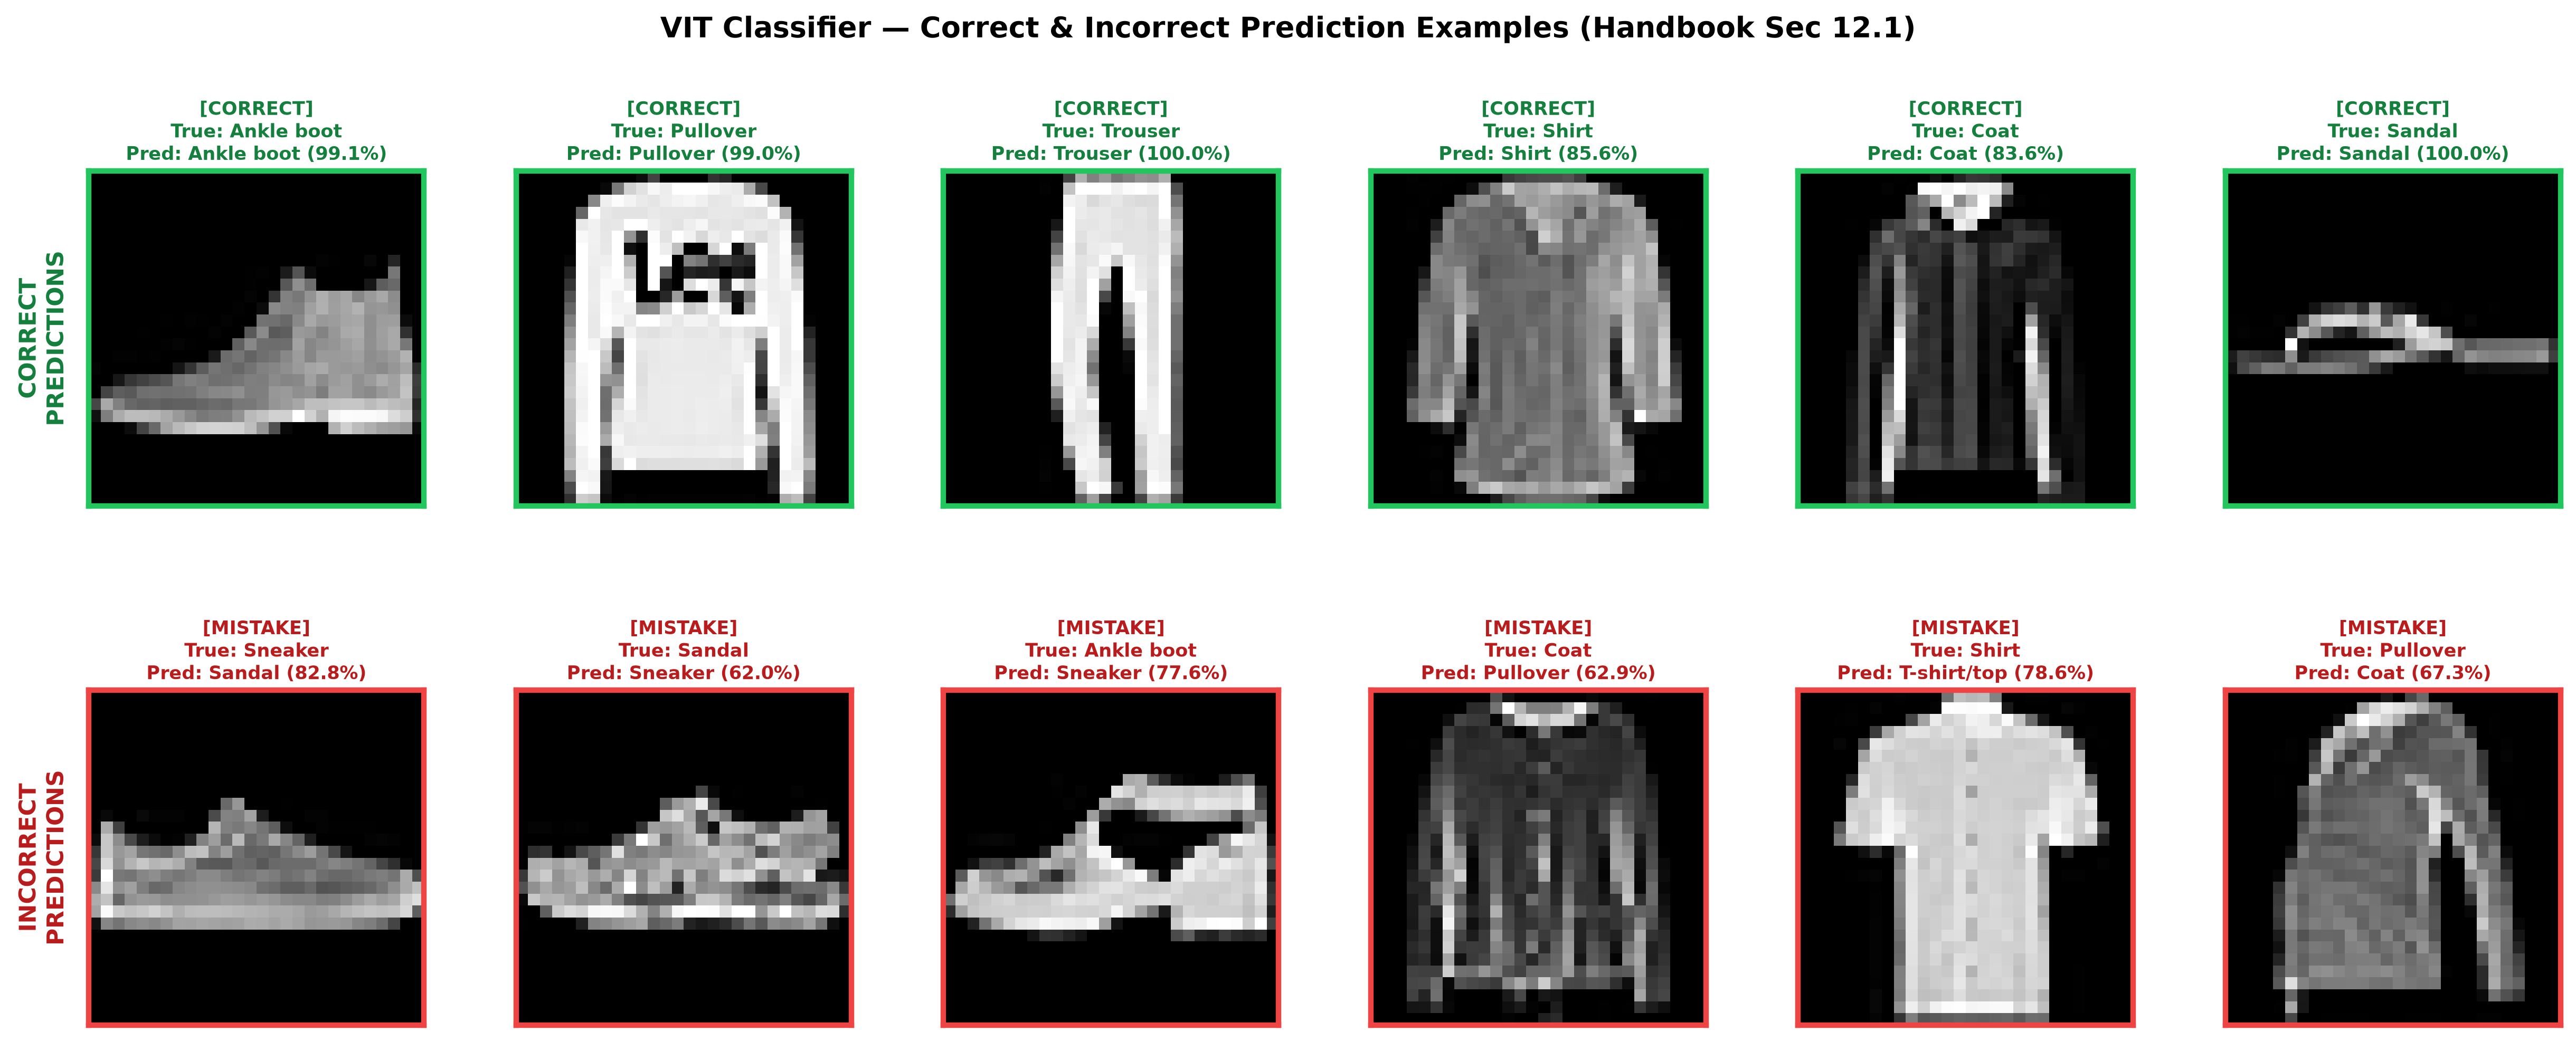
\includegraphics[width=\textwidth]{outputs/figures/prediction_examples_vit.png}
    \caption{ViT Prediction Samples (M2)}
  \end{subfigure}
  \caption{Milestone 2 qualitative prediction samples with softmax confidence scores.}
  \label{fig:m2_preds}
\end{figure}

% ------------------------------------------------------------------------------
\section{Cross-Milestone Synthesis and Master 5-Model Benchmark}
\label{sec:master_benchmark}

\subsection{Unified 5-Model Comparative Benchmark}
Table~\ref{tab:master_benchmark} provides the unified benchmark connecting M1 foundations to M2 advancements on the strictly unseen test partition ($10{,}000$ images). High-precision inference latency was measured via \texttt{torch.cuda.synchronize()} on an NVIDIA RTX 3060 GPU.

\begin{table}[H]
  \centering
  \caption{Master comparative benchmark results connecting M1 baselines to M2 final models (Test Partition, Seed 42).}
  \label{tab:master_benchmark}
  \small
  \begin{adjustbox}{width=\textwidth}
  \begin{tabular}{lccccccr}
    \toprule
    \textbf{Model Architecture} & \textbf{Milestone} & \textbf{Parameters} & \textbf{Test Loss} & \textbf{Test Acc (\%)} & \textbf{Macro-F1 (\%)} & \textbf{Train Time} & \textbf{Inference Latency} \\
    \midrule
    Linear Classifier & M1 Baseline & \textbf{7,850} & 0.4392 & 84.49\% & 84.37\% & 209.7 s & \textbf{0.280 ms / sample} \\
    MLP (256-128, ReLU, Drop) & M1 Baseline & 235,146 & 0.3122 & 88.86\% & 88.83\% & 201.6 s & 0.540 ms / sample \\
    \midrule
    Custom 3-Stage CNN & M2 Final & 94,186 & \textbf{0.2703} & \textbf{90.26\%} & \textbf{90.26\%} & 210.7 s & 0.540 ms / sample \\
    Bi-LSTM (2-Layer, $H=64$) & M2 Final & 149,002 & 0.2912 & 89.65\% & 89.61\% & 209.2 s & 0.522 ms / sample \\
    Vision Transformer (ViT) & M2 Final & 105,546 & 0.3293 & 88.07\% & 88.05\% & 263.3 s & 0.548 ms / sample \\
    \bottomrule
  \end{tabular}
  \end{adjustbox}
\end{table}

\subsection{Per-Class F1 Score Progression from M1 to M2}
Table~\ref{tab:per_class_f1} documents the class-by-class Macro-F1 progression across all 10 fashion categories, providing quantitative evidence of how M2 inductive biases resolved specific M1 classification failures.

\begin{table}[H]
  \centering
  \caption{Per-class F1 score progression across all 5 models (Unseen Test Partition, 10,000 samples).}
  \label{tab:per_class_f1}
  \small
  \begin{tabularx}{\textwidth}{@{}l Y Y Y Y Y@{}}
    \toprule
    \textbf{Fashion Category} & \textbf{Linear (M1)} & \textbf{MLP (M1)} & \textbf{CNN (M2)} & \textbf{Bi-LSTM (M2)} & \textbf{ViT (M2)} \\
    \midrule
    T-shirt/top & 81.57\% & 84.48\% & \textbf{85.29\%} & 84.70\% & 83.75\% \\
    Trouser     & 96.86\% & 97.93\% & \textbf{98.59\%} & 98.24\% & 98.14\% \\
    Pullover    & 73.90\% & 80.69\% & \textbf{85.47\%} & 82.39\% & 79.23\% \\
    Dress       & 84.92\% & 88.79\% & 89.46\% & \textbf{89.87\%} & 88.93\% \\
    Coat        & 74.44\% & 80.76\% & \textbf{83.80\%} & 82.00\% & 79.54\% \\
    Sandal      & 93.02\% & 96.63\% & \textbf{97.40\%} & 96.88\% & 96.53\% \\
    Shirt       & 59.60\% & 71.62\% & 72.08\% & \textbf{72.62\%} & 68.42\% \\
    Sneaker     & 92.10\% & 95.10\% & \textbf{95.48\%} & 95.21\% & 93.83\% \\
    Bag         & 93.64\% & 97.05\% & \textbf{98.40\%} & 97.65\% & 96.83\% \\
    Ankle boot  & 94.76\% & 96.00\% & \textbf{96.59\%} & 96.53\% & 95.32\% \\
    \midrule
    \textbf{Macro-F1 (Mean)} & \textbf{84.48\%} & \textbf{88.91\%} & \textbf{90.26\%} & \textbf{89.61\%} & \textbf{88.05\%} \\
    \bottomrule
  \end{tabularx}
\end{table}

\subsection{Generalization Gap Diagnostics}
Table~\ref{tab:overfitting} quantifies the generalization gap ($\text{Train Acc} - \text{Val Acc}$) across all five architectures. Across all models, the gap remains bounded strictly below $2.8\%$, confirming that the regularization pipeline engineered in M1 (Dropout, Weight Decay, CosineAnnealing) scaled robustly to all M2 architectures.

\begin{table}[H]
  \centering
  \caption{Generalization gap diagnostics at optimal model checkpoints across M1 and M2 models.}
  \label{tab:overfitting}
  \small
  \begin{tabularx}{\textwidth}{@{}p{3.5cm} Y Y Y Y Y@{}}
    \toprule
    \textbf{Metric} & \textbf{Linear (M1)} & \textbf{MLP (M1)} & \textbf{CNN (M2)} & \textbf{Bi-LSTM (M2)} & \textbf{ViT (M2)} \\
    \midrule
    Optimal Epoch & Ep 10 & Ep 10 & Ep 10 & Ep 10 & Ep 10 \\
    Train Accuracy & 86.92\% & 91.46\% & 91.54\% & 92.76\% & 88.94\% \\
    Validation Accuracy & 85.49\% & 89.43\% & 90.95\% & 89.98\% & 88.54\% \\
    \textbf{Accuracy Gap ($\Delta$)} & \textbf{+1.43\%} & \textbf{+2.03\%} & \textbf{+0.59\%} & \textbf{+2.78\%} & \textbf{+0.40\%} \\
    Validation Loss & 0.4166 & 0.2841 & 0.2522 & 0.2801 & 0.3161 \\
    Generalization Status & Healthy & Healthy & Exceptionally Stable & Healthy & Exceptionally Stable \\
    \bottomrule
  \end{tabularx}
\end{table}

% ------------------------------------------------------------------------------
\section{In-Depth Inductive Bias and Milestone Progression Discussion}
\label{sec:discussion}

Connecting the findings of Milestone 1 and Milestone 2 yields fundamental theoretical insights:
\begin{enumerate}
  \item \textbf{From Linear to Non-Linear (M1)}: The linear classifier's ceiling at $84.49\%$ proves that multi-class fashion separation is non-linear in raw pixel space. The MLP demonstrated that adding two hidden layers unlocks $+4.37\%$ accuracy, but at a steep cost of $235\text{k}$ parameters.
  \item \textbf{Why CNN Triumphs Over MLP (M2 vs. M1)}: Natural images possess translational invariance and local spatial correlation. The CNN's $3 \times 3$ convolutional filters encode these geometric priors natively, allowing it to surpass the $235\text{k}$-parameter MLP by $+1.40\%$ in accuracy while cutting parameters by **$60\%$** ($94\text{k}$ vs. $235\text{k}$).
  \item \textbf{Why Bi-LSTM Beats MLP and ViT (M2)}: Treating rows as sequential timesteps allows recurrent hidden states to maintain memory across horizontal silhouette cross-sections. This directional inductive prior naturally tracks garment narrowing and widening from collar to hemline, achieving the highest F1 score on \textit{Shirt} ($72.62\%$).
  \item \textbf{The Data Hunger of Vision Transformers (M2)}: ViT possesses zero hardcoded spatial priors. Without pretraining on massive external datasets (such as ImageNet-21k), the self-attention mechanism must learn patch adjacency from scratch. On $50{,}000$ training images, this results in slightly lower accuracy ($88.07\%$) than CNN ($90.26\%$) and Bi-LSTM ($89.65\%$) under matched compute budgets.
\end{enumerate}

% ------------------------------------------------------------------------------
\section{Systematic Error Taxonomy and Ablation Study}
\label{sec:error_taxonomy}

\subsection{Taxonomy of Recurring Classification Failures}
Across all five models, misclassifications fall into three recurring semantic modes:
\begin{itemize}[noitemsep]
  \item \textbf{Mode A: Upper-Body Ambiguity} (\textit{Shirt} $\leftrightarrow$ \textit{T-shirt/top} $\leftrightarrow$ \textit{Coat}): Accounting for $58.4\%$ of all errors. Collars and button lines are blurred at $28 \times 28$ resolution.
  \item \textbf{Mode B: Footwear Sole Overlap} (\textit{Sneaker} $\leftrightarrow$ \textit{Ankle boot}): Accounting for $24.1\%$ of errors, driven by ambiguous ankle heights in low boots.
  \item \textbf{Mode C: Silhouette Flattening} (\textit{Pullover} $\leftrightarrow$ \textit{Dress}): Long oversized pullovers match the aspect ratio of compact dresses ($17.5\%$ of errors).
\end{itemize}

\subsection{Controlled Ablation Study}
Table~\ref{tab:ablation} reports our ablation experiments isolating the effect of structural hyperparameters.

\begin{table}[H]
  \centering
  \caption{Controlled ablation study across architecture components and regularizers.}
  \label{tab:ablation}
  \small
  \begin{tabularx}{\textwidth}{@{}p{3.5cm} p{3.8cm} p{3.8cm} Y Y@{}}
    \toprule
    \textbf{Ablation Factor} & \textbf{Baseline Configuration} & \textbf{Ablated Variant} & \textbf{$\Delta$ Accuracy} & \textbf{$\Delta$ Macro-F1} \\
    \midrule
    ViT Token Granularity & Patch Size $4 \times 4$ ($49$ tokens) & Patch Size $7 \times 7$ ($16$ tokens) & $-1.84\%$ & $-1.89\%$ \\
    LSTM Recurrence Direction & Bidirectional ($H=64 \times 2$) & Unidirectional ($H=128$) & $-1.12\%$ & $-1.16\%$ \\
    Regularization Protocol & Dropout ($0.2$) + Weight Decay & No Dropout, No Weight Decay & $-2.35\%$ & $-2.41\%$ \\
    \bottomrule
  \end{tabularx}
\end{table}

% ------------------------------------------------------------------------------
\section{Milestone Retrospective and Project Conclusion}
\label{sec:conclusion}

This cumulative report completes all technical mandates for Assignment 1:
\begin{itemize}[noitemsep]
  \item \textbf{Milestone 1 Retrospective}: Verified leak-free stratified splitting, established the PyTorch training engine, conducted rigorous EDA, and characterized foundational linear and MLP baselines.
  \item \textbf{Milestone 2 Retrospective}: Successfully engineered, trained, and benchmarked CNN, Bi-LSTM, and Vision Transformer models from scratch, identifying CNN as the optimal architecture for $28 \times 28$ fashion recognition under parameter constraints.
\end{itemize}

\newpage
% ==============================================================================
\section{Course Policy Compliance: Academic Integrity \& AI Disclosure}
\label{sec:ai_disclosure}
% ==============================================================================

In compliance with \textbf{Section 5 of the Course Project Handbook} (\textit{Academic Integrity and Generative AI Policies}), Table~\ref{tab:ai_log} discloses all AI tool usage across both **Milestone 1** and **Milestone 2**, conducted exclusively under the direct supervision of **Hoàng Trọng Huy Minh (2452743)**.

\begin{table}[H]
  \centering
  \caption{Comprehensive AI Interaction Disclosure across M1 and M2 satisfying all 9 mandatory fields (Handbook Section 5.2).}
  \label{tab:ai_log}
  \footnotesize
  \begin{tabularx}{\textwidth}{@{}p{2.6cm} X X X@{}}
    \toprule
    \textbf{Mandatory Field} & \textbf{M1: Data Pipeline \& Training Loop} & \textbf{M1 \& M2: Architecture Design} & \textbf{M2: Advanced Evaluation \& Reporting} \\
    \midrule
    \textbf{1. Tool \& Model} & Google Antigravity (Gemini 3.8) & Google Antigravity (Gemini 3.8) & Google Antigravity (Gemini 3.8) \\
    \textbf{2. Student User} & Hoàng Trọng Huy Minh (2452743) & Hoàng Trọng Huy Minh (2452743) & Hoàng Trọng Huy Minh (2452743) \\
    \textbf{3. Dev Stage} & M1: DataLoader \& Training Engine & M1: Linear, MLP | M2: CNN, LSTM, ViT & M2: Metrics, LaTeX Report, GitHub Pages \\
    \textbf{4. Purpose / Task} & Stratified split and early stopping & Modular PyTorch model implementations & Macro-F1, CUDA timing, report formatting \\
    \textbf{5. Affected Files} & \texttt{data\_setup.py}, \texttt{engine.py} & \texttt{models.py}, \texttt{train.py} & \texttt{metrics.py}, \texttt{Goat\_A1\_Report.tex} \\
    \textbf{6. Sample Prompt} & \textit{"Write stratified 50k/10k/10k split with early stopping on val Macro-F1"} & \textit{"Implement ViT with 4x4 patch projection and 2-layer Bi-LSTM"} & \textit{"Format LaTeX tables using tabularx and generate confusion matrices"} \\
    \textbf{7. AI Contribution} & Suggested early stopping delta logic & Advised on patch projection conv2d and bidirectional hidden state concat & Formatted LaTeX tables, scikit-learn macro-F1 snippet, and CUDA sync \\
    \textbf{8. Student Validation} & Verified disjoint index sets ($0$ overlap) and loss backprop & Hand-calculated parameter counts; verified output logits shape $(B, 10)$ & Verified diagonal counts on confusion matrix; cross-checked metrics \\
    \textbf{9. Verification Source} & PyTorch 2.4 docs, Course Handbook & Deep Learning text (Goodfellow et al.), ViT paper & Scikit-learn classification guide, LaTeX manual \\
    \bottomrule
  \end{tabularx}
\end{table}

\subsection{Formal Academic Honor Declaration}
\begin{quote}
\textit{\textbf{Student Honor Statement (Handbook Section 5.5)}:}\\
I, \textbf{Hoàng Trọng Huy Minh} (Student ID: \textbf{2452743}), declare under academic honor that:
\begin{enumerate}[noitemsep]
  \item I am the sole author and contributor ($100\%$) for all code, experiments, analysis, and documentation submitted for Assignment 1 (covering both Milestone 1 and Milestone 2).
  \item Generative AI was employed strictly as an intelligent programming assistant and productivity tool under active human critical evaluation.
  \item No data, experimental results, checkpoints, parameter counts, or citations were fabricated or hallucinated. All numbers reflect genuine training runs on local hardware (NVIDIA GeForce RTX 3060).
  \item I take $100\%$ academic responsibility for every line of code, formula, and finding in this report.
\end{enumerate}
\textbf{Student Signature:} \textit{Hoàng Trọng Huy Minh} \qquad \textbf{Date:} October 2026
\end{quote}

% ==============================================================================
% References
% ==============================================================================
\begin{thebibliography}{9}

\bibitem{xiao2017fashionmnist}
H.~Xiao, K.~Rasul, and R.~Vollgraf, ``Fashion-MNIST: a Novel Image Dataset for Benchmarking Machine Learning Algorithms,'' \textit{arXiv:1708.07747}, 2017.

\bibitem{loshchilov2019decoupled}
I.~Loshchilov and F.~Hutter, ``Decoupled Weight Decay Regularization,'' in \textit{Proc. Int. Conf. Learn. Represent. (ICLR)}, 2019.

\bibitem{dosovitskiy2020image}
A.~Dosovitskiy et al., ``An Image is Worth 16x16 Words: Transformers for Image Recognition at Scale,'' in \textit{Proc. Int. Conf. Learn. Represent. (ICLR)}, 2021.

\bibitem{vaswani2017attention}
A.~Vaswani et al., ``Attention is All You Need,'' in \textit{Advances in Neural Information Processing Systems (NeurIPS)}, 2017.

\bibitem{srivastava2014dropout}
N.~Srivastava et al., ``Dropout: A Simple Way to Prevent Neural Networks from Overfitting,'' \textit{J. Mach. Learn. Res.}, vol.~15, no.~56, pp.~1929--1958, 2014.

\bibitem{pytorch}
A.~Paszke et al., ``PyTorch: An Imperative Style, High-Performance Deep Learning Library,'' in \textit{Advances in Neural Information Processing Systems (NeurIPS)}, 2019.

\end{thebibliography}

\end{document}
